\documentclass[c]{beamer}

\usepackage[utf8]{inputenc}
\usepackage[francais]{babel}
\usepackage{adjustbox}

% figures
\setbeamerfont{caption}{size=\tiny}

% margins
\setbeamersize{text margin left=3em, text margin right=3em}

% puces
\setbeamertemplate{itemize item}[ball] % Pour le premier niveau
\setbeamertemplate{itemize subitem}[triangle] % Pour le deuxième niveau
\setbeamertemplate{itemize subsubitem}[circle] % Pour le troisième niveau

\setbeamerfont{section in toc}{size=\scriptsize}
\setbeamerfont{subsection in toc}{size=\tiny}

% links
\definecolor{links}{HTML}{2A1B81}
\hypersetup{colorlinks,linkcolor=,urlcolor=links}

% theme
\usetheme{Warsaw}


\title[High-Res satellite images for human density prediction]{High-Res Landsat-8 satellite images \\for human density prediction}

\author{Youcef Kacer}

\institute{\href{http://www.github.com/ykacer/}{www.github.com/ykacer}}

\date{2017,January 25\textsuperscript{th}}

%color
\colorlet{rouge}{red} % rename colors in frencj
\colorlet{grisfonce}{darkgray}
\colorlet{titre}{yellow}
\definecolor{vertmoyen}{RGB}{51,110,23} % custom rgb color
\definecolor{rouge}{HTML}{DD0000} % custom html color

\begin{document}
\begin{frame}
\titlepage
\logo{\includegraphics[height=5mm]{images/logo/TelecomParisTech_logo_200_01.png}}
\end{frame}

\begin{frame}
\tableofcontents
\end{frame}

\section{Presentation}
\begin{frame}
\tableofcontents[currentsection]
\end{frame}

\begin{frame}
\begin{itemize}
\item Population census is expensive using conventional methods\\
  \begin{itemize}
  \item 180 millions euros in France (\href{http://www.assemblee-nationale.fr/13/rap-info/i1246.asp}{officials,1999})\\ 
  \end{itemize}
\item How High-resolution satellites images could explain human density?\\
\item How to transform HR satellite images to explain human density?\\
\end{itemize}
\end{frame}

\section{Landsat-8 imagery}

\subsection{Earth Covering}
\begin{frame}[label=Covering]
\tableofcontents[currentsubsection]
\end{frame}

\begin{frame}

\begin{itemize}
\item Total earth covering defined by (path,row) grid pattern and achieved every 16 days
\end{itemize}
\begin{columns}
\begin{column}{\textwidth}
\begin{overlayarea}{\linewidth}{4cm}
  \centering\vfill
  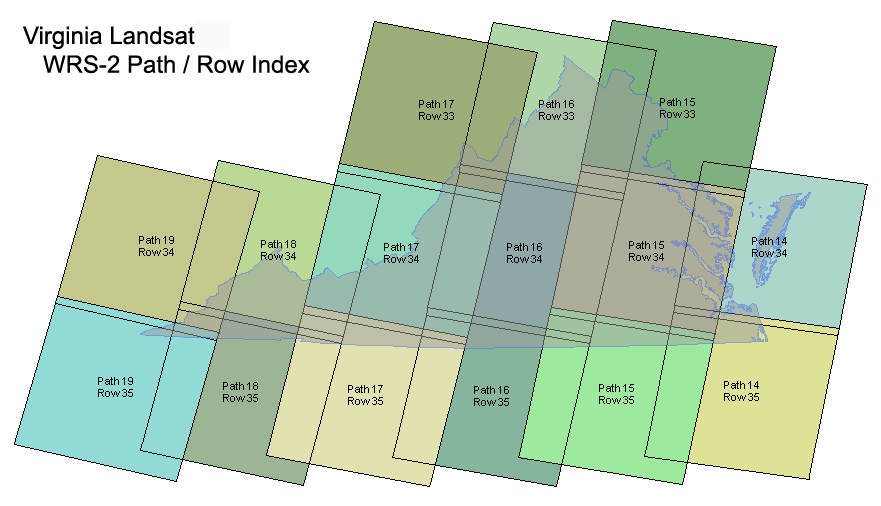
\includegraphics[scale=0.2]{images/covering/wrs.png}
\end{overlayarea}
\begin{overlayarea}{\linewidth}{1cm}
  \centering
  \tiny Landsat-8 grid covering (path,row) for Virginia ($USA$)\par
\end{overlayarea}
\end{column}
\end{columns}

\end{frame}

\subsection{Image Georeferencement}
\begin{frame}
\tableofcontents[currentsubsection]
\end{frame}

\begin{frame}
\begin{itemize}
 \item Landsat-8 images are georeferenced which means each pixel has (x,y) meter coordinates in a certain Projection Coordinates 
System (\begin{itshape}ex: UTM, Lambert IV, Lambert 93, Web Mercator,...\end{itshape})
\end{itemize}

\begin{columns}
\begin{column}{0.30\textwidth}
\begin{overlayarea}{\linewidth}{5cm}
  \centering\vfill
  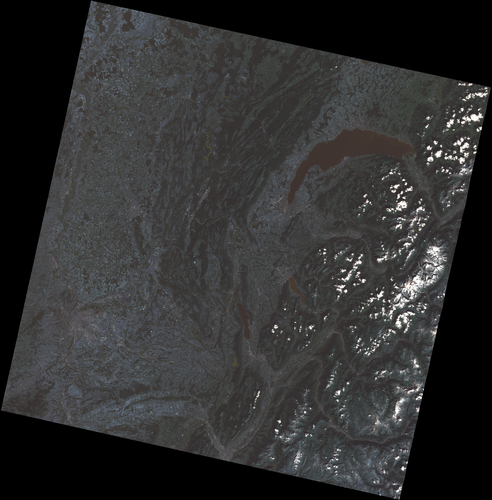
\includegraphics[scale=0.2]{images/georeferencing/Thonon_landsat.png}
\end{overlayarea}
\end{column}
\begin{column}{0.30\textwidth}
\begin{overlayarea}{\linewidth}{1cm}
  \centering
  \tiny Landsat-8 Eastern-France image path=$196$,row=$028$ georeferenced in $UTM$ system (image containing city Thonon-les-Bains)\par
\end{overlayarea}
\end{column}

\begin{column}{0.30\textwidth}
\begin{block}{\scriptsize UTM corner coordinates}
{\scriptsize
 \begin{itemize}
  \item upper-left (,)\\
  \item upper-right (,)\\
  \item bottom-right (,)\\
  \item bottom-left (,)\\
  \item center (,)\\
 \end{itemize}
}
\end{block}
\end{column}
\end{columns}

\end{frame}

\begin{frame}
\begin{itemize}
 \item Landast-8 georeferencement can be checked comparing with another georeferenced source like $IGN$ using a $SIG$ (open source $QGIS$).
\end{itemize}

\begin{columns}[t]
\begin{column}{0.30\textwidth}
%\begin{overlayarea}{\linewidth}{0.0cm}
%  \centering
%  \par
%\end{overlayarea}
\begin{overlayarea}{\linewidth}{3cm}
  \centering\vfill
  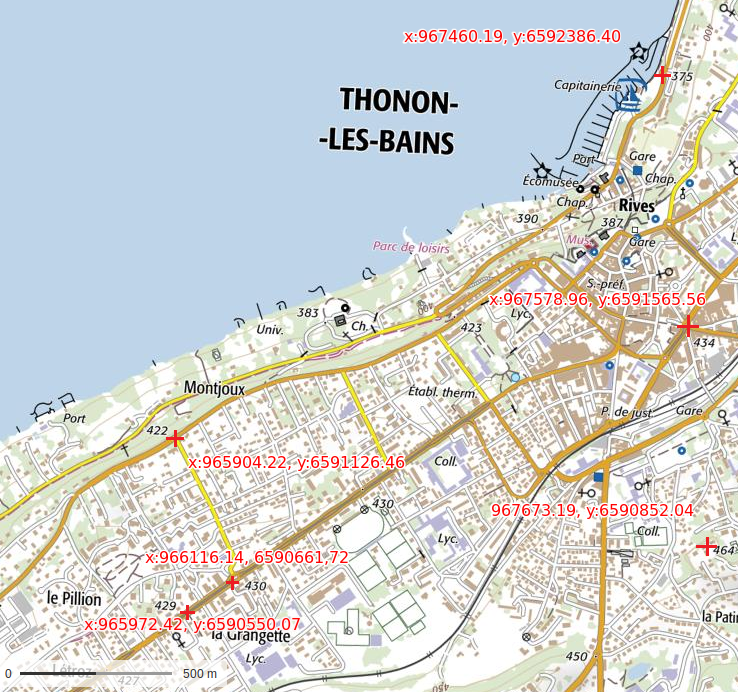
\includegraphics[height=2.5cm,width=2.5cm]{images/georeferencing/ign-points-Thonon.png}
\end{overlayarea}
\begin{overlayarea}{\linewidth}{2cm}
  \centering
  \scriptsize IGN image georeferenced in $Lambert$ $93$ system\par
\end{overlayarea}
\end{column}
\begin{column}{0.30\textwidth}
%\begin{overlayarea}{\linewidth}{0.0cm}
%  \centering
%  \par
%\end{overlayarea}
\begin{overlayarea}{\linewidth}{3cm}
  \centering\vfill
  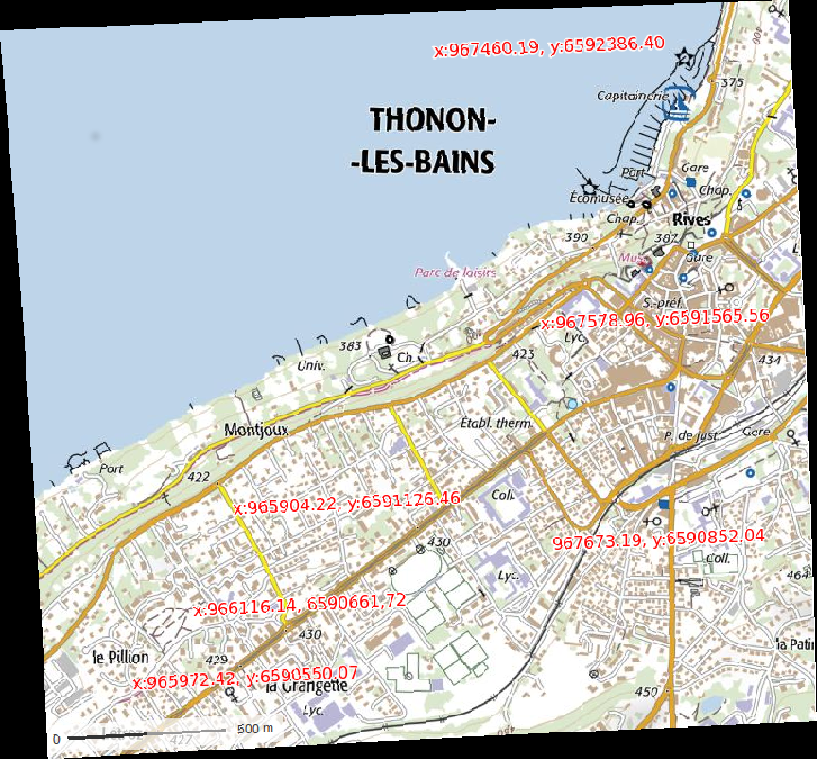
\includegraphics[height=2.5cm,width=2.5cm]{images/georeferencing/qgis-resultat.png}
\end{overlayarea}
\begin{overlayarea}{\linewidth}{2cm}
  \centering
  \scriptsize Then IGN image is tranformed to be georeferenced in $UTM$ system\par
\end{overlayarea}
\end{column}
\begin{column}{0.30\textwidth}
%\begin{overlayarea}{\linewidth}{0.0cm}
%  \centering
%  \par
%\end{overlayarea}
\begin{overlayarea}{\linewidth}{3cm}
  \centering\vfill
  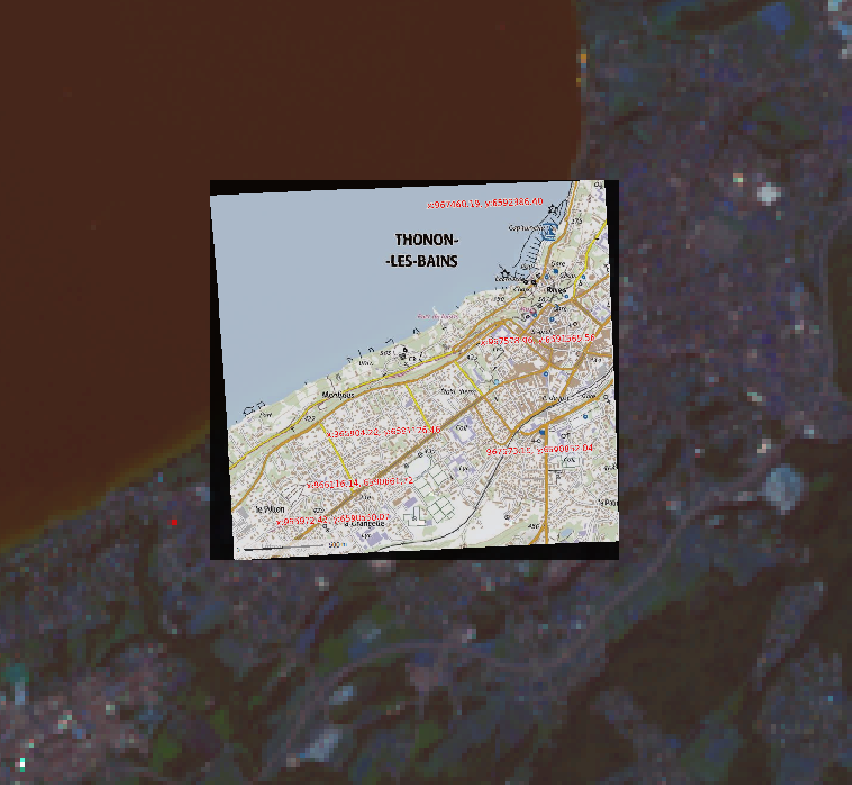
\includegraphics[height=2.5cm,width=2.5cm]{images/georeferencing/qgis-superposition0.png}
\end{overlayarea}
\begin{overlayarea}{\linewidth}{2cm}
  \centering
  \scriptsize Superposition of IGN and Landsat-8 images both georeferenced in $UTM$ system\par
\end{overlayarea}
\end{column}
\end{columns}

\end{frame}

\section{Importing Data}

\subsection{Image query}
\begin{frame}
 \begin{itemize}
 \item Query images from \href{https://earthexplorer.usgs.gov/}{\begin{itshape}U.S geological Survey\end{itshape}} website with criterias:
 \begin{itemize}
  \item cloud covering $\le$ 20\%\\
  \item day acquisition\\
  \item between May, 2013 and September, 2013\\ 
 \end{itemize}
 
\end{itemize}

\begin{columns}[t]
\begin{column}{0.50\textwidth}
\begin{overlayarea}{\linewidth}{4cm}
  \centering\vfill
  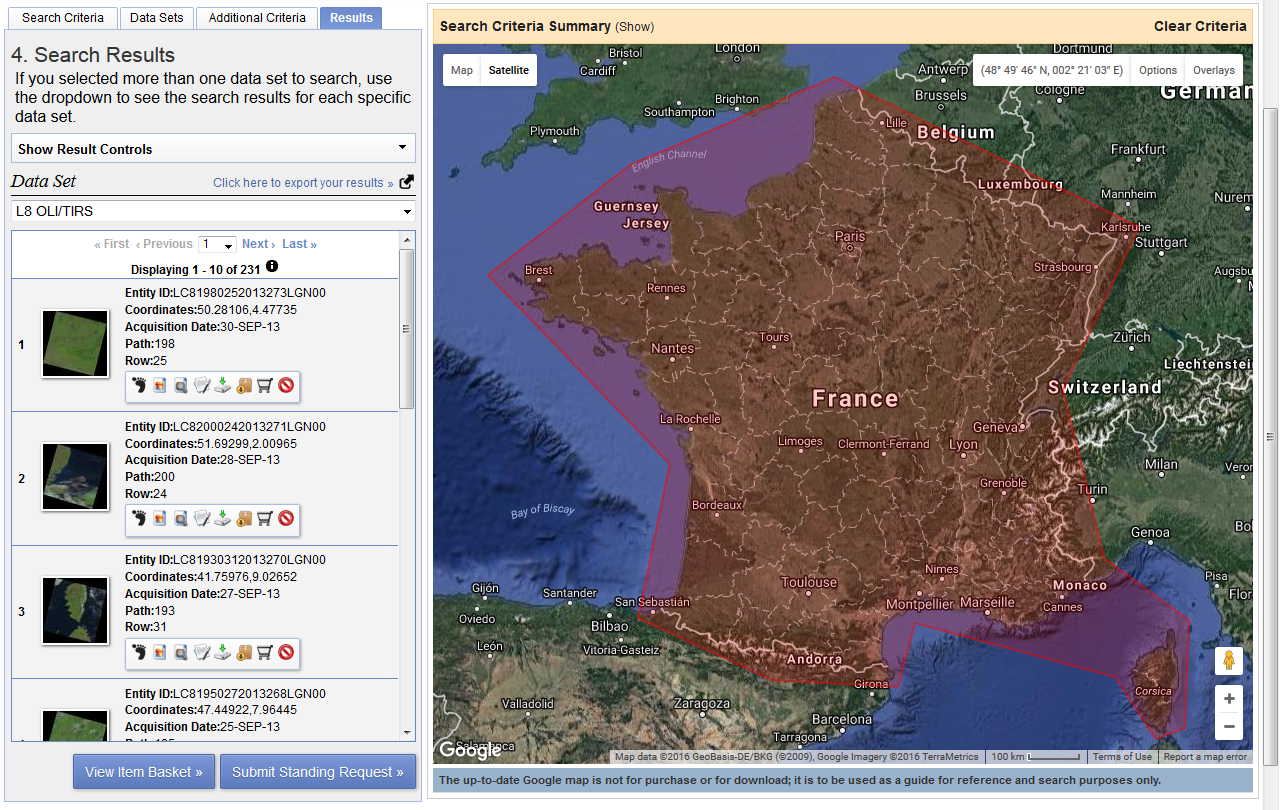
\includegraphics[scale=0.17]{images/importing/france-selection.png}
\end{overlayarea}
\begin{overlayarea}{\linewidth}{1cm}
  \centering
  \scriptsize Polygon selection on $USGS$ website\par
\end{overlayarea}
\end{column}

\begin{column}{0.50\textwidth}
\begin{overlayarea}{\linewidth}{4cm}
  \centering\vfill
  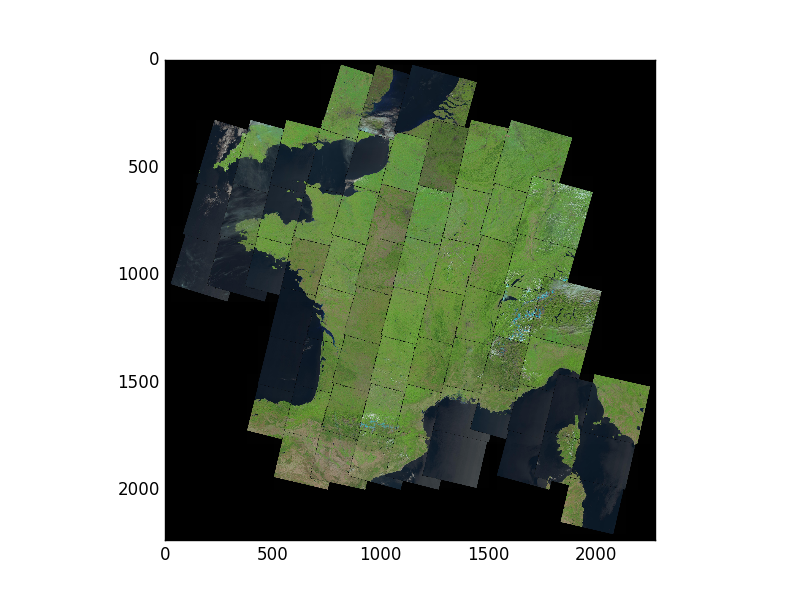
\includegraphics[scale=0.25]{images/importing/france-covering.png}
\end{overlayarea}
\begin{overlayarea}{\linewidth}{1cm}
  \centering
  \scriptsize 68 resulting datasets georeferenced in $UTM$ system\par
\end{overlayarea}
\end{column}
\end{columns}

\end{frame}

\subsection{Image bands}
\begin{frame}
 \begin{itemize}
  \item Landsat-8 dataset is composed of 
  \begin{itemize}
   \item 11 bands (OLI/TRS sensors) + 1 quality band (cloudyness of each pixel)
   \item Possible combinaison of bands to extract information (bands 4 and 5 for vegetation presence)
 \end{itemize}
\end{itemize}
 
\begin{columns}
\begin{column}{0.80\textwidth}
\begin{overlayarea}{\linewidth}{4cm}
  \centering\vfill
  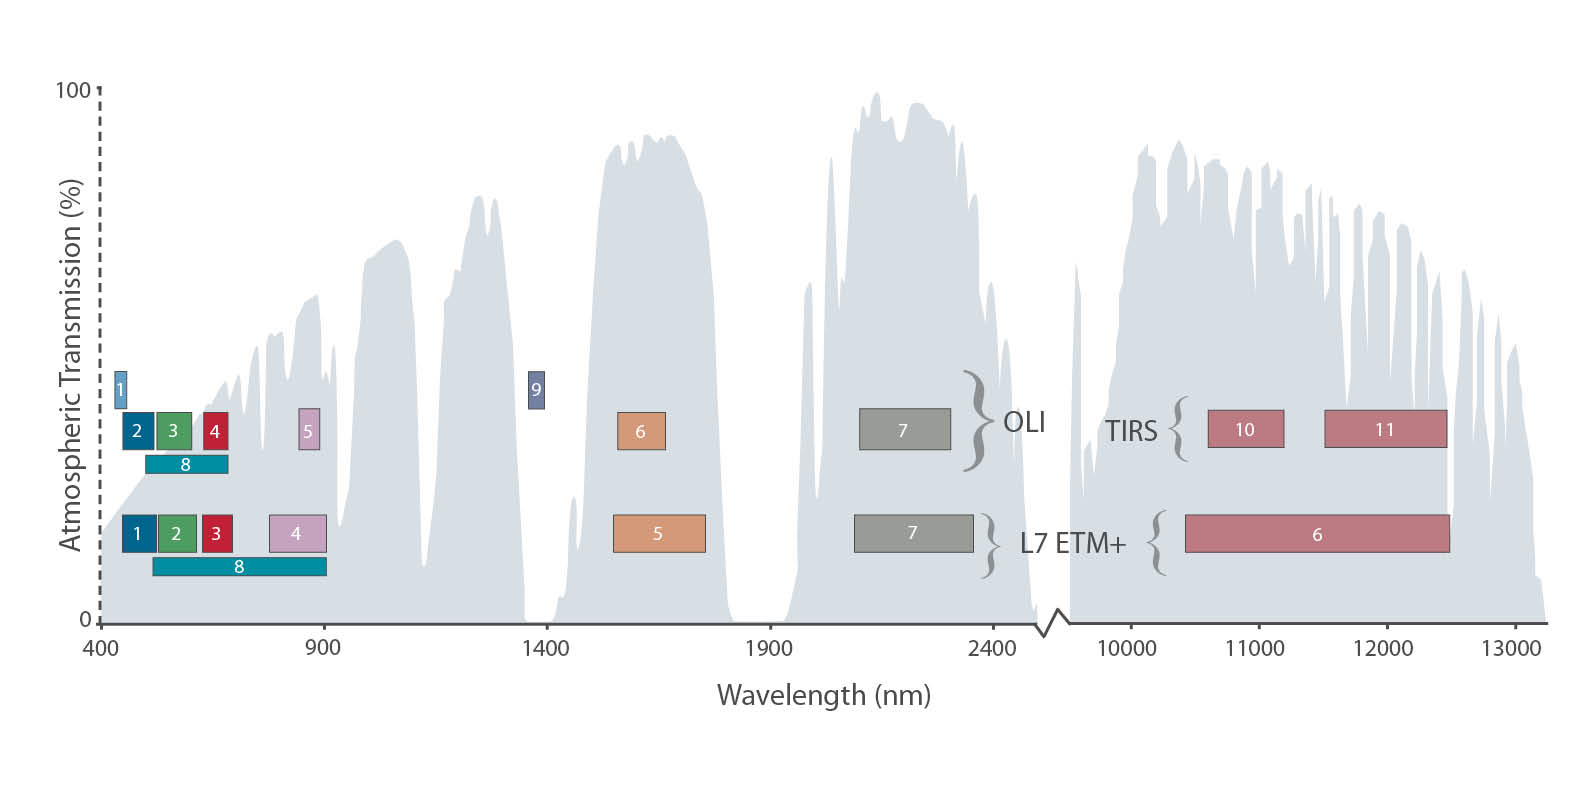
\includegraphics[scale=0.13]{images/bands/landsat8_bands.jpg}
\end{overlayarea}
\begin{overlayarea}{\linewidth}{1cm}
  \centering
  \scriptsize \href{http://landsat.gsfc.nasa.gov/sentinel-2a-launches-our-compliments-our-complements/}{Landsat-8 bands (OLI/TIRS sensors)}\par
\end{overlayarea}
\end{column}
\end{columns}
\end{frame}

\section{Importing labels}

\subsection{Importing densities}
\begin{frame}
 \begin{itemize}
  \item Take cities surfaces and densities from 2013 official census (\href{http://www.insee.fr/fr/ppp/bases-de-donnees/recensement/populations-legales/pages2015/zip/HIST_POP_COM_RP13.zip}{INSEE})
  \item Take cities latitude and longitude from Google geolocator (\href{https://geopy.readthedocs.io/en/1.10.0/}{Python API Geopy})
 \end{itemize}

\begin{columns}
\begin{column}{0.80\textwidth}
\begin{overlayarea}{\linewidth}{3cm}
\begin{table}
\begin{center}
\begin{adjustbox}{max width=\textwidth}
{\LARGE
\begin{tabular}{|c|c|c|c|c|}
\hline 
name & latitude (degrees) & longitude (degrees) & surface (km\textsuperscript{2}) & density (habs/km\textsuperscript{2}) \\
\hline
Ozan & 46.391534 & 4.915265 & 6.6 & 98.3\\
\hline 
Cormoranche-sur-Sa\^{o}ne & 46.240532 & 4.830863 & 9 & 118.9\\
\hline 
Paris & 48.856614 & 2.352222 & 105.4 & 21153.9\\
\hline
Lyon & 45.764043 & 4.835659 & 47.87 & 10117.0\\
\hline
Tours & 47.394144 & 0.68484 & 34.67 & 3888.2\\
\hline
Besancon & 47.237829 & 6.024054 & 65.05 & 1797.9\\
\hline 
... & ... & ... & ... & ... \\
\hline
\end{tabular}
}
\end{adjustbox}
\end{center}
\end{table}
\end{overlayarea}
\begin{overlayarea}{\linewidth}{1cm}
  \centering
  \scriptsize34190 cities (instances)\par
\end{overlayarea}
\end{column}
\end{columns}

\end{frame}

\subsection{Categorize densities to Classification}
\begin{frame}
\begin{itemize}
 \item Categorize densities applying clustering (Otsu mutli-thresholding)
\end{itemize}

\begin{columns}
 \begin{column}{0.50\textwidth}
  \begin{overlayarea}{\linewidth}{3cm}
  \centering\vfill
  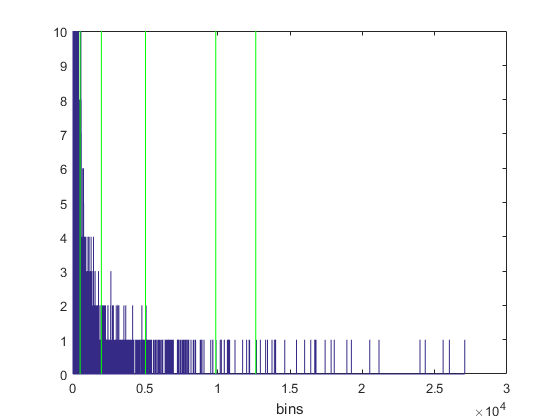
\includegraphics[scale=0.25]{images/labels/densite_histo_otsu_zoom.png}
  \end{overlayarea}
  \begin{overlayarea}{\linewidth}{0.5cm}
  \centering
  \tiny Density histogram (habs/km\textsuperscript{2})\par
  \end{overlayarea}
 \end{column}
 \begin{column}{0.50\textwidth}
  \begin{overlayarea}{\linewidth}{3cm}
  {\tiny
    \begin{itemize}
    \item[catégory 1:] density between 0 and 500 habs/km\textsuperscript{2}
    \item[catégory 2:] density between 500 and 2000 habs/km\textsuperscript{2}
    \item[catégory 3:] density between 2000 and 5000 habs/km\textsuperscript{2}
    \item[catégory 4:] density between 5000 and 10000 habs/km\textsuperscript{2}
    \item[catégory 5:] density between 10000 and 13000 habs/km\textsuperscript{2}
    \item[catégory 6:] density greater than 13000 habs/km\textsuperscript{2}
    \end{itemize}
  }
  \end{overlayarea}
 \end{column}
\end{columns}

\begin{table}
\begin{center}
\begin{adjustbox}{max width=\textwidth}
{\tiny
\begin{tabular}{|c|c|c|c|c|c|}
\hline 
city & latitude (degrees) & longitude (degrees) & surface (km\textsuperscript{2}) & density (habs/km\textsuperscript{2}) & density (category)\\
\hline
Ozan & 46.391534 & 4.915265 & 6.6 & 98.3 & 1\\
\hline 
Cormoranche-sur-saone & 46.240532 & 4.830863 & 9 & 118.9 & 1\\
\hline 
Paris & 48.856614 & 2.352222 & 105.4 & 21153.9 & 6\\
\hline
Lyon & 45.764043 & 4.835659 & 47.87 & 10117.0 & 5\\
\hline
Tours & 47.394144 & 0.68484 & 34.67 & 3888.2 & 3\\
\hline
Besancon & 47.237829 & 6.024054 & 65.05 & 1797.9 & 1\\
\hline 
... & ... & ... & ... & ... & ...\\
\hline
\end{tabular}
}
\end{adjustbox}
\end{center}
\end{table}

\end{frame}

\section{Vegetation index extraction}

\subsection{NDVI extraction}
\begin{frame}
\begin{itemize}
{
 \item Compute Normalized Difference Vegetation Indice using bands 4 (Red) and 5 (Near-Infra-Red) for each dataset :
 \item Values between -1 and 1
 \item $\leq 0$ for water, snow and cloud
 \item $= 0$ for  ground without vegetation
 \item $\geq 0$ for ground vegetation
}
\end{itemize}
{\scriptsize \[NDVI=\frac{NIR-R}{NIR+R}\]}
\begin{columns}
 \begin{column}{0.33\textwidth}
  \begin{overlayarea}{\linewidth}{2cm}
  \centering\vfill
  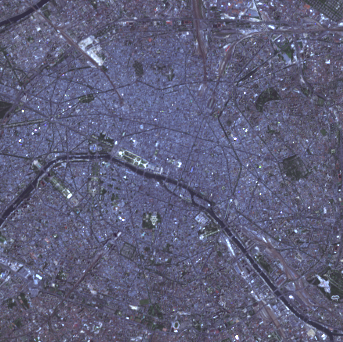
\includegraphics[scale=0.15]{images/Paris/05_rgb.png}
  \end{overlayarea}
  \begin{overlayarea}{\linewidth}{0.5cm}
  \centering
  \tiny RGB (Paris,May 2013) \par
  \end{overlayarea}
 \end{column}
  \begin{column}{0.33\textwidth}
  \begin{overlayarea}{\linewidth}{2cm}
  \centering\vfill
  \centerline{
  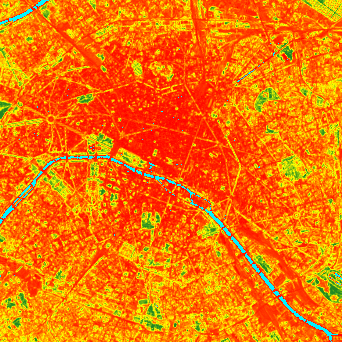
\includegraphics[scale=0.15]{images/Paris/05_ndvi.png}
  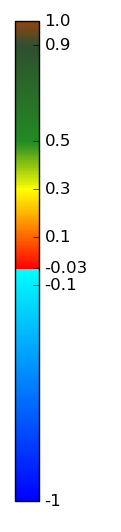
\includegraphics[scale=0.13]{images/colormap.png}
  }
  \end{overlayarea}
  \begin{overlayarea}{\linewidth}{0.5cm}
  \centering
  \tiny NDVI (Paris,May 2013) \par
  \end{overlayarea}
 \end{column}
 \begin{column}{0.33\textwidth}
  \begin{overlayarea}{\linewidth}{2cm}
  \centering\vfill
  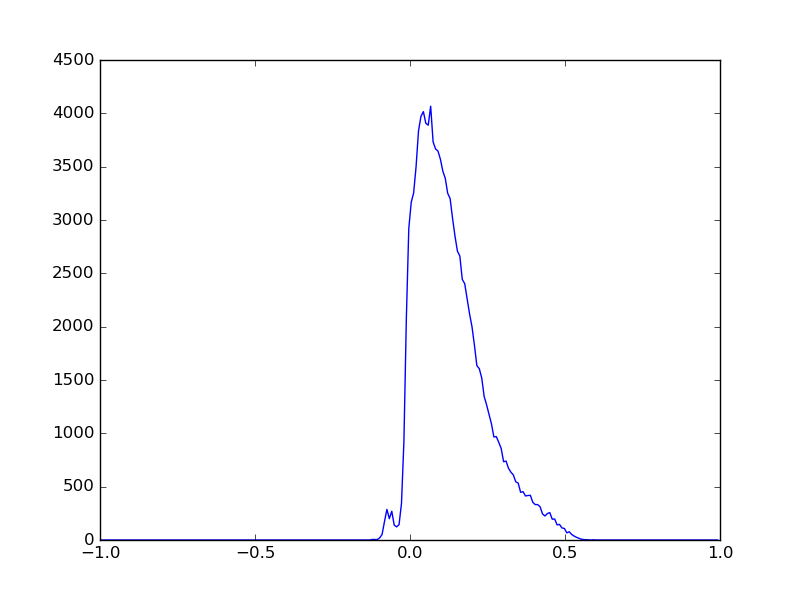
\includegraphics[scale=0.12]{images/Paris/05_ndvi_histo.png}
  \end{overlayarea}
  \begin{overlayarea}{\linewidth}{0.5cm}
  \centering
  \tiny NDVI (1024 bins)-histogram (Paris,May 2013) \par
  \end{overlayarea}
 \end{column}
\end{columns}

\end{frame}

\subsection{NDVI evolution}
\begin{frame}

\begin{columns}
 \begin{column}{0.75\textwidth}
 
 \begin{overlayarea}{\linewidth}{2cm}
 \begin{itemize}
 \item NDVI histogram could explain human density
 \begin{itemize}
  \item \scriptsize low ndvi mode for high density (poor vegetation)
  \item \scriptsize high ndvi mode for low density (rich vegetation)
 \end{itemize}
 \end{itemize}
 \end{overlayarea}

  \begin{overlayarea}{\linewidth}{4.5cm}
  \centering\vfill
  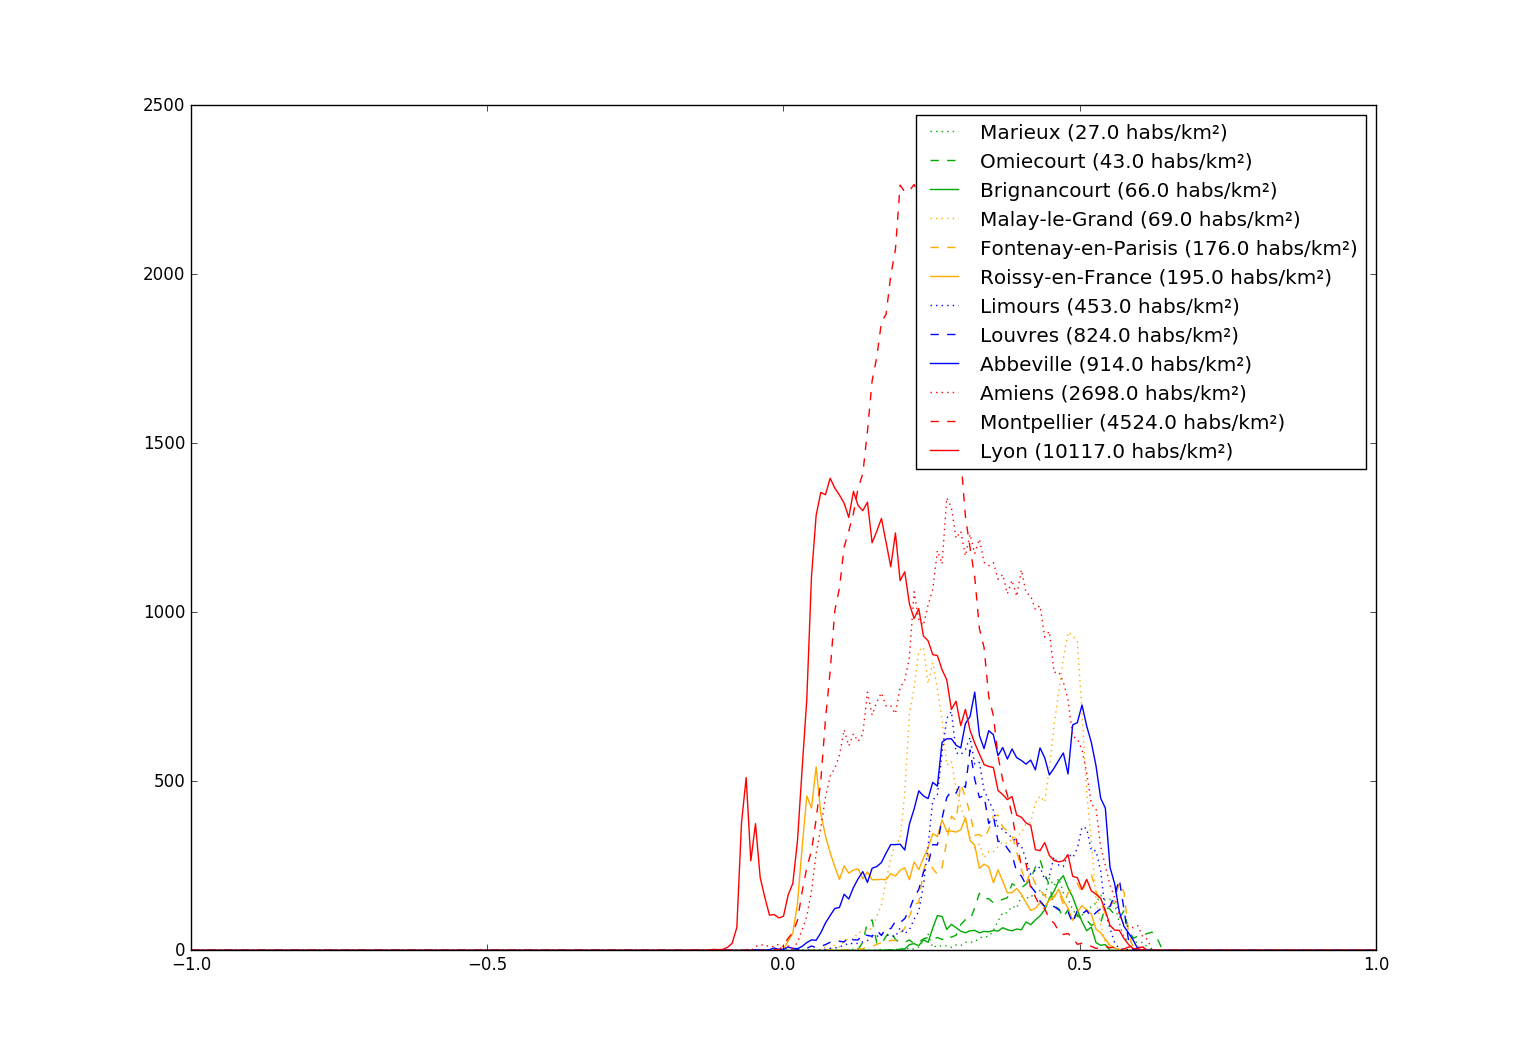
\includegraphics[scale=0.17]{images/ndvi/ndvi_categorie.png}
  \end{overlayarea}
  \begin{overlayarea}{\linewidth}{0.5cm}
  \centering
  \tiny NDVI (1024 bins)-histograms (French cities, July 2013) \par
  \end{overlayarea}
  
 \end{column}
 \begin{column}{0.25\textwidth}
 
 \begin{overlayarea}{\linewidth}{0.5cm}
  \centering\vfill
  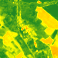
\includegraphics[scale=0.17]{images/Brignancourt/07_ndvi.png}
  \end{overlayarea}
  \begin{overlayarea}{\linewidth}{0.5cm}
  \centering
  \tiny NDVI - Brignancourt (66 habs/km\textsuperscript{2}) - July 2013) \par
  \end{overlayarea}
  
  \begin{overlayarea}{\linewidth}{0.9cm}
  \centering\vfill
  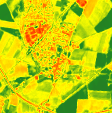
\includegraphics[scale=0.17]{images/Louvres/07_ndvi.png}
  \end{overlayarea}
  \begin{overlayarea}{\linewidth}{0.5cm}
  \centering
  \tiny NDVI - Louvres (824 habs/km\textsuperscript{2}) - July 2013) \par
  \end{overlayarea}
  
  \begin{overlayarea}{\linewidth}{1.2cm}
  \centering\vfill
  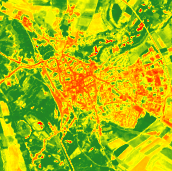
\includegraphics[scale=0.17]{images/Abbeville/07_ndvi.png}
  \end{overlayarea}
  \begin{overlayarea}{\linewidth}{0.5cm}
  \centering
  \tiny NDVI - Abbeville (914 habs/km\textsuperscript{2}) - July 2013 \par
  \end{overlayarea}
  
  \begin{overlayarea}{\linewidth}{1.6cm}
  \centering\vfill
  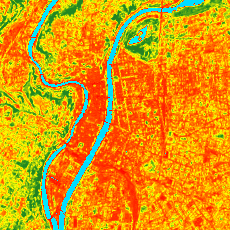
\includegraphics[scale=0.17]{images/Lyon/07_ndvi.png}
  \end{overlayarea}
  \begin{overlayarea}{\linewidth}{0.5cm}
  \centering
  \tiny NDVI - Lyon (10117 habs/km\textsuperscript{2}) - July 2013) \par
  \end{overlayarea}  
 \end{column}

\end{columns}


\end{frame}

\subsection{Data to Machine Learning}
\begin{frame}
 \begin{itemize}
  \item Explanatory variables : NDVI (1024 bins)-histograms of the 34190 cities
  \item Predictable variable : density of the 34190 cities for regresion
  \item Predictable variable : density category of the 34190 cities for classification
 \end{itemize}
 
\begin{columns}
\begin{column}{0.8\textwidth}
\begin{table}
\begin{center}
\begin{adjustbox}{max width=0.9\textwidth}
\begin{tabular}{|c|c|c|c|c|c|c|c|c|c|c|}

\hline 
city &  bin-1 & bin-2 & ... & bin-511 & bin-512 &... & bin-1023 & bin-1024 & density (habs/km\textsuperscript{2})  & density (category)\\
\hline 
Ozan & 0 & 0 & ... & 1 & 5 & ... & 0 & 0 & 93.8 & 1\\
\hline 
Cormoranche-sur-Sa\^{o}ne & 0 & 0 & ... & 1 & 4 & ... & 0 & 0 & 118.9 & 1\\
\hline 
Paris & 0 & 0 & ... & 1953 & 1815 & ... & 0 & 0 & 21153.9 & 6\\
\hline
Lyon & 0 & 0 & ... & 1099 & 1032 & ... & 0 & 0 & 10117.0 & 5\\
\hline
Tours & 0 & 0 & ... & 268 & 238 & ... & 0 & 0 & 3888.2 & 3\\
\hline
Besancon & 0 & 0 & ... & 97 & 122 & ... & 0 & 0 & 1797.9 & 1\\
\hline 
... & ... & ... & ... & ... & ... & ... & ... & ... & ... & ... \\
\hline
\end{tabular}
\end{adjustbox}
\end{center}
\end{table}
\end{column}
\begin{column}{0.35\textwidth}
{\tiny
\begin{alertblock}{Very imbalanced data for classification!}
\begin{table}
 \begin{tabular}{|c|c|}
  \hline
  category & number of samples\\
  \hline
  \textbf{1} & 32533\\
  \hline
  \textbf{2} & 1252\\
  \hline
  \textbf{3} & 288\\
  \hline
  \textbf{4} & 78\\
  \hline
  \textbf{5} & 15\\
  \hline
  \textbf{6} & 24 \\
  \hline
 \end{tabular}
\end{table}
\end{alertblock}
}
\end{column}
\end{columns}
\end{frame}

\section{Supervised Classification}

\subsection{K-Nearest Neighbors}
\begin{frame}
\begin{itemize}
 \item Overcome imbalanced data by 
  \begin{itemize}
  {\scriptsize
    \item Oversampling minority classes using SMOTE technique (Synthetic Minority Oversampling TEchnique) 
      \begin{columns}
      \begin{column}{0.5\textwidth}
      \centering\vfill
      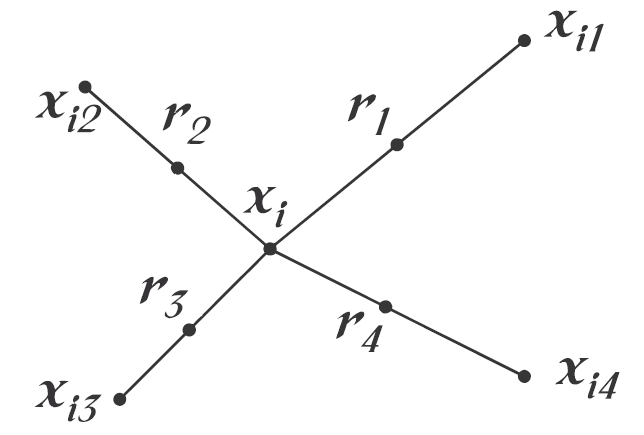
\includegraphics[scale=0.17]{images/oversampling/smote.png}
      \end{column}
      \begin{column}{0.5\textwidth}
      {\tiny
      Let's $x_{i}$,$x_{i1}$, $x_{i2}$, $x_{i3}$ and $x_{i4}$ be points of minority class $i$ and $y_{jk}$ the points of 
      majority class $j$ , choose each new sample $r_{l}$ for class $i$ that maximizes $\sum \limits_{\underset{}{k=1}}^{n_{j}} (y_{jk}-r_{l})^2$
      }
      \end{column}
    \end{columns}
    \item Run training on obtained balanced data.
  }
  \end{itemize}
 \end{itemize}
 \begin{itemize}
  \item Best cross-validation (stratified 3-folds) of \textbf{$94.74$\%} obtained for number of neighboors $k = 5$. 
 \end{itemize}
\end{frame}

\begin{frame}
\begin{columns}
 \begin{column}{0.5\textwidth}
  \begin{overlayarea}{\linewidth}{4cm}
    \centering\vfill
    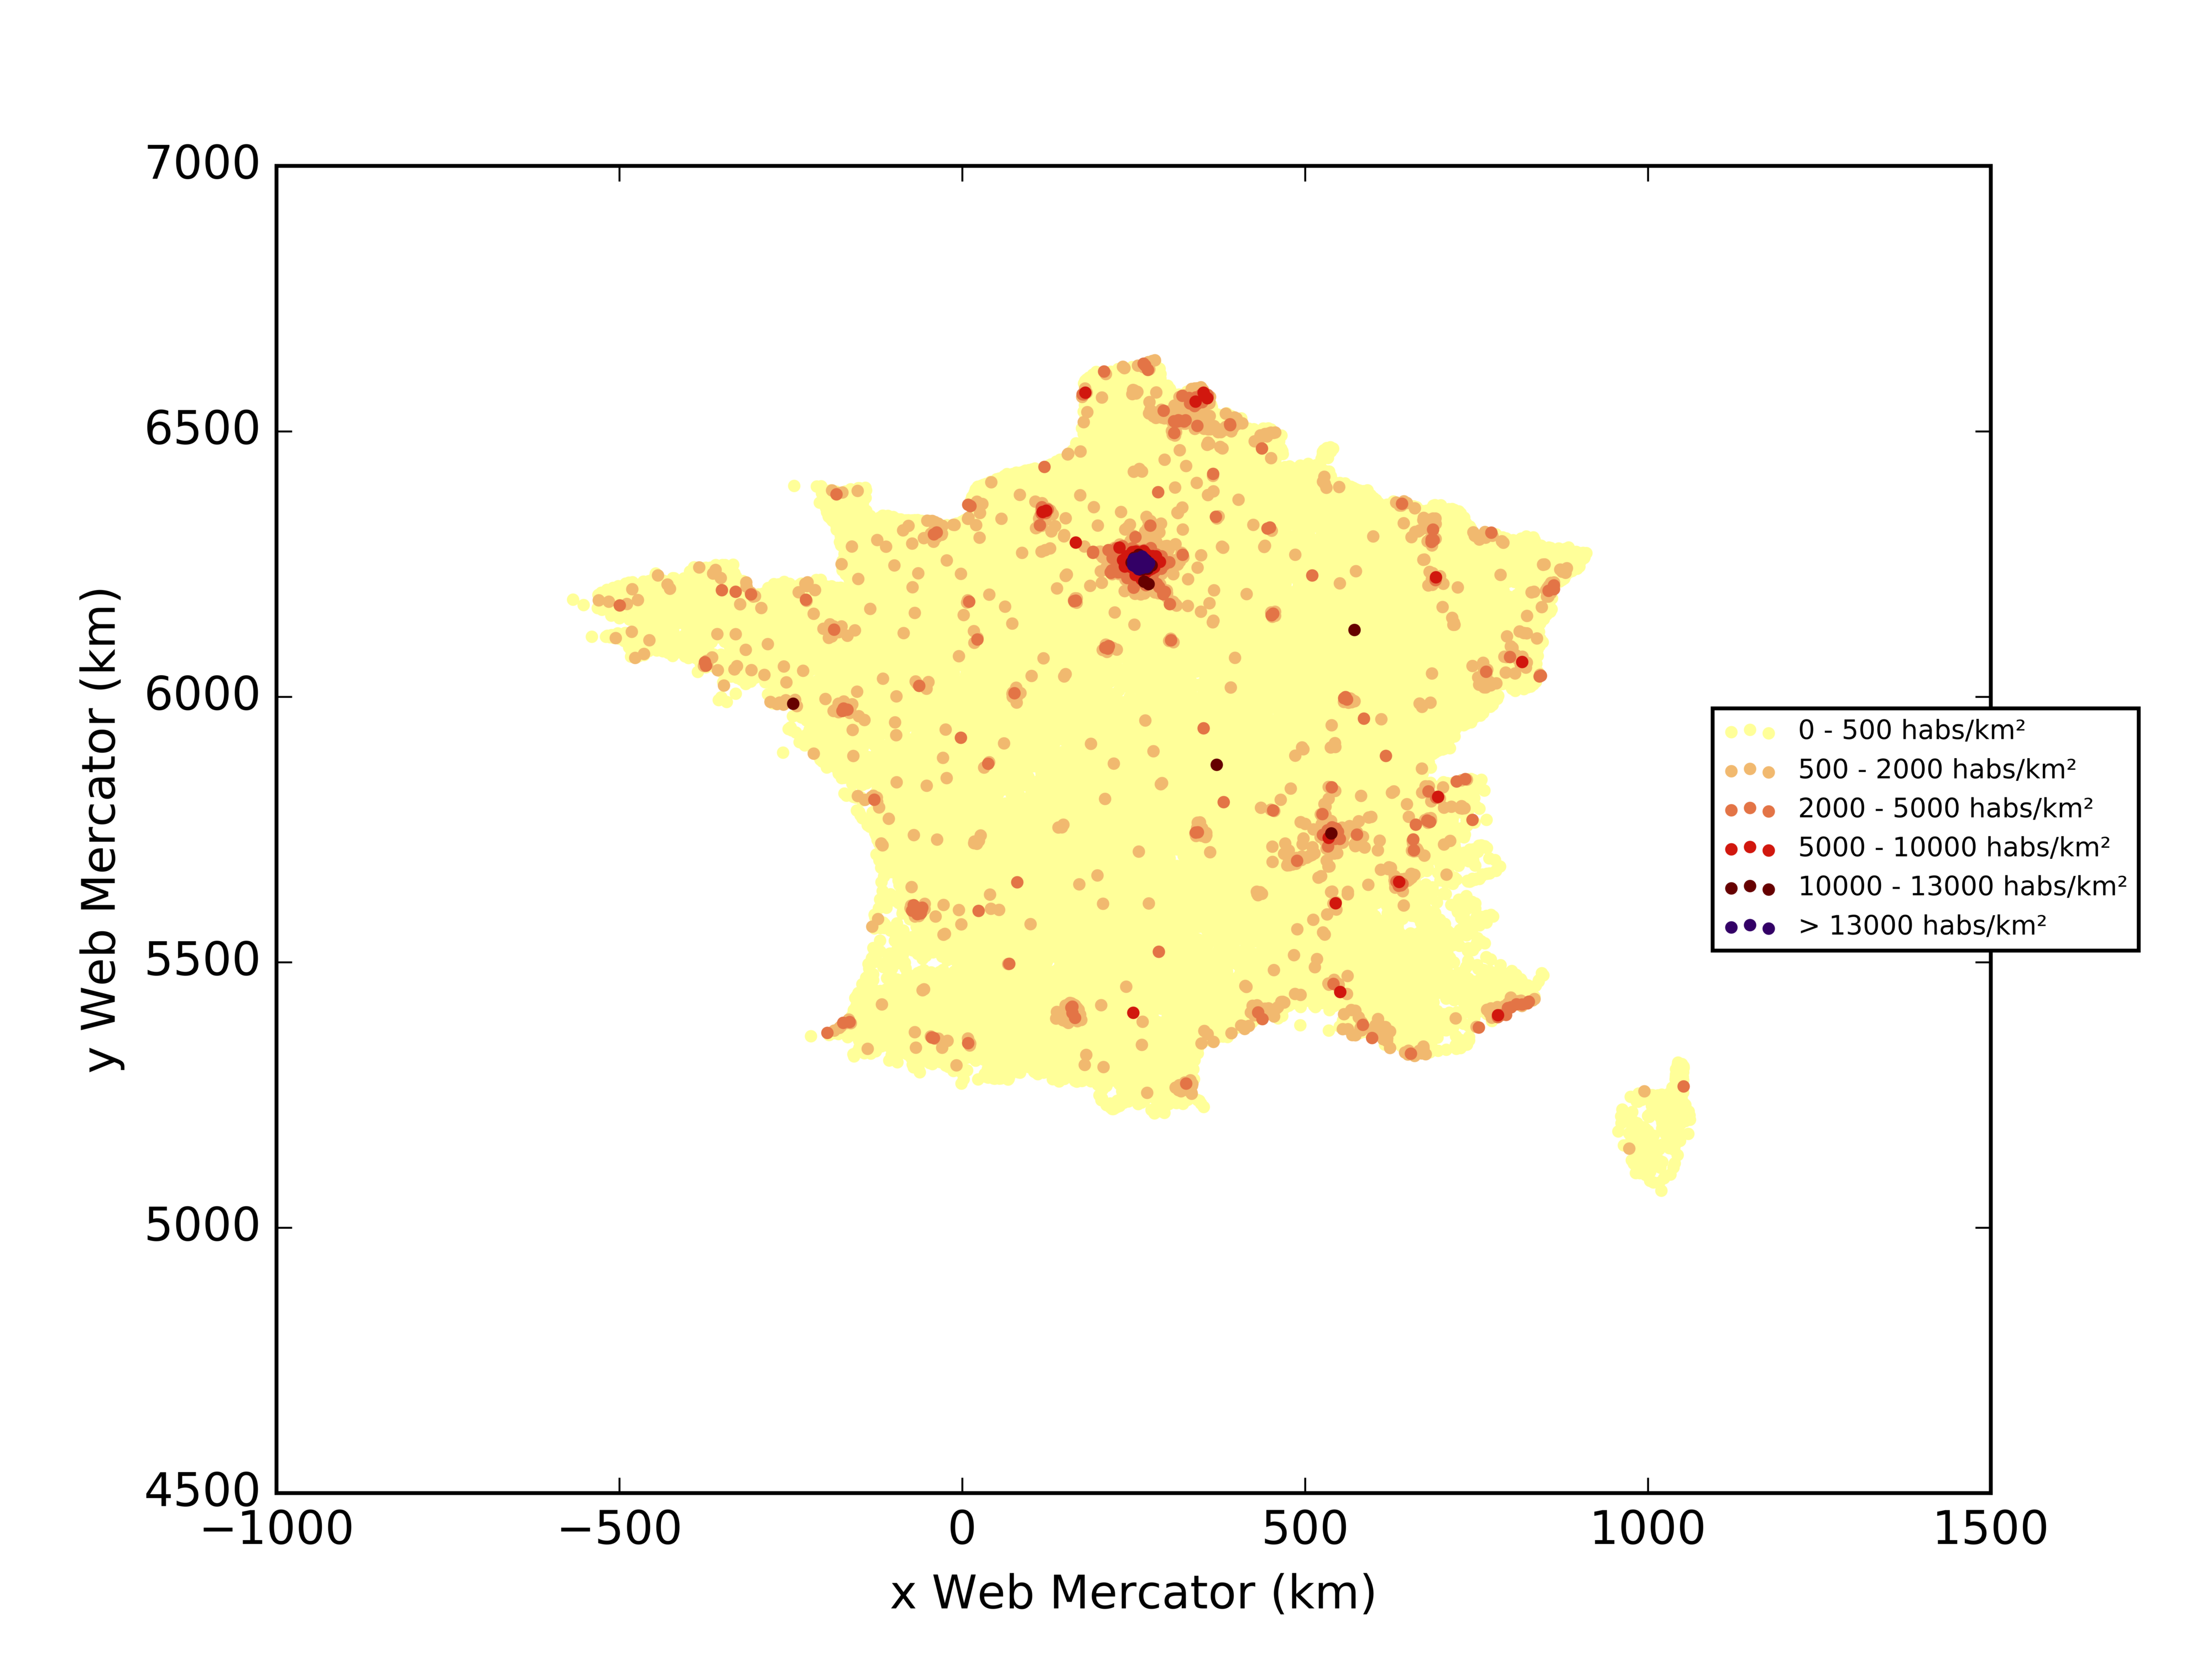
\includegraphics[scale=0.50]{images/France/density_ground_truth.png}
  \end{overlayarea}
  \begin{overlayarea}{\linewidth}{0.5cm}
    \centering
    \tiny France density category - ground truth\par
  \end{overlayarea}
 \end{column}
 \begin{column}{0.5\textwidth}
  \begin{overlayarea}{\linewidth}{4cm}
    \centering\vfill
    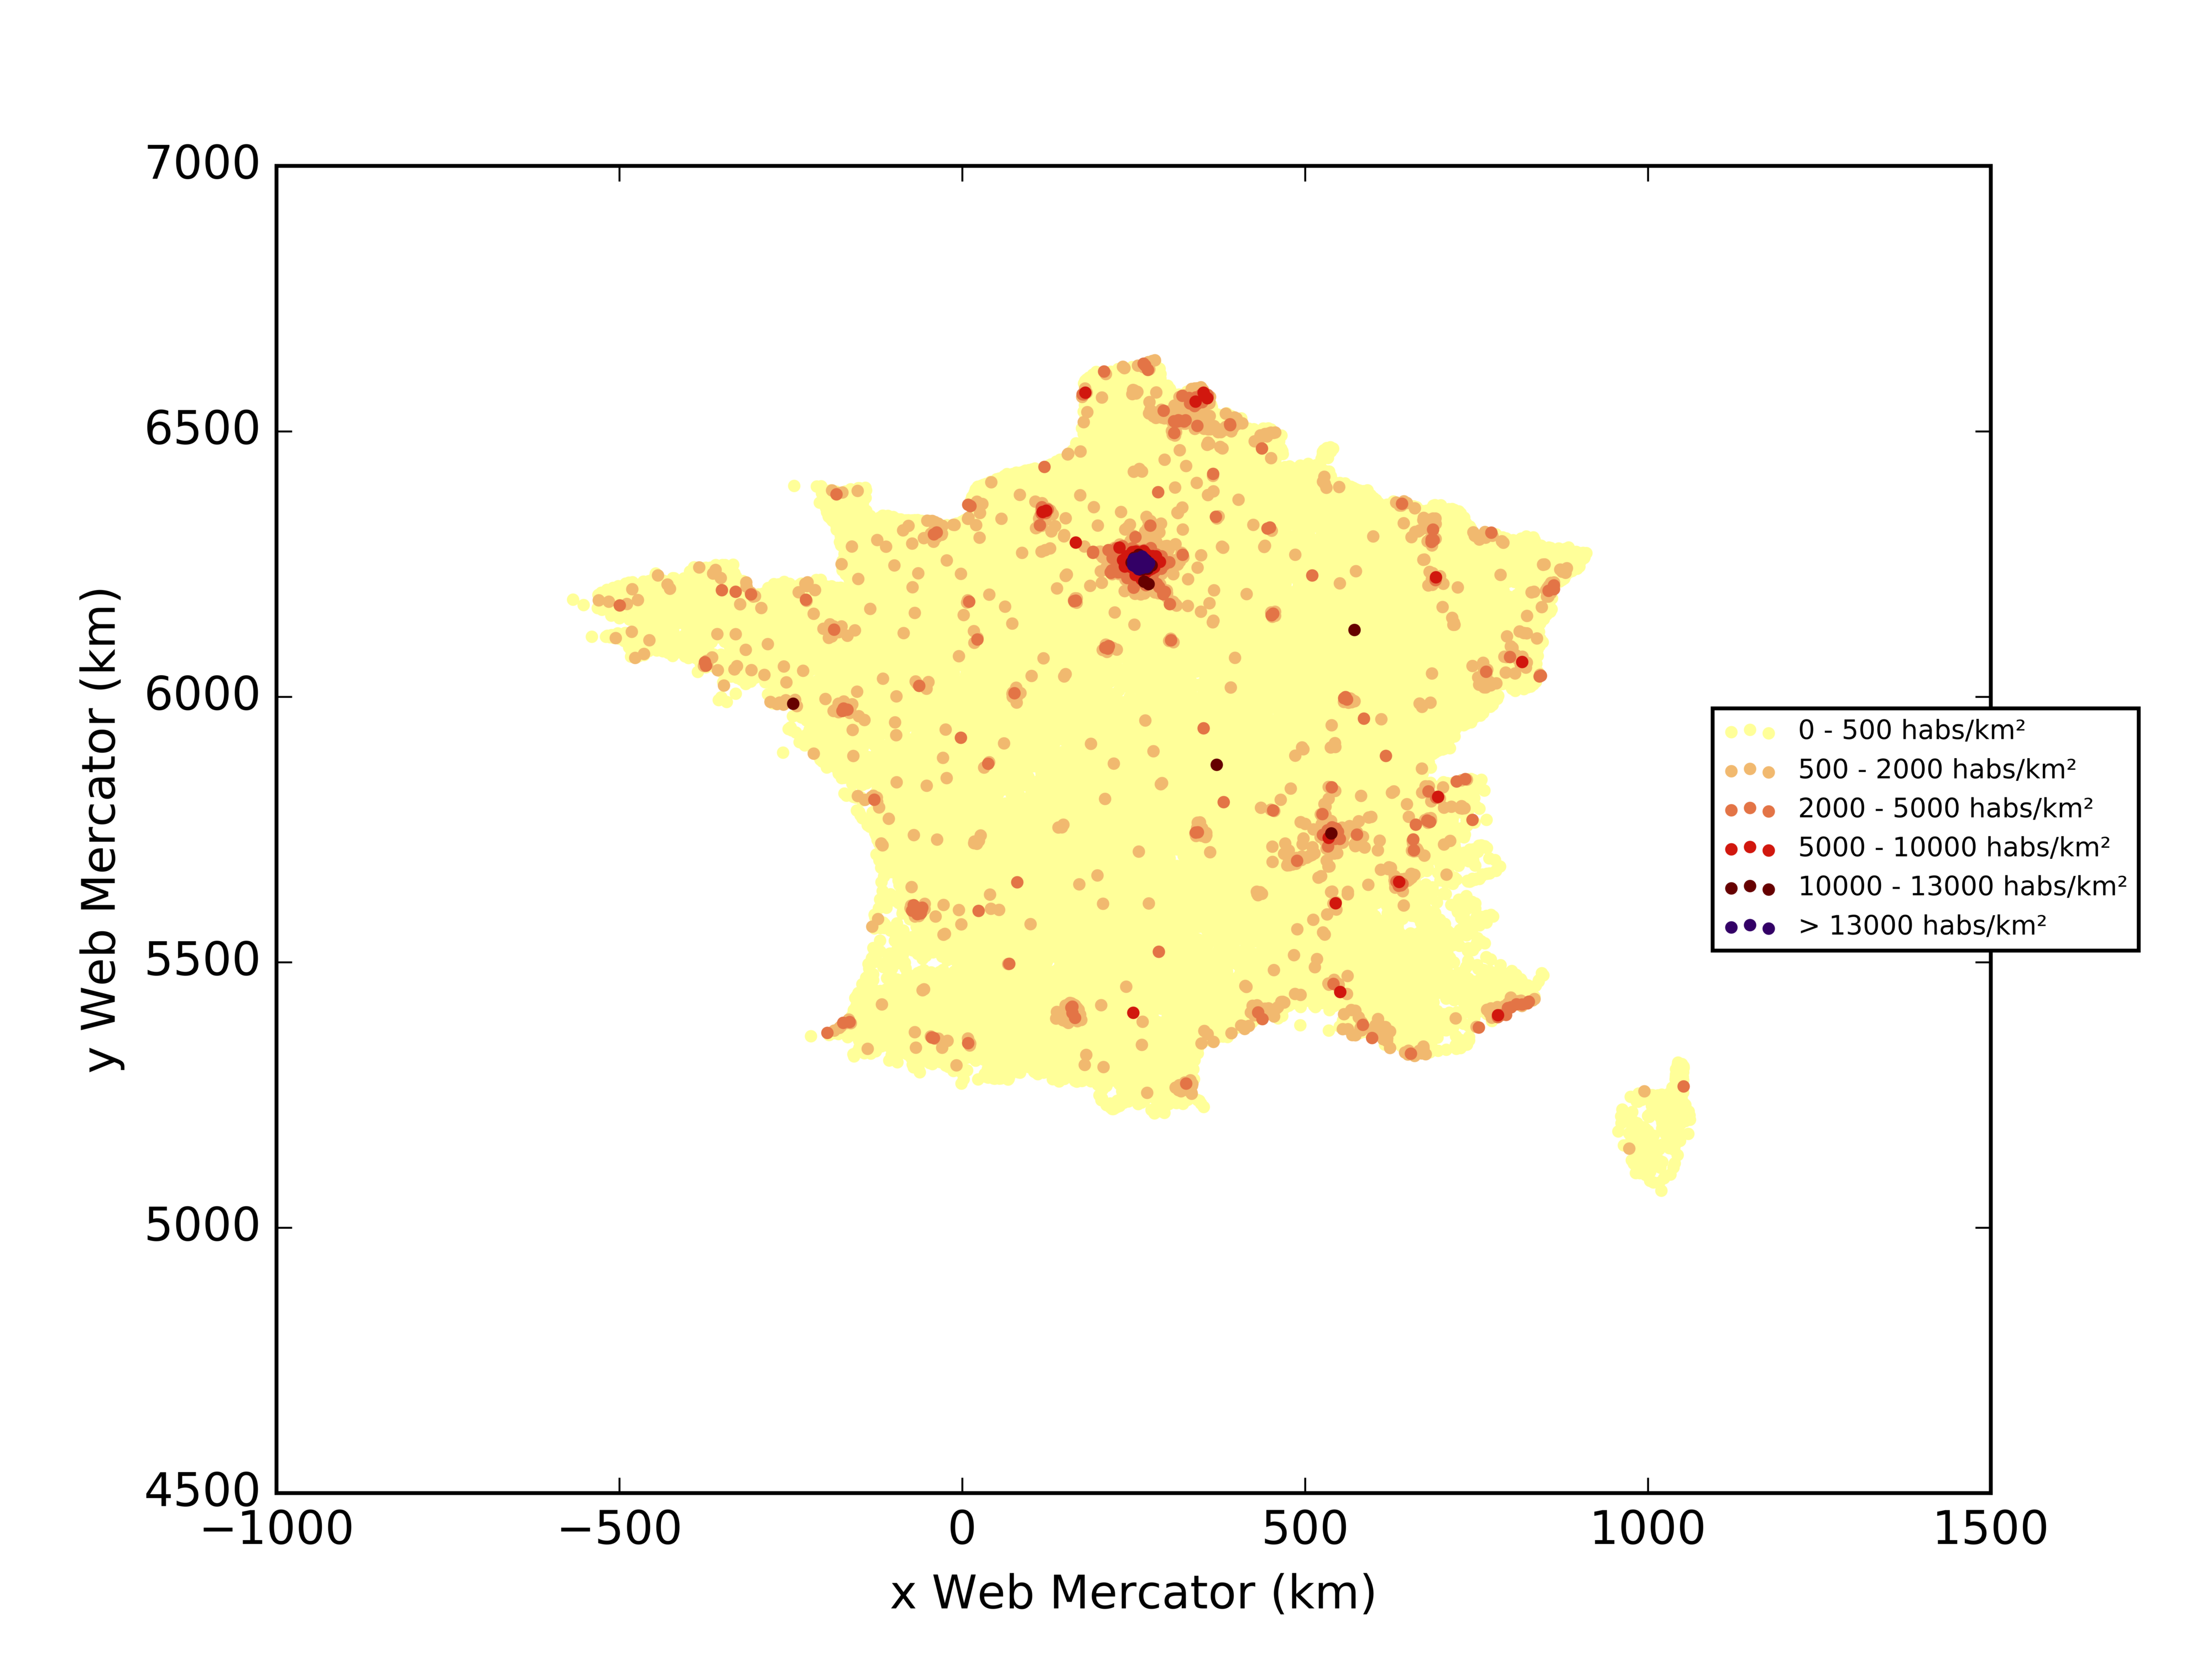
\includegraphics[scale=0.50]{images/France/knn/density_classification.png}
  \end{overlayarea}
  \begin{overlayarea}{\linewidth}{0.5cm}
    \centering
    \tiny France density category - prediction\par
  \end{overlayarea}
 \end{column}
\end{columns}

\begin{columns}
\begin{column}{0.7\textwidth}
  \begin{table}
  \begin{center}
  \begin{adjustbox}{max width=0.6\textwidth}
  {\tiny
  \begin{tabular}{|c|c|c|c|c|c|c|}
    \hline
    \multicolumn{7}{|c|}{{\tiny \begin{bf}Confusion matrix after refitting\end{bf}}} \\
    \hline
     & \textbf{1} & \textbf{2} & \textbf{3} & \textbf{4} & \textbf{5} & \textbf{6}\\
    \hline
    \textbf{1} & 32533 & 0 & 0 & 0 & 0 & 0\\
    \hline
    \textbf{2} & 0 & 1252 & 0 & 0 & 0 & 0\\
    \hline
    \textbf{3} & 0 & 0 & 288 & 0 & 0 & 0\\
    \hline
    \textbf{4} & 0 & 0 & 0 & 78 & 0 & 0\\
    \hline
    \textbf{5} & 0 & 0 & 0 & 0 & 15 & 0\\
    \hline
    \textbf{6} & 0 & 0 & 0 & 0 & 0 & 24\\
    \hline
  \end{tabular}
  }
  \end{adjustbox}
  \end{center}
  \end{table}
\end{column}
\begin{column}{0.5\textwidth}
   \begin{table}
    \begin{center}
    \begin{adjustbox}{max width=0.5\textwidth}
    {\tiny 
    \begin{tabular}{|c|c|}
      \hline
      \multicolumn{2}{|c|}{\begin{bf}Mean score per class after reffiting\end{bf}} \\
      \hline
      \textbf{category} & \textbf{mean score}\\
      \hline
      \textbf{1} & 100\% \\
      \hline
      \textbf{2} & 100\% \\
      \hline
      \textbf{3} & 100\% \\
      \hline
      \textbf{4} & 100\% \\
      \hline
      \textbf{5} & 100\% \\
      \hline
      \textbf{6} & 100\% \\
      \hline
      \textbf{mean} & 100\% \\
      \hline
    \end{tabular}
    }
    \end{adjustbox}
    \end{center}
  \end{table}
\end{column}

\end{columns}
\end{frame}

\subsection{Neural Network}

\begin{frame}
\begin{itemize}
 \item Overcome imbalanced data by 
  \begin{itemize}
  {\scriptsize
    \item Majoring error by weights to penalize error on minority class, during back-propagation : $w_i=\frac{n_1}{n_i}$.
  }
  \end{itemize}
 \end{itemize}
 \begin{itemize}
  \item Best cross-validation (stratified 3-folds) of \textbf{$92.26$\%} with SGD learning rate of $0.001$ and penalization of $0.001$. 
 \end{itemize}
\end{frame}

\begin{frame}
\begin{columns}
 \begin{column}{0.5\textwidth}
  \begin{overlayarea}{\linewidth}{4cm}
    \centering\vfill
    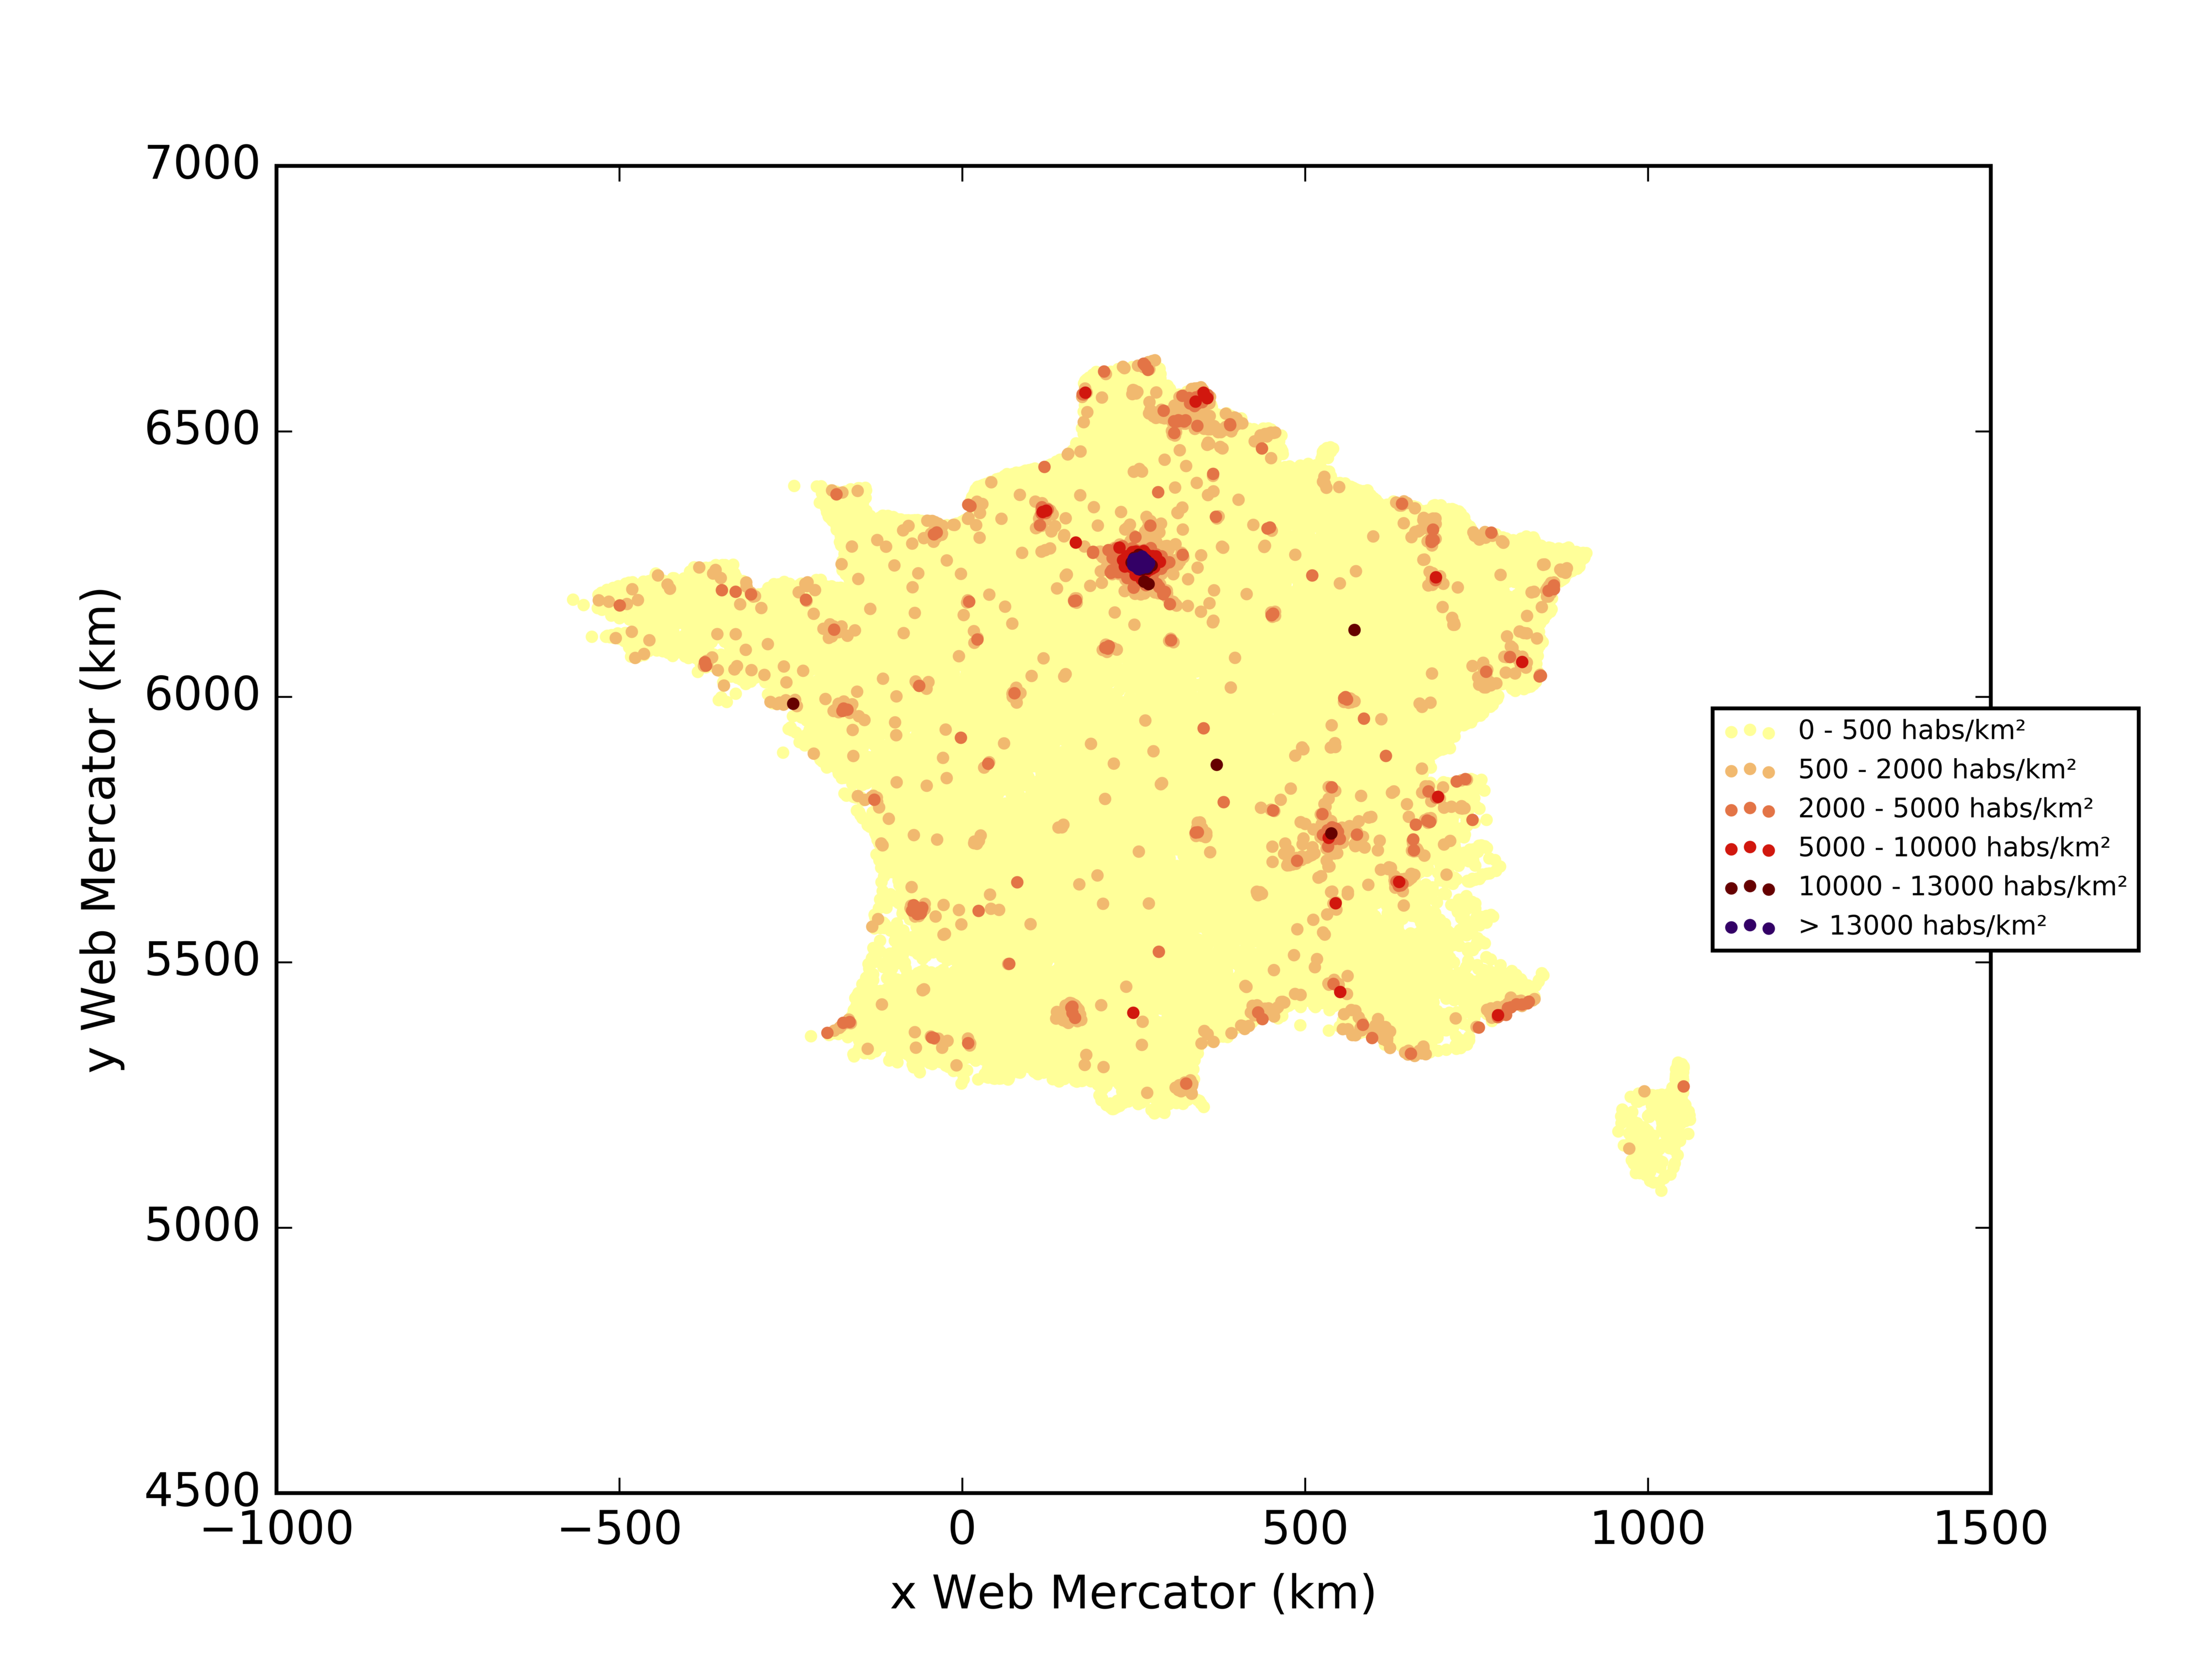
\includegraphics[scale=0.50]{images/France/density_ground_truth.png}
  \end{overlayarea}
  \begin{overlayarea}{\linewidth}{0.5cm}
    \centering
    \tiny France density category - ground truth\par
  \end{overlayarea}
 \end{column}
 \begin{column}{0.5\textwidth}
  \begin{overlayarea}{\linewidth}{4cm}
    \centering\vfill
    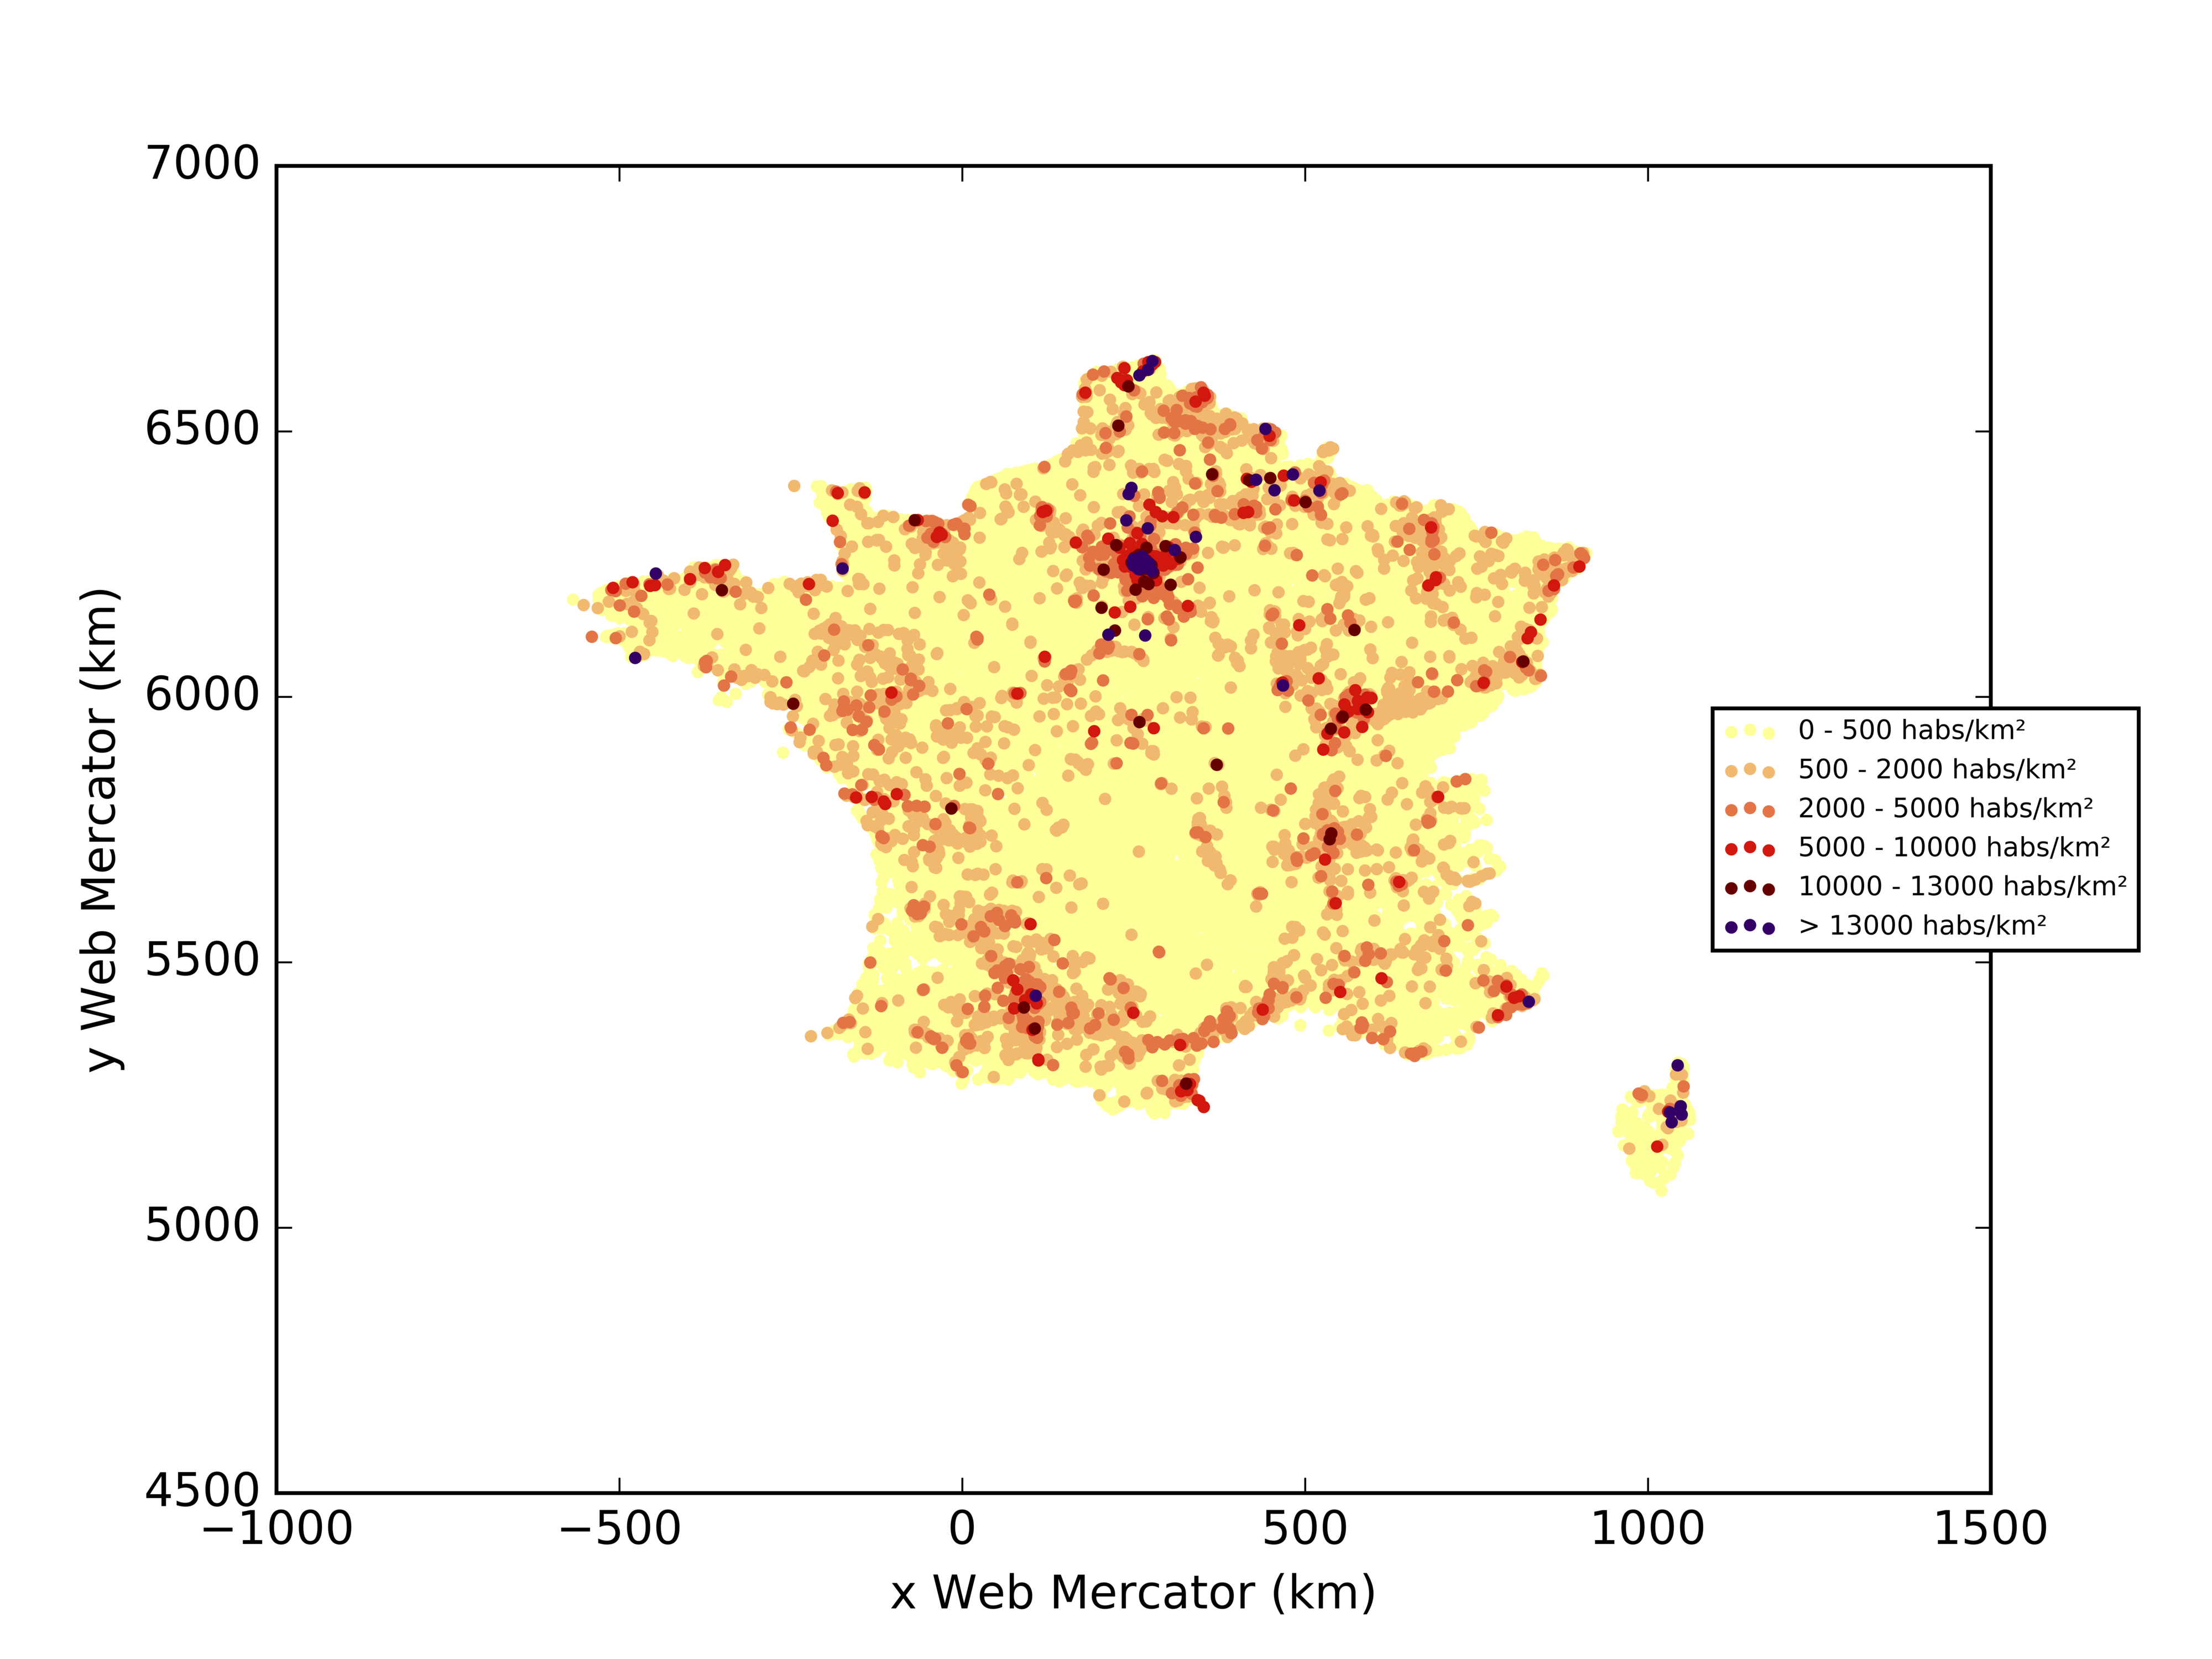
\includegraphics[scale=0.50]{images/France/nn/density_classification.png}
  \end{overlayarea}
  \begin{overlayarea}{\linewidth}{0.5cm}
    \centering
    \tiny France density category - prediction\par
  \end{overlayarea}
 \end{column}
\end{columns}

\begin{columns}
\begin{column}{0.7\textwidth}
  \begin{table}
  \begin{center}
  \begin{adjustbox}{max width=0.6\textwidth}
  {\tiny
  \begin{tabular}{|c|c|c|c|c|c|c|}
    \hline
    \multicolumn{7}{|c|}{{\tiny \begin{bf}Confusion matrix after refitting\end{bf}}} \\
    \hline
     & \textbf{1} & \textbf{2} & \textbf{3} & \textbf{4} & \textbf{5} & \textbf{6}\\
    \hline
    \textbf{1} & 29743 & 2281 & 367 & 95 & 24 & 23\\
    \hline
    \textbf{2} & 207 & 853 & 164 & 23 & 2 & 3\\
    \hline
    \textbf{3} & 2 & 36 & 236 & 9 & 2 & 3\\
    \hline
    \textbf{4} & 0 & 0 & 2 & 76 & 0 & 0\\
    \hline
    \textbf{5} & 0 & 0 & 0 & 0 & 15 & 0\\
    \hline
    \textbf{6} & 0 & 0 & 0 & 0 & 0 & 24\\
    \hline
  \end{tabular}
  }
  \end{adjustbox}
  \end{center}
  \end{table}
\end{column}
\begin{column}{0.5\textwidth}
   \begin{table}
    \begin{center}
    \begin{adjustbox}{max width=0.5\textwidth}
    {\tiny 
    \begin{tabular}{|c|c|}
      \hline
      \multicolumn{2}{|c|}{\begin{bf}Mean score per class after reffiting\end{bf}} \\
      \hline
      \textbf{category} & \textbf{mean score}\\
      \hline
      \textbf{1} & 91.42\% \\
      \hline
      \textbf{2} & 68.13\% \\
      \hline
      \textbf{3} & 91.95\% \\
      \hline
      \textbf{4} & 97.64\% \\
      \hline
      \textbf{5} & 100\% \\
      \hline
      \textbf{6} & 100\% \\
      \hline
      \textbf{mean} & 89.82\% \\
      \hline
    \end{tabular}
    }
    \end{adjustbox}
    \end{center}
  \end{table}
\end{column}
\end{columns}
\end{frame}

\subsection{Support-Vector Machine (Gaussian Kernel)}
\begin{frame}
\begin{itemize}
 \item Overcome imbalanced data by increasing regularization parameter $C_{i}$ for minority classes $i$ :  $C_{i} = 10000/n_{i}$
 \item Cross-validated (stratified 5-folds) gamma coefficient ($\gamma = 0.001$)
\end{itemize}
\end{frame}

\subsection{Convolutional Neural Network}
\begin{frame}

\end{frame}

\section{Testing classification}

\subsection{Data}
\begin{frame}
\begin{itemize}
{\scriptsize
 \item Take ground truth densities and surfaces for \href{https://www.bfs.admin.ch/bfs/fr/home/statistiques/population/effectif-evolution/population.assetdetail.1401563.html}{Switzerland} (2013),
  \href{https://fr.wikipedia.org/wiki/Liste_des_communes_de_Belgique_par_population}{Belgium} (2015)  and \href{https://www.citypopulation.de/php/netherlands-admin.php}{Netherlands} (2014).
 \begin{columns}
  \begin{column}{0.33\textwidth}
   \begin{table}
   \begin{center}
   \begin{adjustbox}{max width=0.5\textwidth}
    \begin{tabular}{|c|c|}
      \hline
      \multicolumn{2}{|c|}{\begin{bf}Switzerland (2013)\end{bf}} \\
      \hline
      \textbf{category} & \textbf{number of samples}\\
      \hline
      \textbf{1} & 1857\\
      \hline
      \textbf{2} & 428\\
      \hline
      \textbf{3} & 57\\
      \hline
      \textbf{4} & 9\\
      \hline
      \textbf{5} & 1\\
      \hline
      \textbf{6} & 0 \\
      \hline
      \textbf{total} & 2352\\
      \hline
    \end{tabular}
   \end{adjustbox}
   \end{center}
   \end{table}
  \end{column}
  \begin{column}{0.33\textwidth}
   \begin{table}
   \begin{center}
   \begin{adjustbox}{max width=0.5\textwidth}
    \begin{tabular}{|c|c|}
      \hline
      \multicolumn{2}{|c|}{\begin{bf}Belgium (2015)\end{bf}} \\
      \hline
      \textbf{category} & \textbf{number of samples}\\
      \hline
      \textbf{1} & 406\\
      \hline
      \textbf{2} & 154\\
      \hline
      \textbf{3} & 14\\
      \hline
      \textbf{4} & 7\\
      \hline
      \textbf{5} & 1\\
      \hline
      \textbf{6} & 7\\
      \hline
      \textbf{total} & 589\\
      \hline
    \end{tabular}
   \end{adjustbox}
   \end{center}
   \end{table}
  \end{column}
  \begin{column}{0.33\textwidth}
   \begin{table}
   \begin{center}
   \begin{adjustbox}{max width=0.5\textwidth}
    \begin{tabular}{|c|c|}
      \hline
      \multicolumn{2}{|c|}{\begin{bf}Netherlands (2014)\end{bf}} \\
      \hline
      \textbf{category} & \textbf{number of samples}\\
      \hline
      \textbf{1} & 234\\
      \hline
      \textbf{2} & 121\\
      \hline
      \textbf{3} & 31\\
      \hline
      \textbf{4} & 1\\
      \hline
      \textbf{5} & 0\\
      \hline
      \textbf{6} & 0 \\
      \hline
      \textbf{total} & 388\\
      \hline
    \end{tabular}
   \end{adjustbox}
   \end{center}
   \end{table}
  \end{column}
 \end{columns}
 \item Take longitudes and latitudes of each city using Google geolocator
 \item Take corresponding Landsat-8 datasets for each country in the corresponding year (between May and September, day acquisition, cloud covering $\leq$ 20\%)
 \begin{columns}
  \begin{column}{0.33\textwidth}
  \begin{overlayarea}{\linewidth}{3cm}
    \centering\vfill
    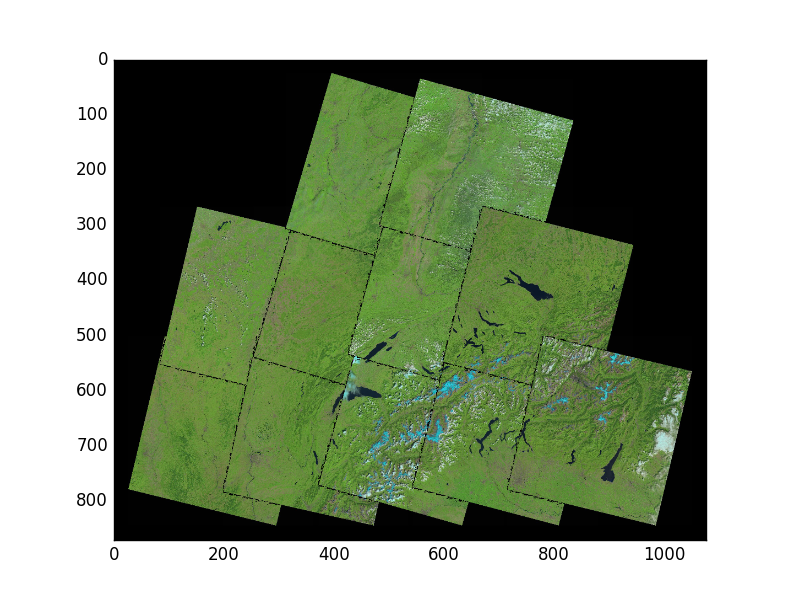
\includegraphics[scale=0.20]{images/Switzerland/covering-selection.png}
  \end{overlayarea}
  \begin{overlayarea}{\linewidth}{1cm}
    \centering
    \tiny Switzerland datasets georeferenced in $UTM$ system\par
  \end{overlayarea}
  \end{column}
  \begin{column}{0.33\textwidth}
   \begin{overlayarea}{\linewidth}{3cm}
    \centering\vfill
    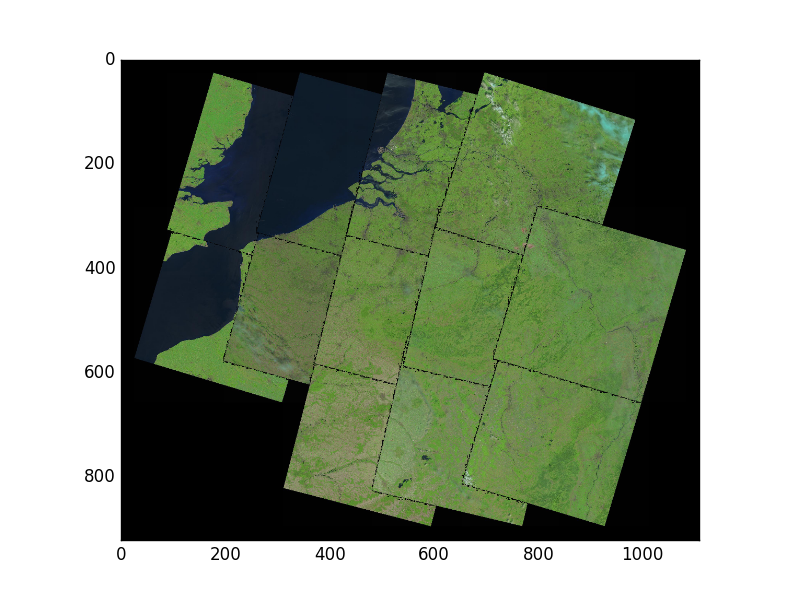
\includegraphics[scale=0.20]{images/Belgium/covering-selection.png}
  \end{overlayarea}
  \begin{overlayarea}{\linewidth}{1cm}
    \centering
    \tiny Belgium datasets georeferenced in $UTM$ system\par
  \end{overlayarea}
  \end{column}
  \begin{column}{0.33\textwidth}
  \begin{overlayarea}{\linewidth}{3cm}
    \centering\vfill
    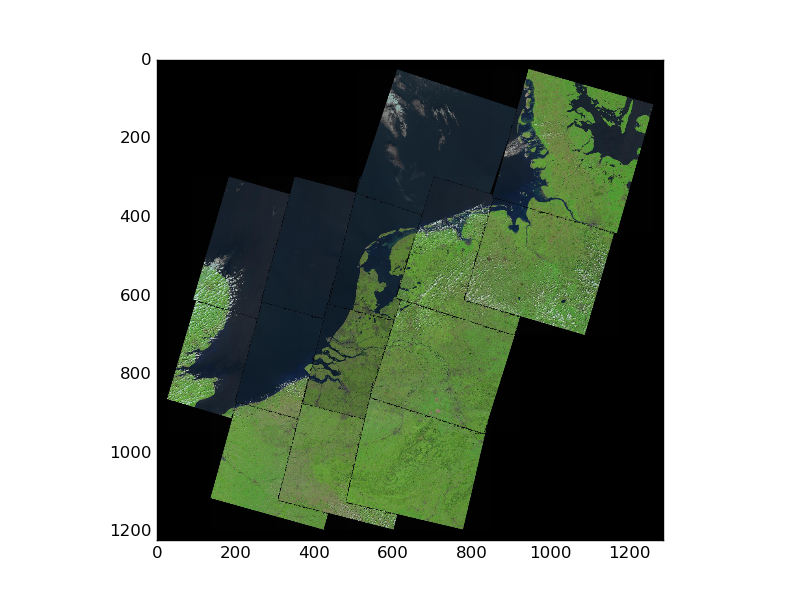
\includegraphics[scale=0.20]{images/Netherlands/covering-selection.png}
  \end{overlayarea}
  \begin{overlayarea}{\linewidth}{1cm}
    \centering
    \tiny Netherlands datasets georeferenced in $UTM$ system\par
  \end{overlayarea}
  \end{column}
 \end{columns}
}
\end{itemize}

\end{frame}

\subsection{K-Nearest Neighbors}

\begin{frame}
\begin{columns}
 \begin{column}{0.5\textwidth}
  \begin{overlayarea}{\linewidth}{4cm}
    \centering\vfill
    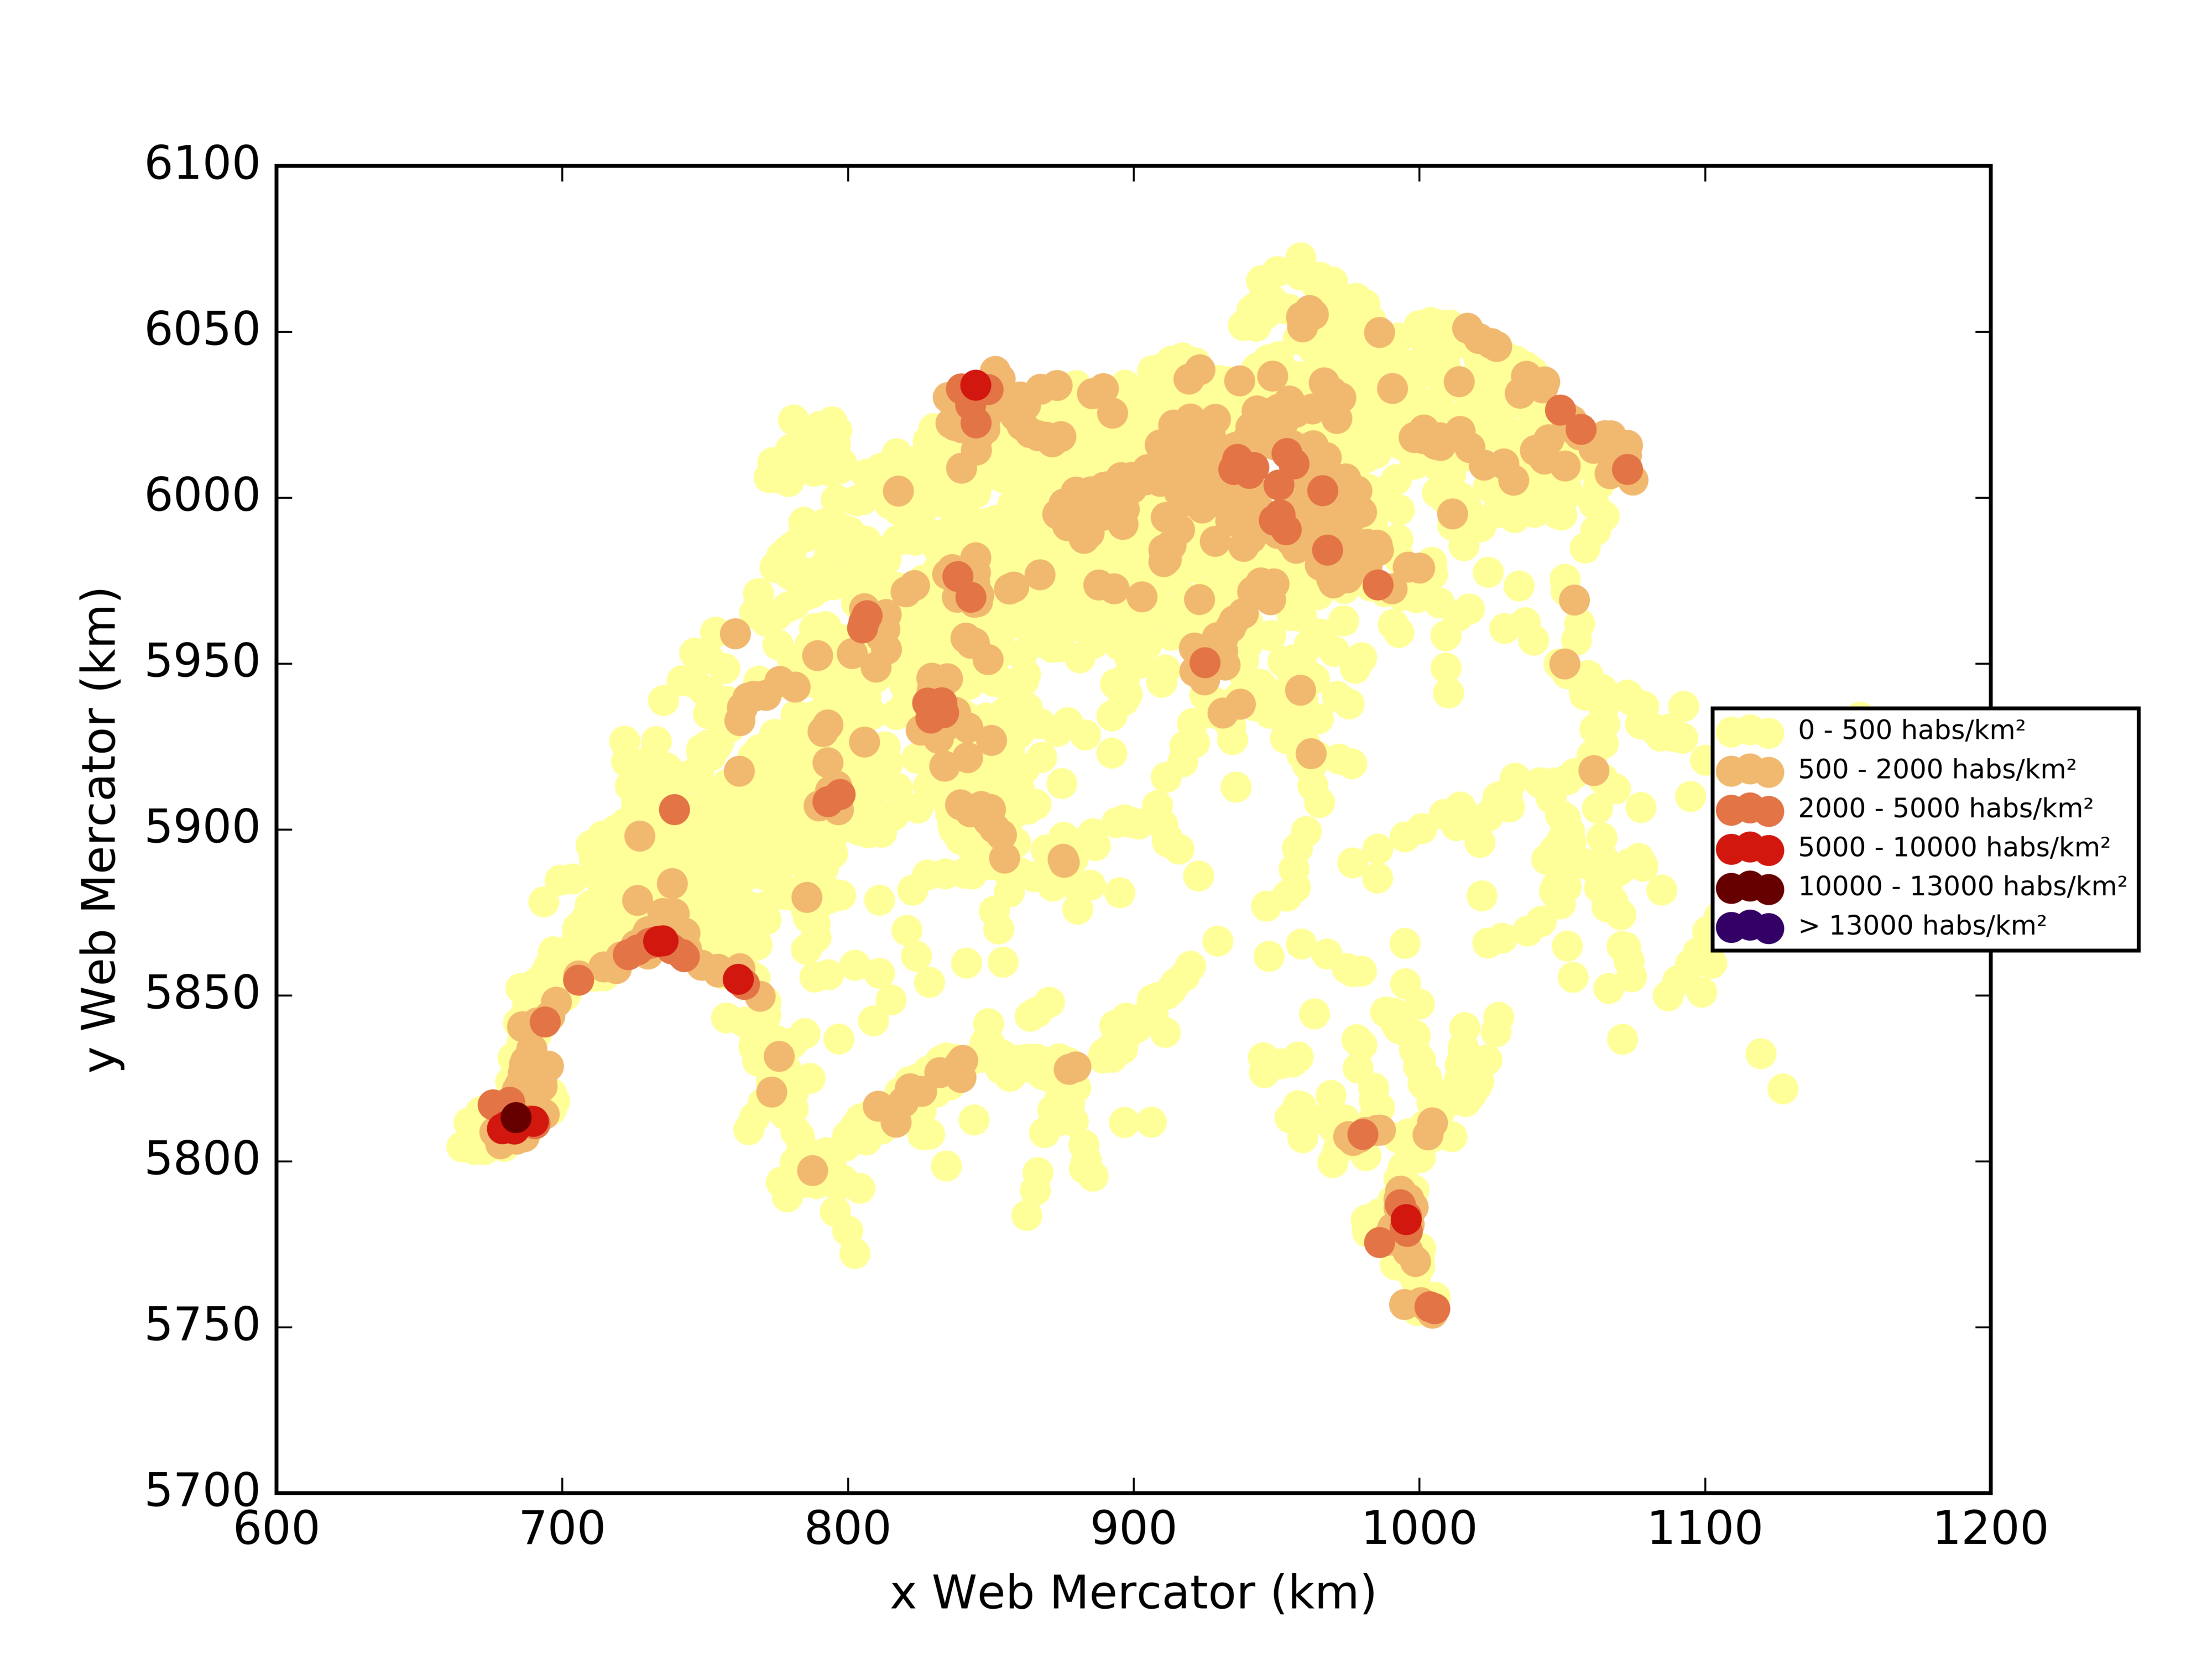
\includegraphics[scale=0.50]{images/Switzerland/density_ground_truth.png}
  \end{overlayarea}
  \begin{overlayarea}{\linewidth}{0.5cm}
    \centering
    \tiny Switzerland density category - ground truth\par
  \end{overlayarea}
 \end{column}
 \begin{column}{0.5\textwidth}
  \begin{overlayarea}{\linewidth}{4cm}
    \centering\vfill
    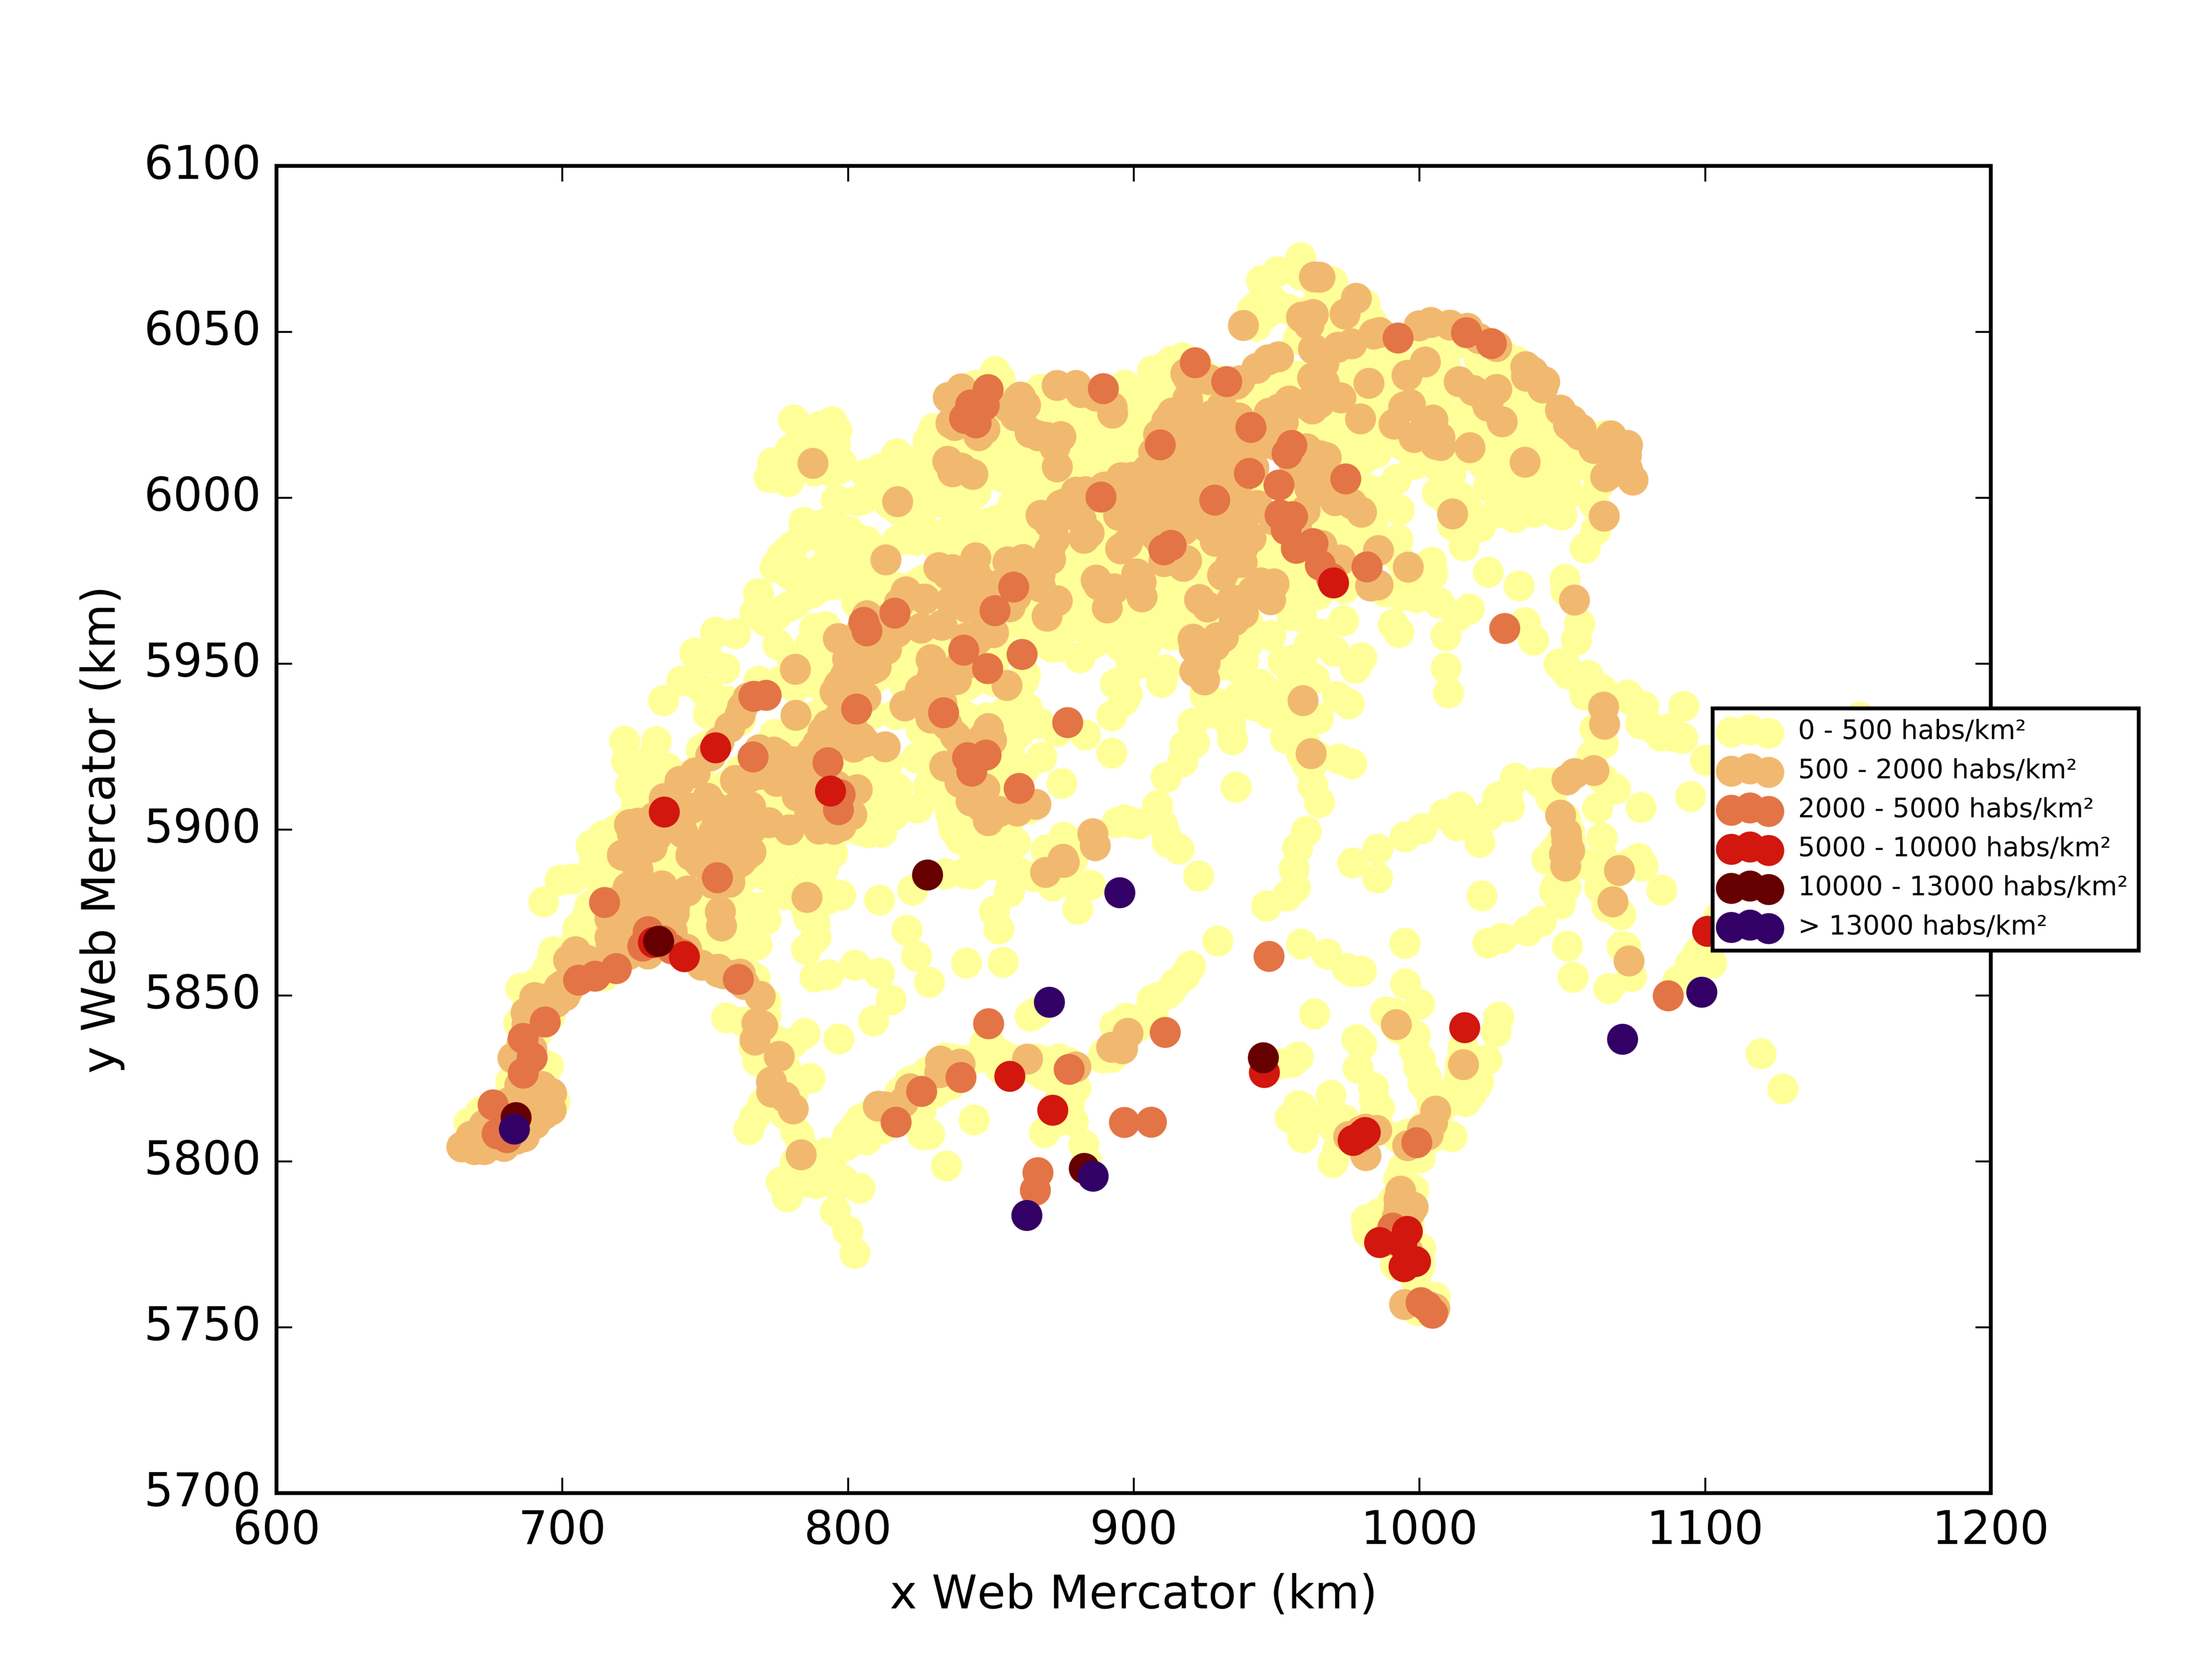
\includegraphics[scale=0.50]{images/Switzerland/knn/density_classification.png}
  \end{overlayarea}
  \begin{overlayarea}{\linewidth}{0.5cm}
    \centering
    \tiny Switzerland density category - prediction\par
  \end{overlayarea}
 \end{column}
\end{columns}
\begin{columns}
 \begin{column}{0.5\textwidth}
 \begin{overlayarea}{\linewidth}{2cm}
  \begin{table}
  \begin{center}
  \begin{adjustbox}{max width=0.7\textwidth}
  {\tiny
  \begin{tabular}{|c|c|c|c|c|c|c|}
    \hline
    \multicolumn{7}{|c|}{{\tiny \begin{bf}Confusion matrix\end{bf}}} \\
    \hline
     & \textbf{1} & \textbf{2} & \textbf{3} & \textbf{4} & \textbf{5} & \textbf{6}\\
    \hline
    \textbf{1} & 32533 & 0 & 0 & 0 & 0 & 0\\
    \hline
    \textbf{2} & 0 & 1252 & 0 & 0 & 0 & 0\\
    \hline
    \textbf{3} & 0 & 0 & 288 & 0 & 0 & 0\\
    \hline
    \textbf{4} & 0 & 0 & 0 & 78 & 0 & 0\\
    \hline
    \textbf{5} & 0 & 0 & 0 & 0 & 15 & 0\\
    \hline
    \textbf{6} & 0 & 0 & 0 & 0 & 0 & 24\\
    \hline
  \end{tabular}
  }
  \end{adjustbox}
  \end{center}
  \end{table}
 \end{overlayarea}
 \end{column}
 \begin{column}{0.5\textwidth}
 \begin{overlayarea}{\linewidth}{2cm}
  \begin{table}
    \begin{center}
    \begin{adjustbox}{max width=0.4\textwidth}
    {\tiny 
    \begin{tabular}{|c|c|}
      \hline
      \multicolumn{2}{|c|}{\begin{bf}Mean score per class\end{bf}} \\
      \hline
      \textbf{category} & \textbf{mean score}\\
      \hline
      \textbf{1} & 100\% \\
      \hline
      \textbf{2} & 100\% \\
      \hline
      \textbf{3} & 100\% \\
      \hline
      \textbf{4} & 100\% \\
      \hline
      \textbf{5} & 100\% \\
      \hline
      \textbf{6} & 100\% \\
      \hline
      \textbf{mean} & 100\% \\
      \hline
    \end{tabular}
    }
    \end{adjustbox}
    \end{center}
  \end{table}
  \end{overlayarea}
\end{column}
\end{columns}
\end{frame}

\begin{frame}
\begin{columns}
 \begin{column}{0.5\textwidth}
  \begin{overlayarea}{\linewidth}{4cm}
    \centering\vfill
    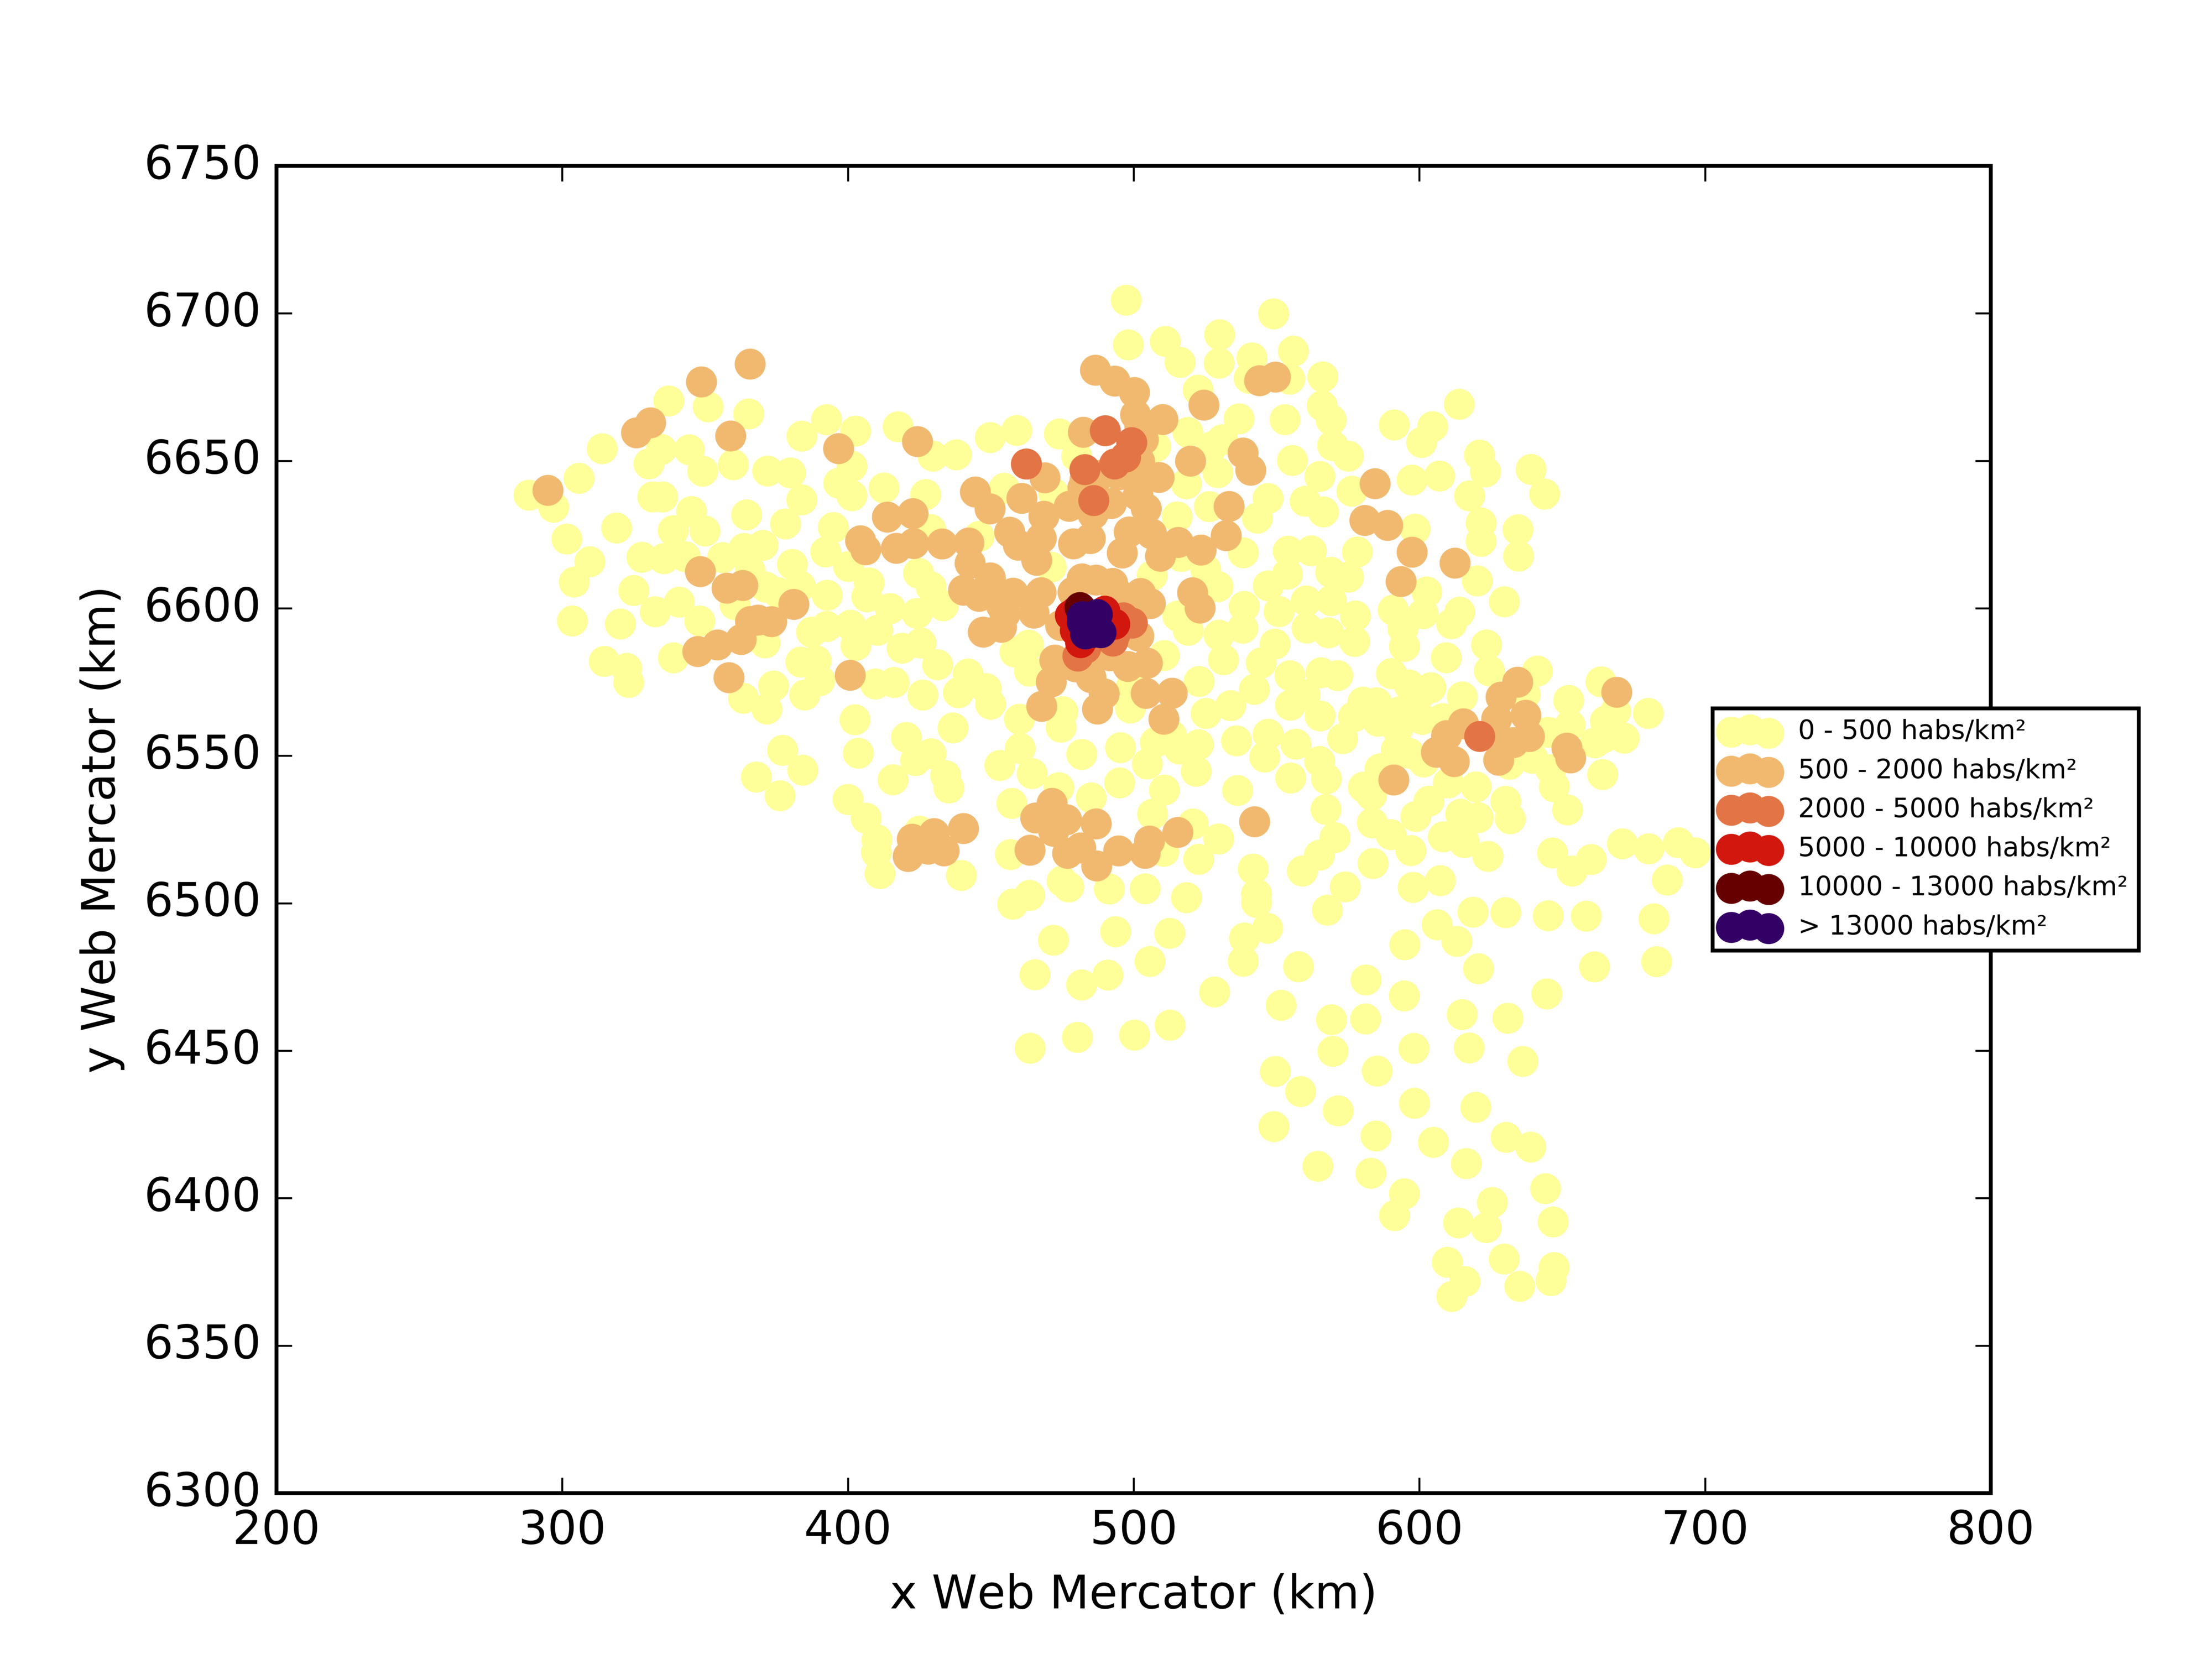
\includegraphics[scale=0.50]{images/Belgium/density_ground_truth.png}
  \end{overlayarea}
  \begin{overlayarea}{\linewidth}{0.5cm}
    \centering
    \tiny Switzerland density category - ground truth\par
  \end{overlayarea}
 \end{column}
 \begin{column}{0.5\textwidth}
  \begin{overlayarea}{\linewidth}{4cm}
    \centering\vfill
    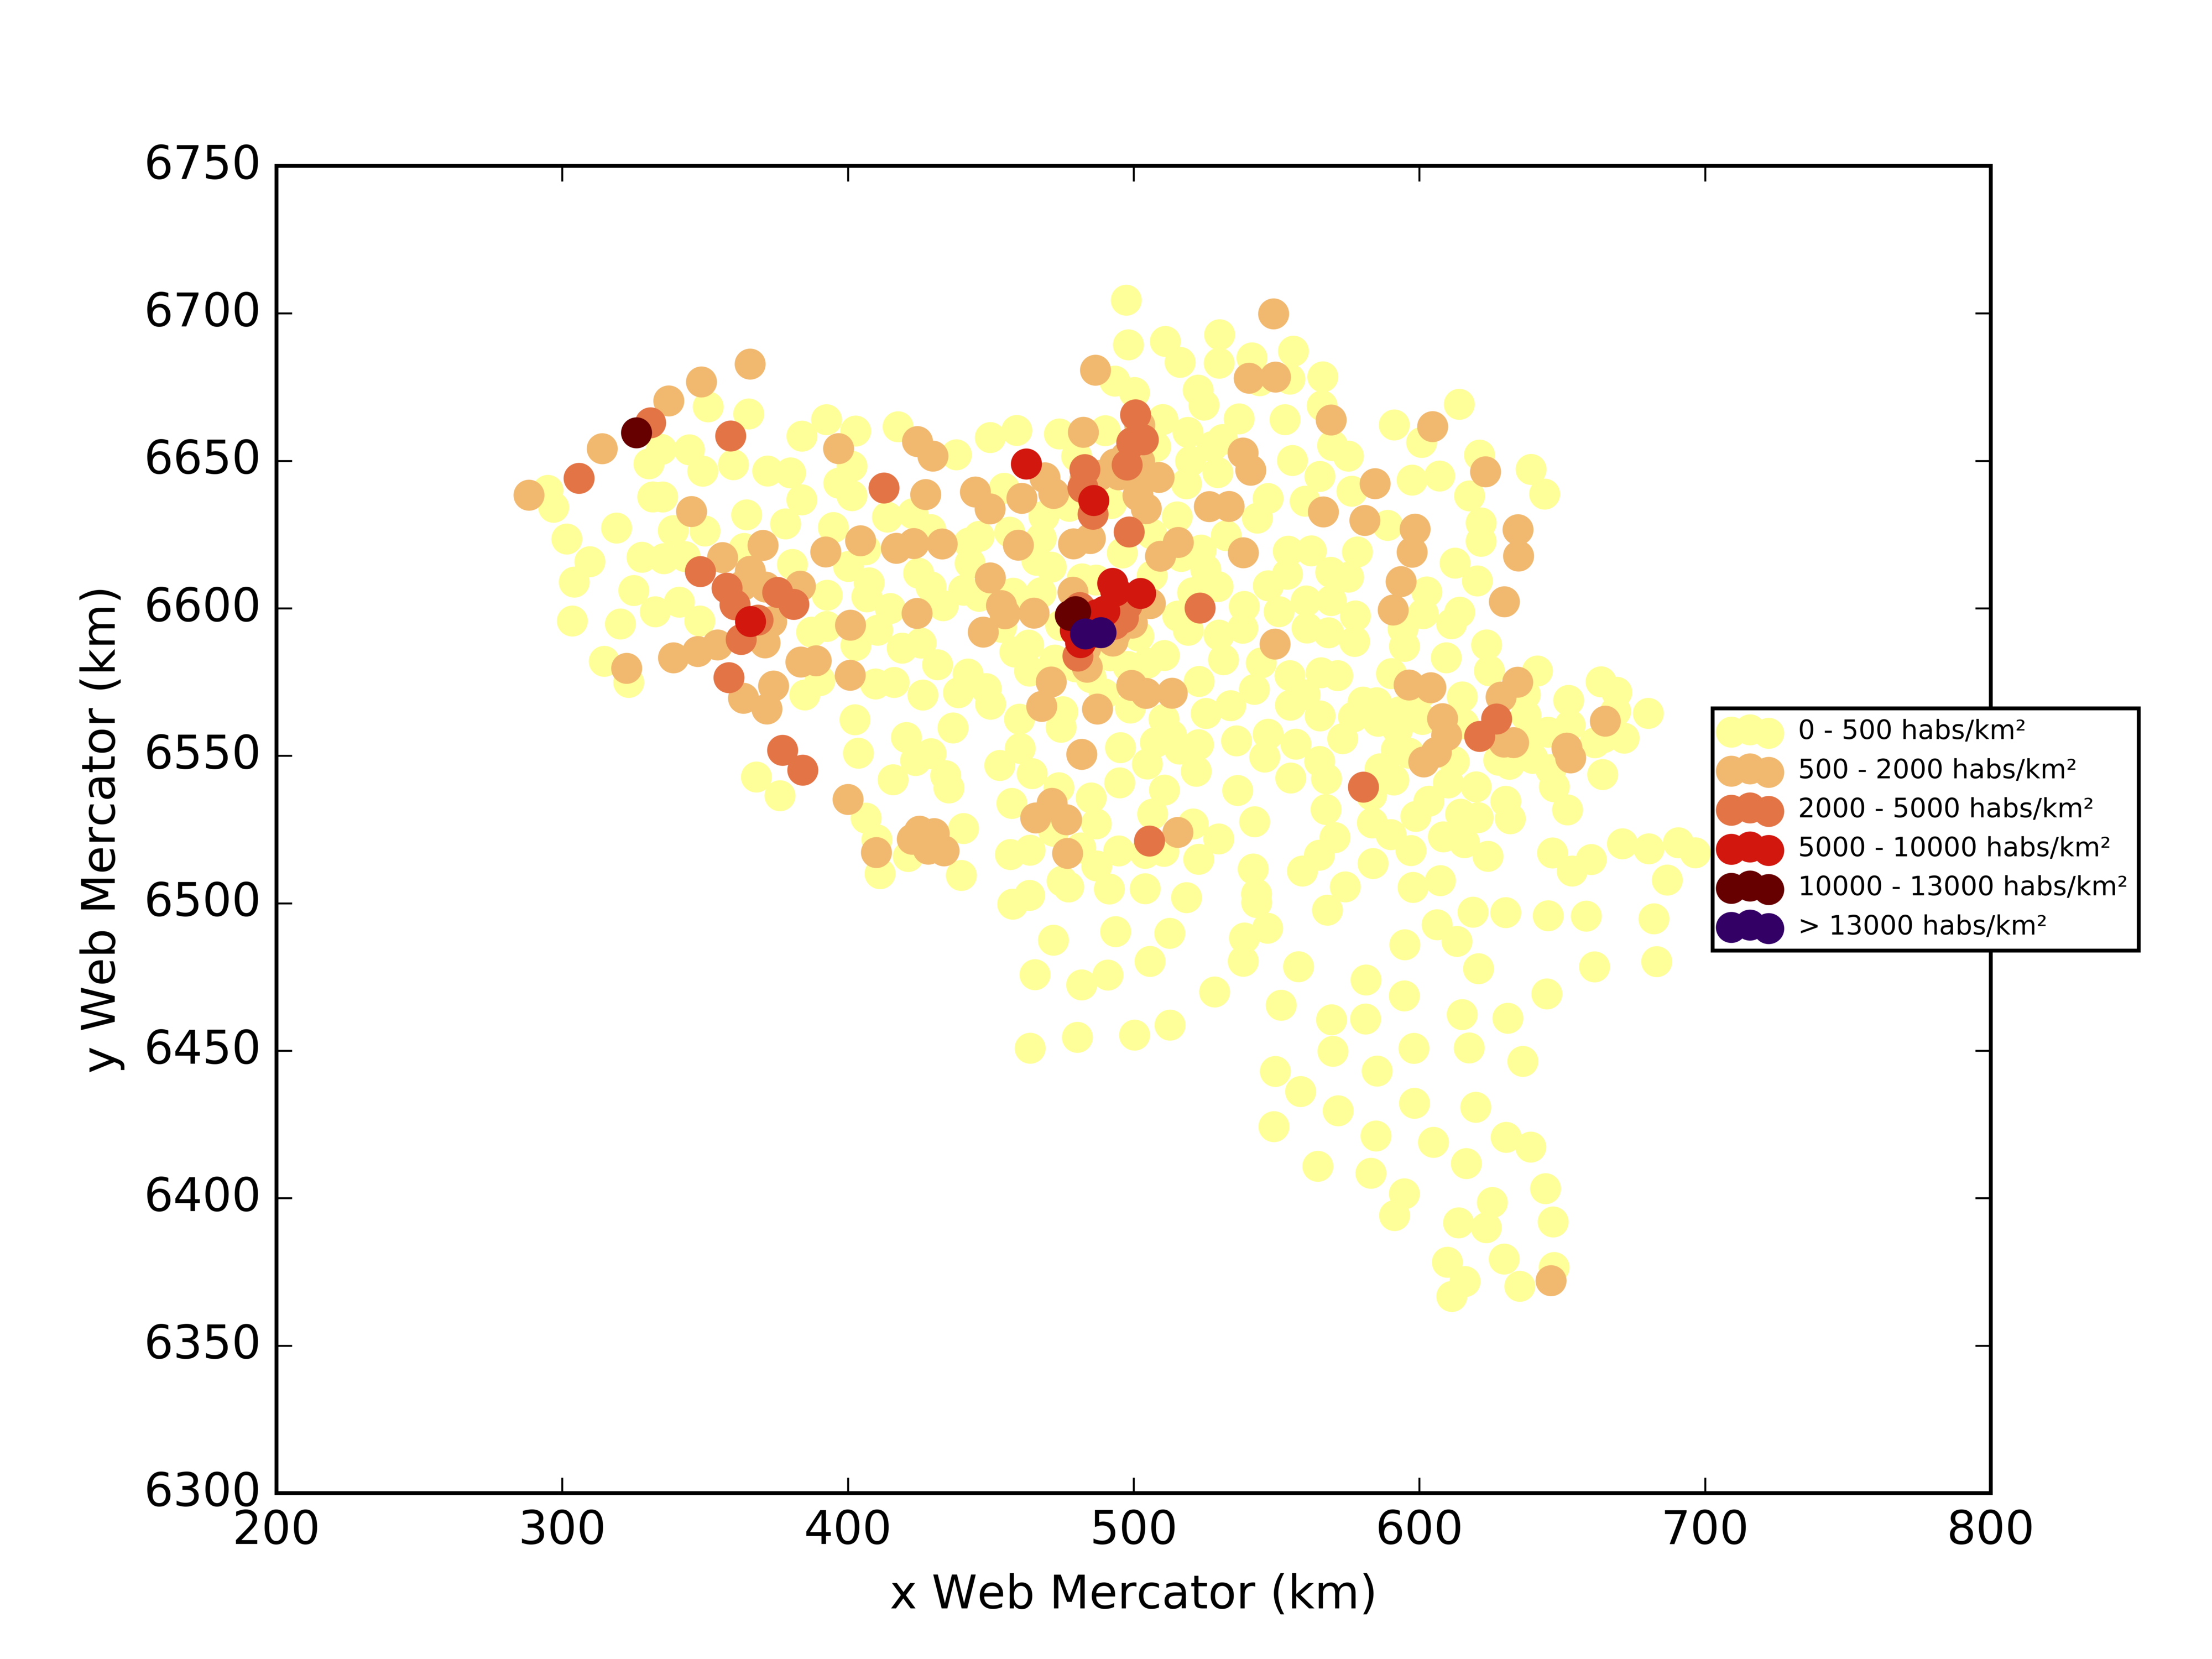
\includegraphics[scale=0.50]{images/Belgium/knn/density_classification.png}
  \end{overlayarea}
  \begin{overlayarea}{\linewidth}{0.5cm}
    \centering
    \tiny Switzerland density category - prediction\par
  \end{overlayarea}
 \end{column}
\end{columns}
\begin{columns}
 \begin{column}{0.5\textwidth}
 \begin{overlayarea}{\linewidth}{2cm}
  \begin{table}
  \begin{center}
  \begin{adjustbox}{max width=0.7\textwidth}
  {\tiny
  \begin{tabular}{|c|c|c|c|c|c|c|}
    \hline
    \multicolumn{7}{|c|}{{\tiny \begin{bf}Confusion matrix\end{bf}}} \\
    \hline
     & \textbf{1} & \textbf{2} & \textbf{3} & \textbf{4} & \textbf{5} & \textbf{6}\\
    \hline
    \textbf{1} & 32533 & 0 & 0 & 0 & 0 & 0\\
    \hline
    \textbf{2} & 0 & 1252 & 0 & 0 & 0 & 0\\
    \hline
    \textbf{3} & 0 & 0 & 288 & 0 & 0 & 0\\
    \hline
    \textbf{4} & 0 & 0 & 0 & 78 & 0 & 0\\
    \hline
    \textbf{5} & 0 & 0 & 0 & 0 & 15 & 0\\
    \hline
    \textbf{6} & 0 & 0 & 0 & 0 & 0 & 24\\
    \hline
  \end{tabular}
  }
  \end{adjustbox}
  \end{center}
  \end{table}
 \end{overlayarea}
 \end{column}
 \begin{column}{0.5\textwidth}
 \begin{overlayarea}{\linewidth}{2cm}
  \begin{table}
    \begin{center}
    \begin{adjustbox}{max width=0.4\textwidth}
    {\tiny 
    \begin{tabular}{|c|c|}
      \hline
      \multicolumn{2}{|c|}{\begin{bf}Mean score per class\end{bf}} \\
      \hline
      \textbf{category} & \textbf{mean score}\\
      \hline
      \textbf{1} & 100\% \\
      \hline
      \textbf{2} & 100\% \\
      \hline
      \textbf{3} & 100\% \\
      \hline
      \textbf{4} & 100\% \\
      \hline
      \textbf{5} & 100\% \\
      \hline
      \textbf{6} & 100\% \\
      \hline
      \textbf{mean} & 100\% \\
      \hline
    \end{tabular}
    }
    \end{adjustbox}
    \end{center}
  \end{table}
  \end{overlayarea}
\end{column}
\end{columns}
\end{frame}

\begin{frame}
\begin{columns}
 \begin{column}{0.5\textwidth}
  \begin{overlayarea}{\linewidth}{4cm}
    \centering\vfill
    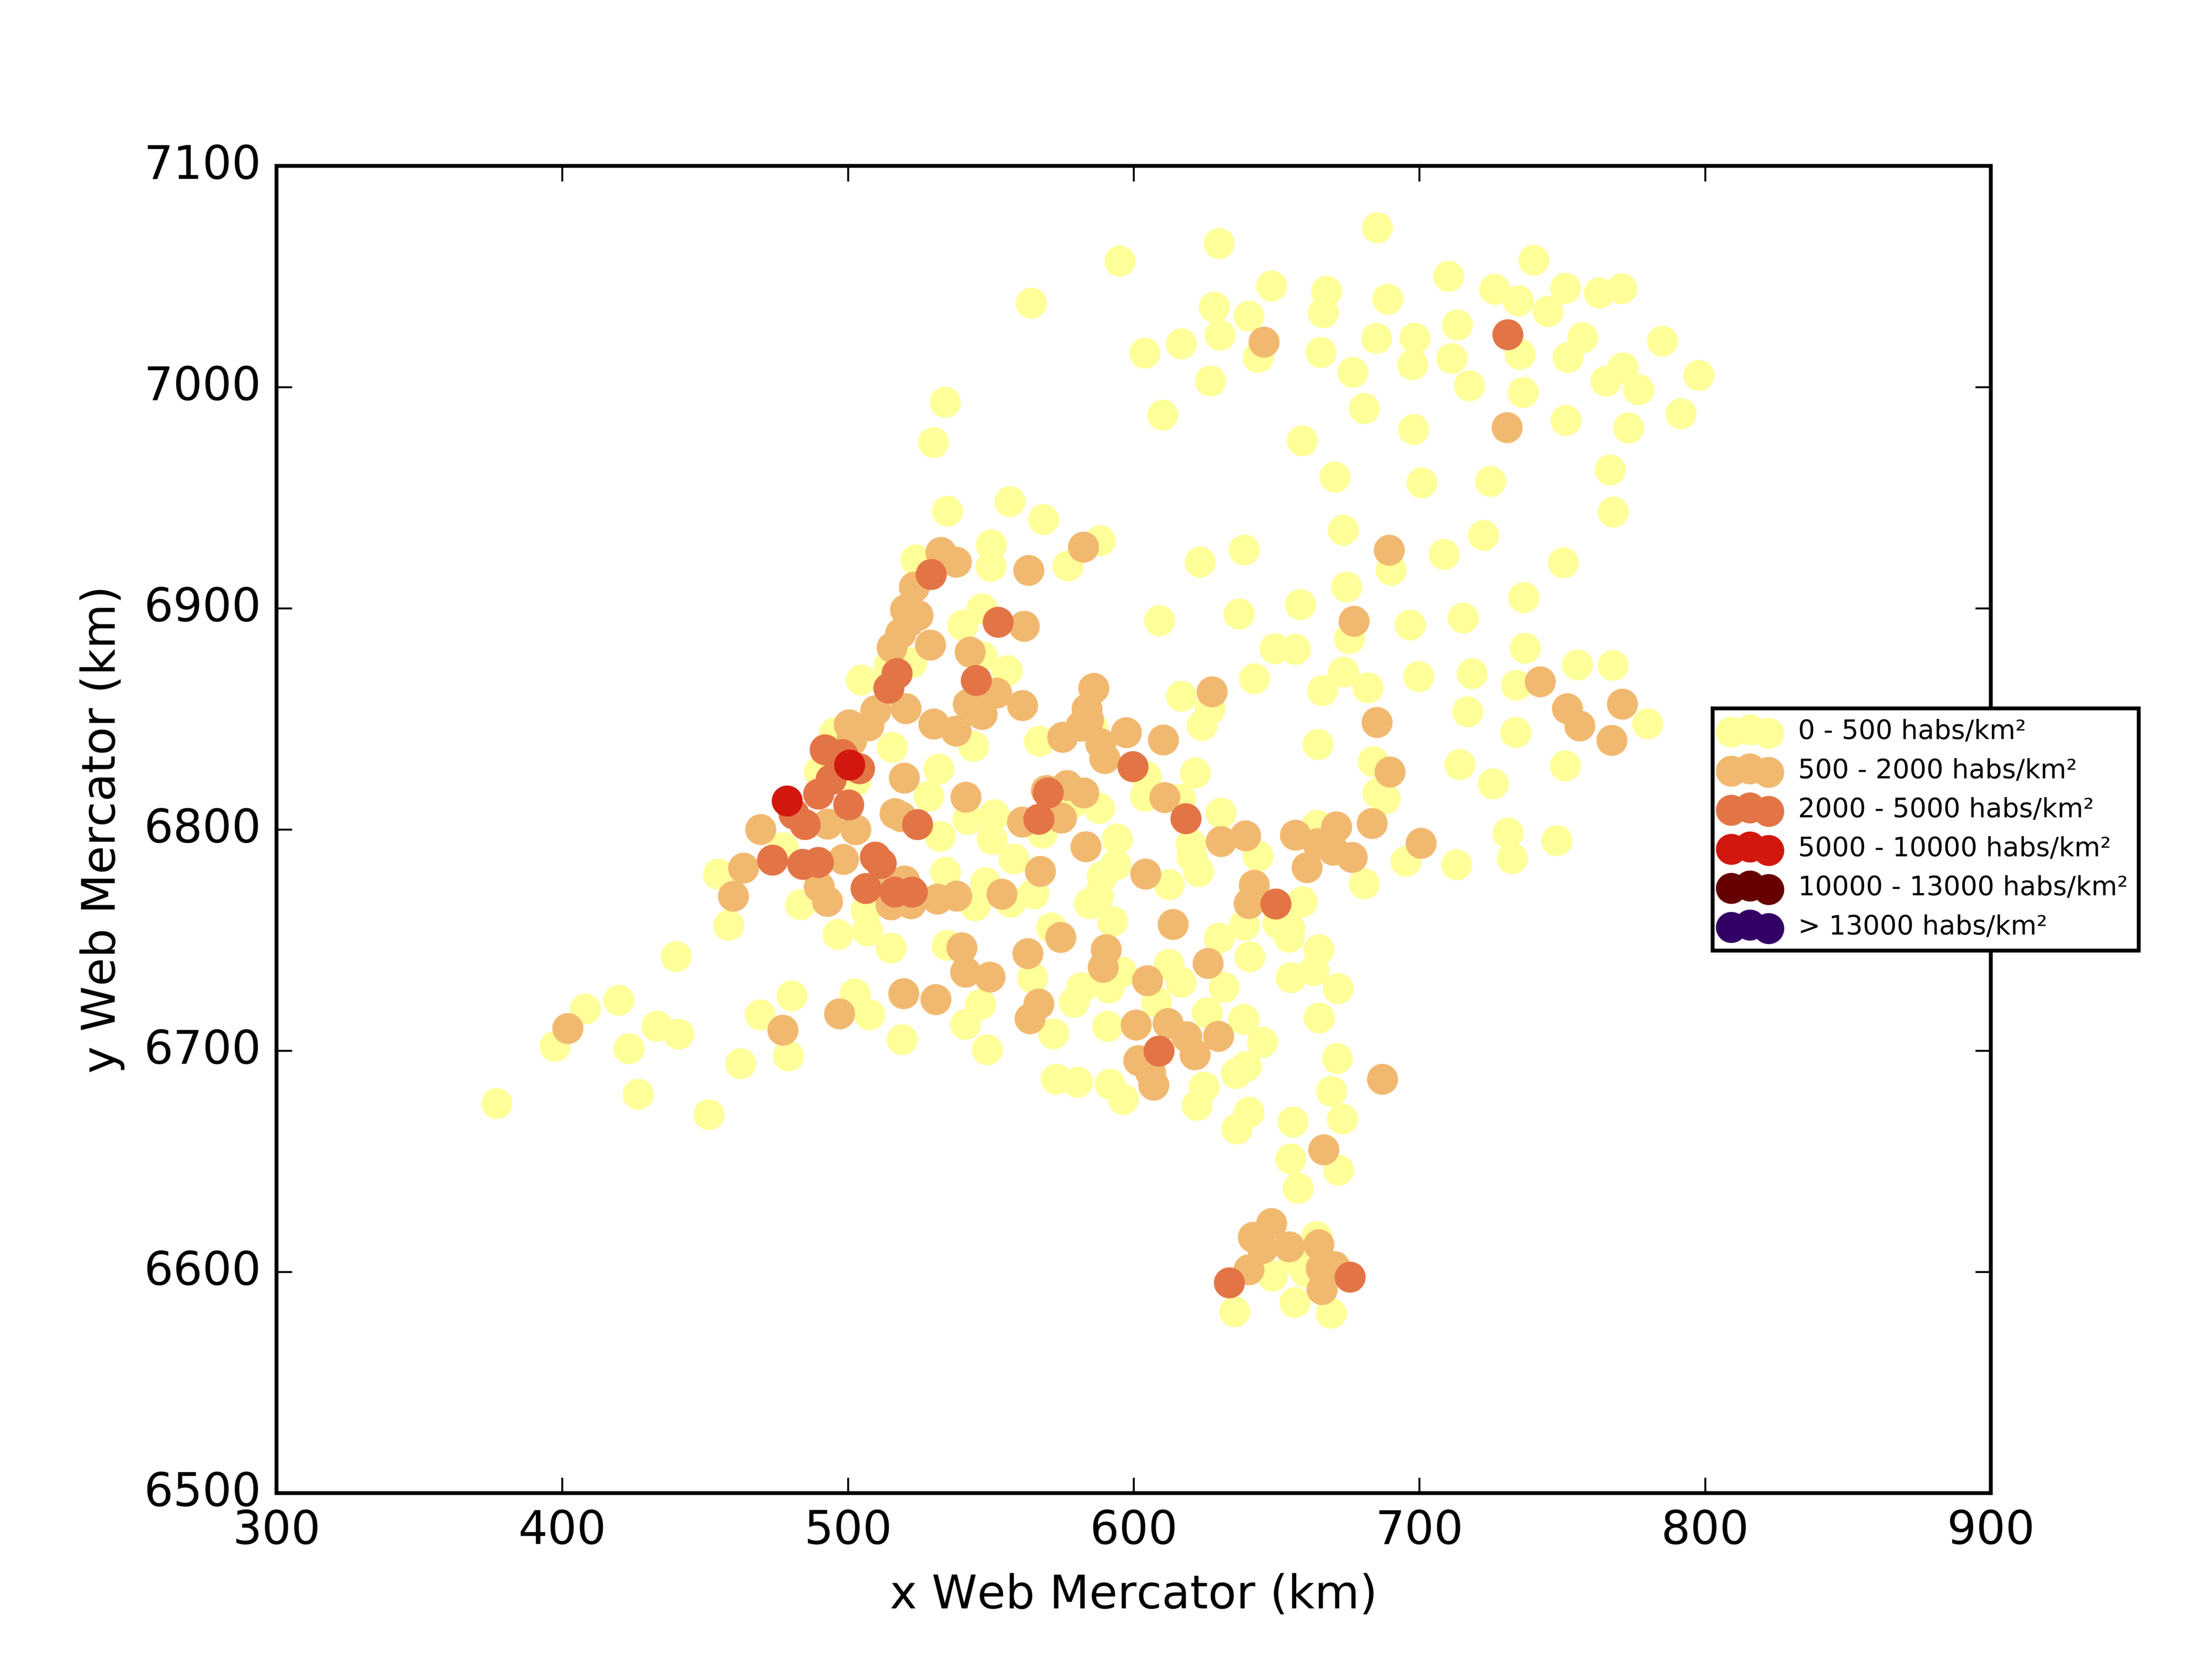
\includegraphics[scale=0.50]{images/Netherlands/density_ground_truth.png}
  \end{overlayarea}
  \begin{overlayarea}{\linewidth}{0.5cm}
    \centering
    \tiny Switzerland density category - ground truth\par
  \end{overlayarea}
 \end{column}
 \begin{column}{0.5\textwidth}
  \begin{overlayarea}{\linewidth}{4cm}
    \centering\vfill
    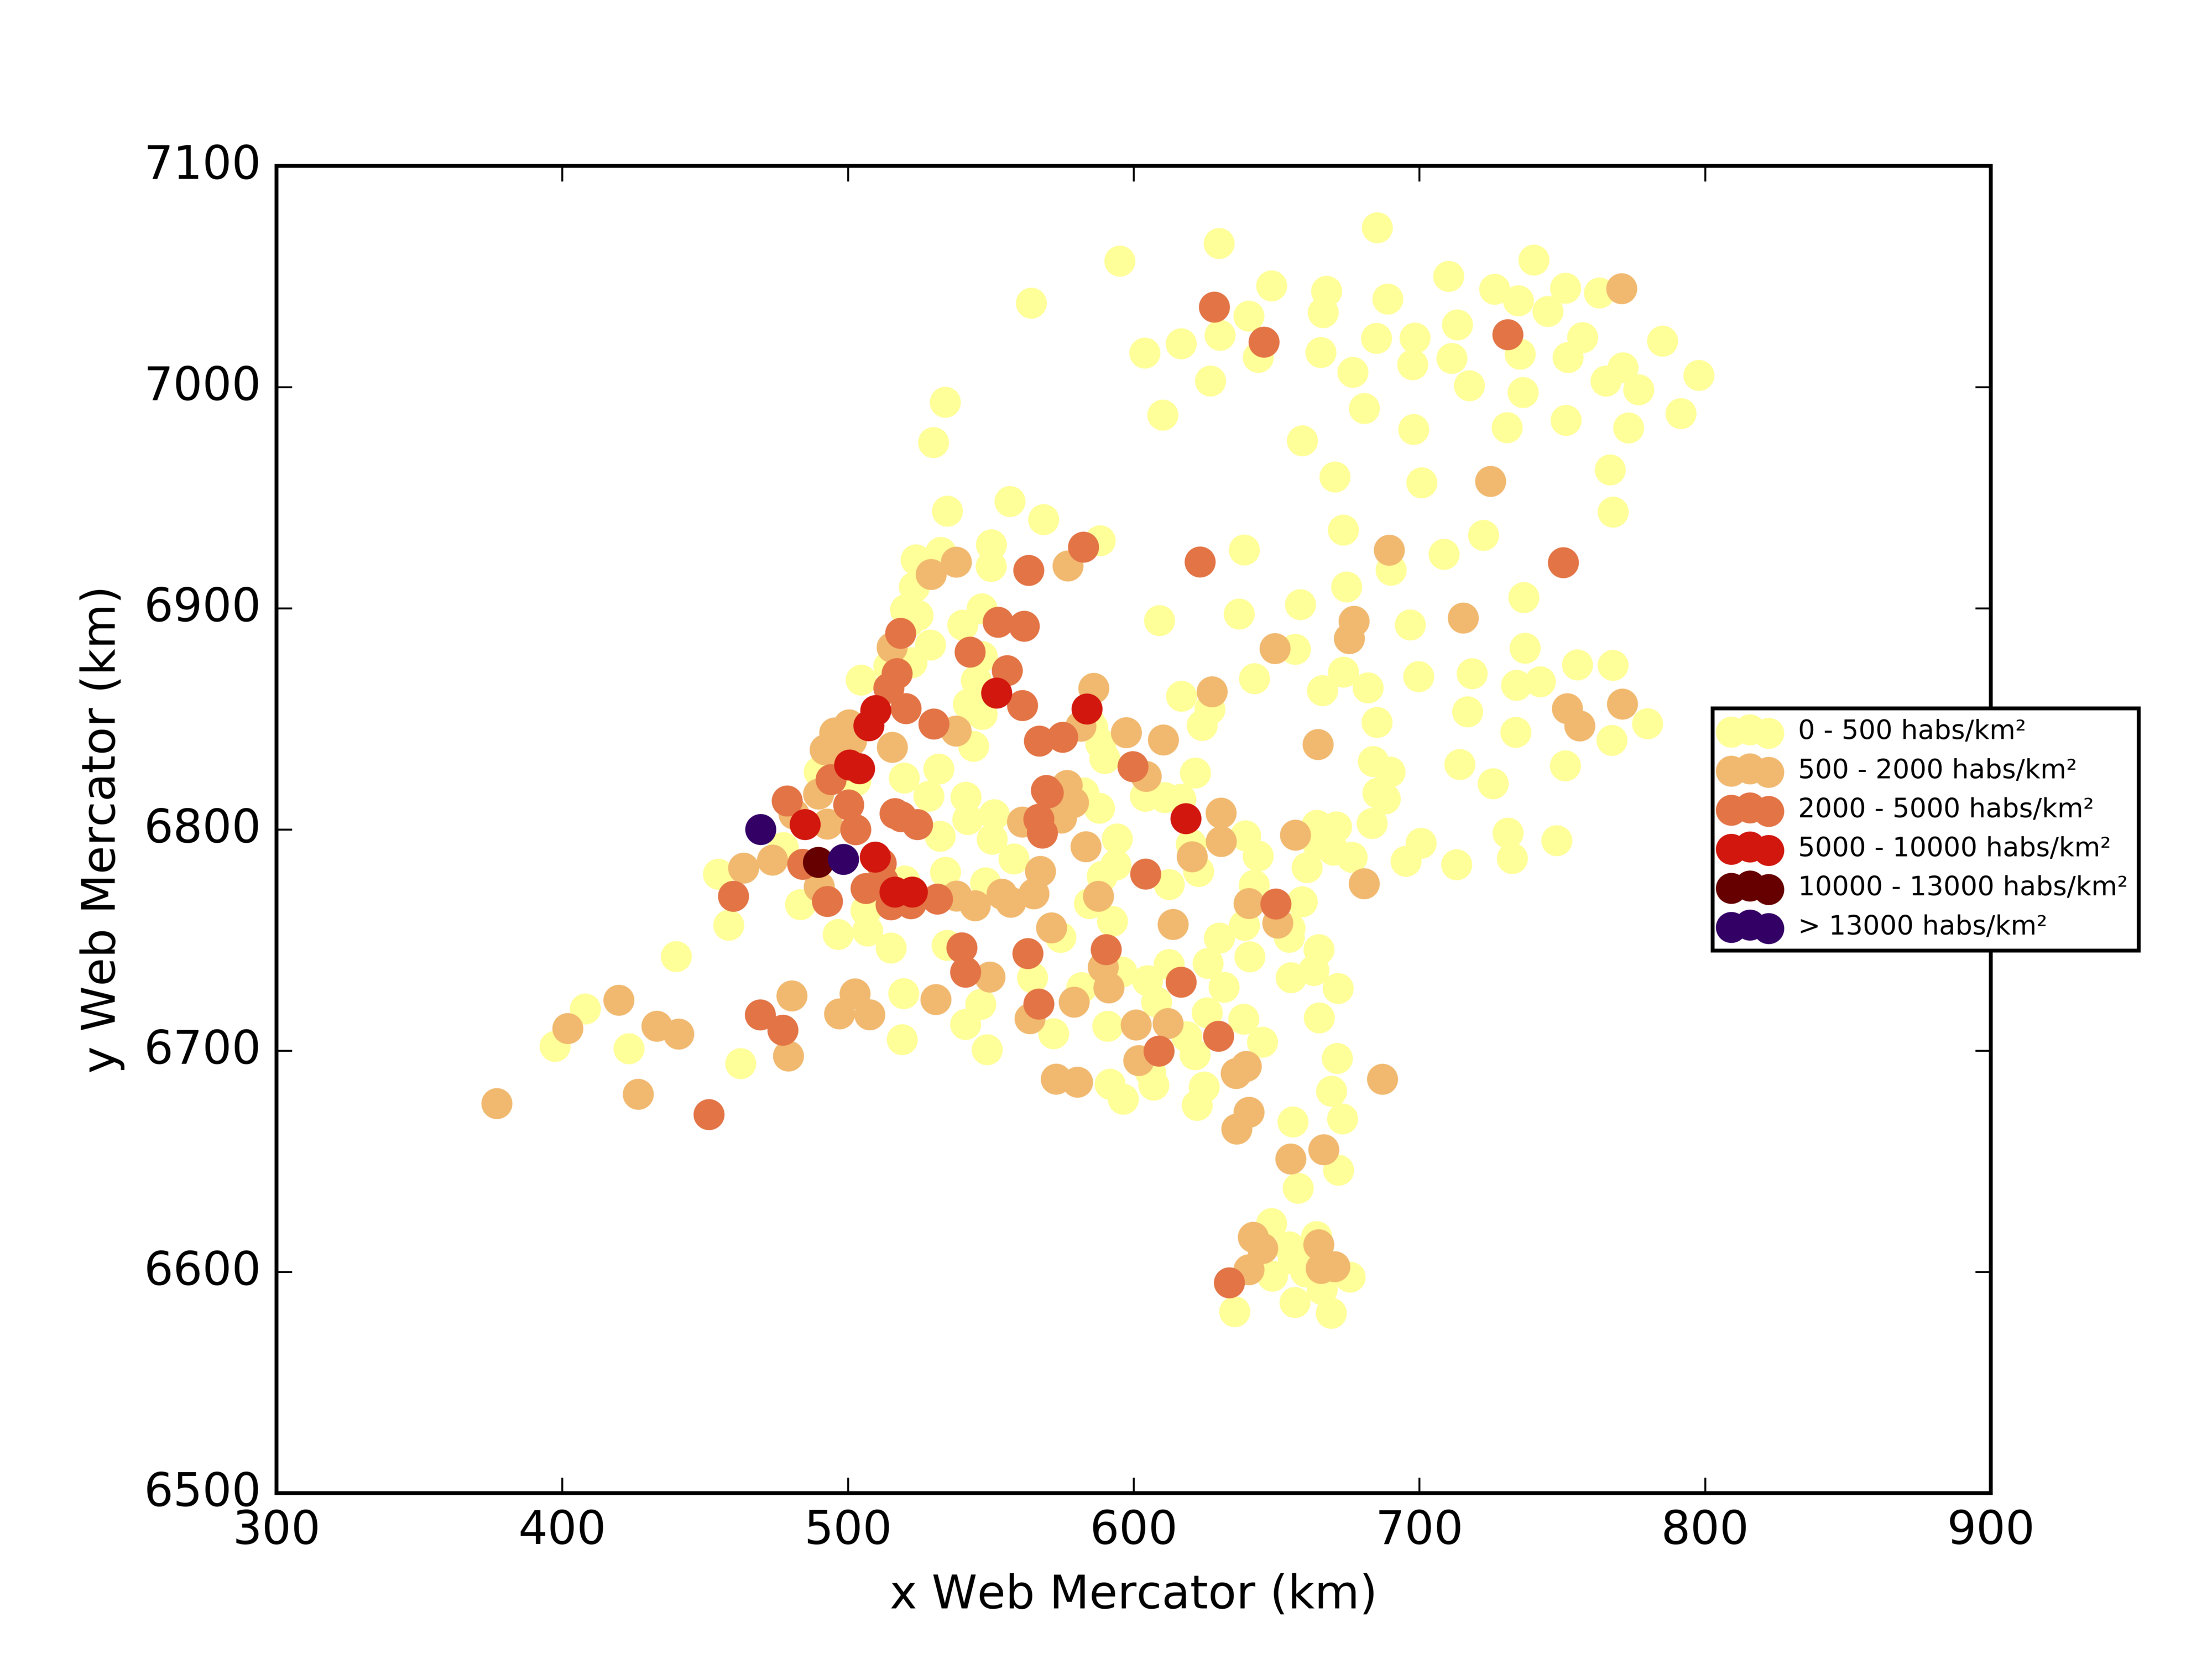
\includegraphics[scale=0.50]{images/Netherlands/knn/density_classification.png}
  \end{overlayarea}
  \begin{overlayarea}{\linewidth}{0.5cm}
    \centering
    \tiny Switzerland density category - prediction\par
  \end{overlayarea}
 \end{column}
\end{columns}
\begin{columns}
 \begin{column}{0.5\textwidth}
 \begin{overlayarea}{\linewidth}{2cm}
  \begin{table}
  \begin{center}
  \begin{adjustbox}{max width=0.7\textwidth}
  {\tiny
  \begin{tabular}{|c|c|c|c|c|c|c|}
    \hline
    \multicolumn{7}{|c|}{{\tiny \begin{bf}Confusion matrix\end{bf}}} \\
    \hline
     & \textbf{1} & \textbf{2} & \textbf{3} & \textbf{4} & \textbf{5} & \textbf{6}\\
    \hline
    \textbf{1} & 32533 & 0 & 0 & 0 & 0 & 0\\
    \hline
    \textbf{2} & 0 & 1252 & 0 & 0 & 0 & 0\\
    \hline
    \textbf{3} & 0 & 0 & 288 & 0 & 0 & 0\\
    \hline
    \textbf{4} & 0 & 0 & 0 & 78 & 0 & 0\\
    \hline
    \textbf{5} & 0 & 0 & 0 & 0 & 15 & 0\\
    \hline
    \textbf{6} & 0 & 0 & 0 & 0 & 0 & 24\\
    \hline
  \end{tabular}
  }
  \end{adjustbox}
  \end{center}
  \end{table}
 \end{overlayarea}
 \end{column}
 \begin{column}{0.5\textwidth}
 \begin{overlayarea}{\linewidth}{2cm}
  \begin{table}
    \begin{center}
    \begin{adjustbox}{max width=0.4\textwidth}
    {\tiny 
    \begin{tabular}{|c|c|}
      \hline
      \multicolumn{2}{|c|}{\begin{bf}Mean score per class\end{bf}} \\
      \hline
      \textbf{category} & \textbf{mean score}\\
      \hline
      \textbf{1} & 100\% \\
      \hline
      \textbf{2} & 100\% \\
      \hline
      \textbf{3} & 100\% \\
      \hline
      \textbf{4} & 100\% \\
      \hline
      \textbf{5} & 100\% \\
      \hline
      \textbf{6} & 100\% \\
      \hline
      \textbf{mean} & 100\% \\
      \hline
    \end{tabular}
    }
    \end{adjustbox}
    \end{center}
  \end{table}
  \end{overlayarea}
\end{column}
\end{columns}
\end{frame}

\subsection{Neural Network}

\begin{frame}
\begin{columns}
 \begin{column}{0.5\textwidth}
  \begin{overlayarea}{\linewidth}{4cm}
    \centering\vfill
    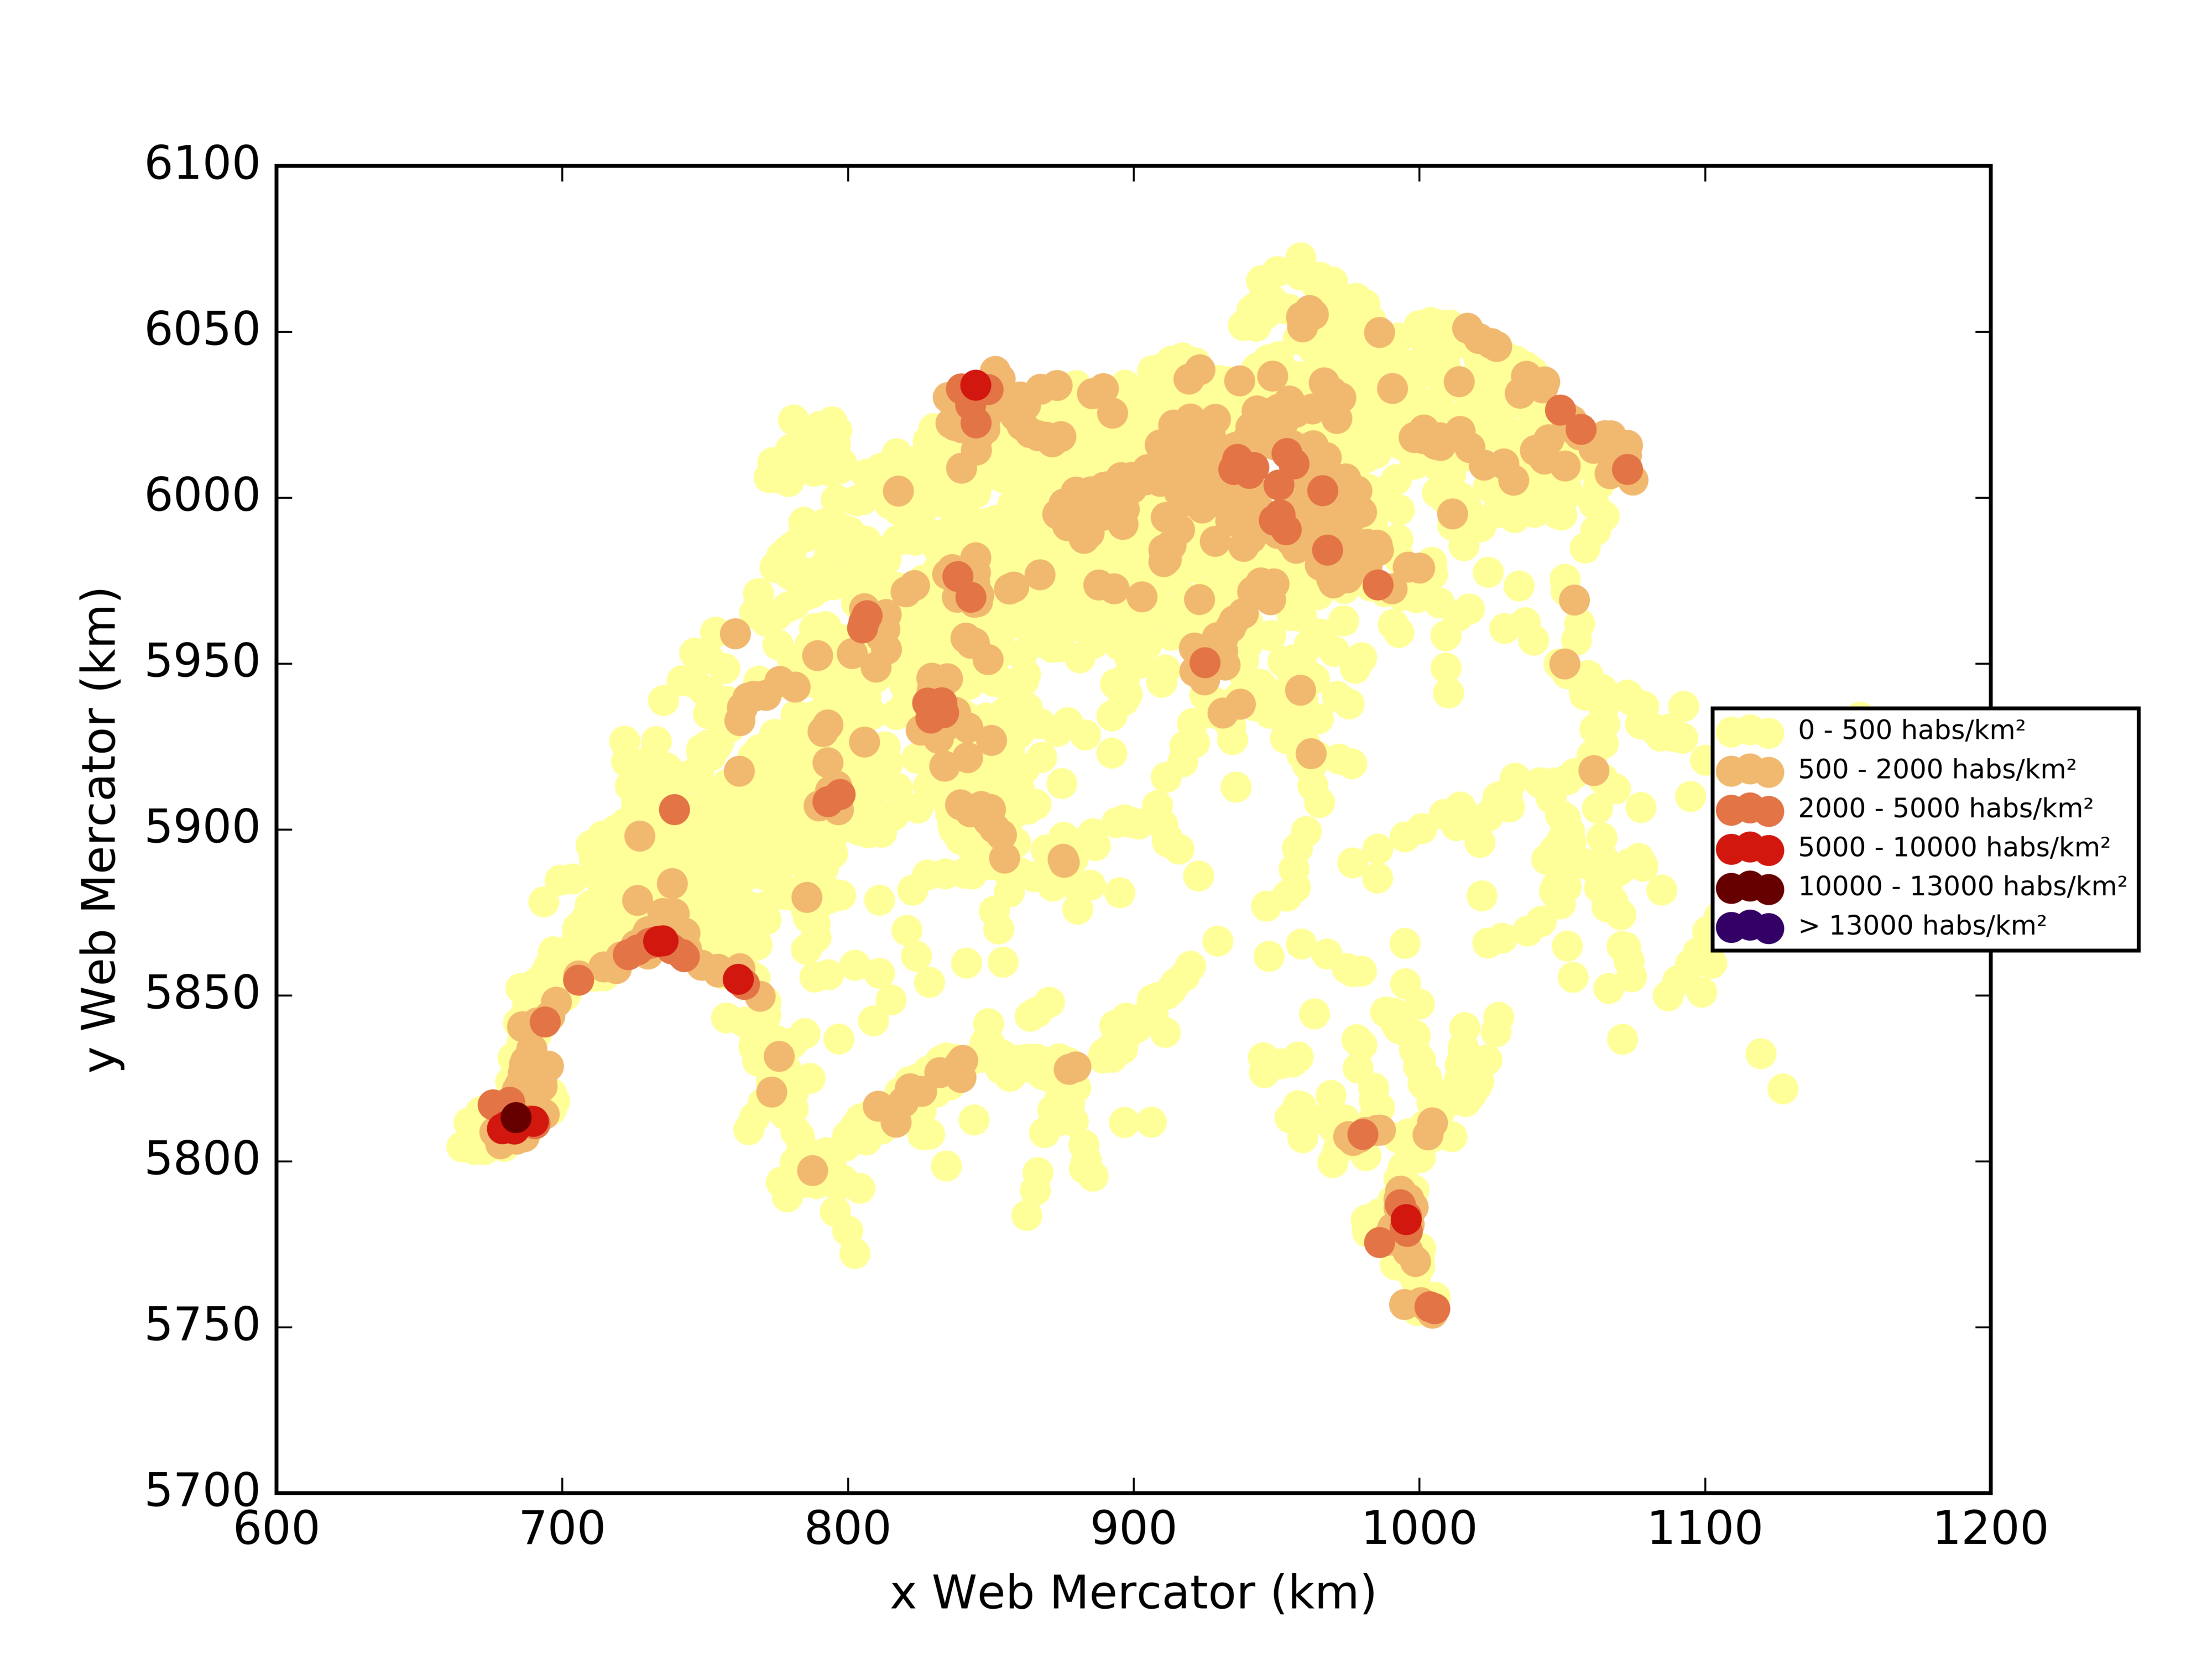
\includegraphics[scale=0.50]{images/Switzerland/density_ground_truth.png}
  \end{overlayarea}
  \begin{overlayarea}{\linewidth}{0.5cm}
    \centering
    \tiny Switzerland density category - ground truth\par
  \end{overlayarea}
 \end{column}
 \begin{column}{0.5\textwidth}
  \begin{overlayarea}{\linewidth}{4cm}
    \centering\vfill
    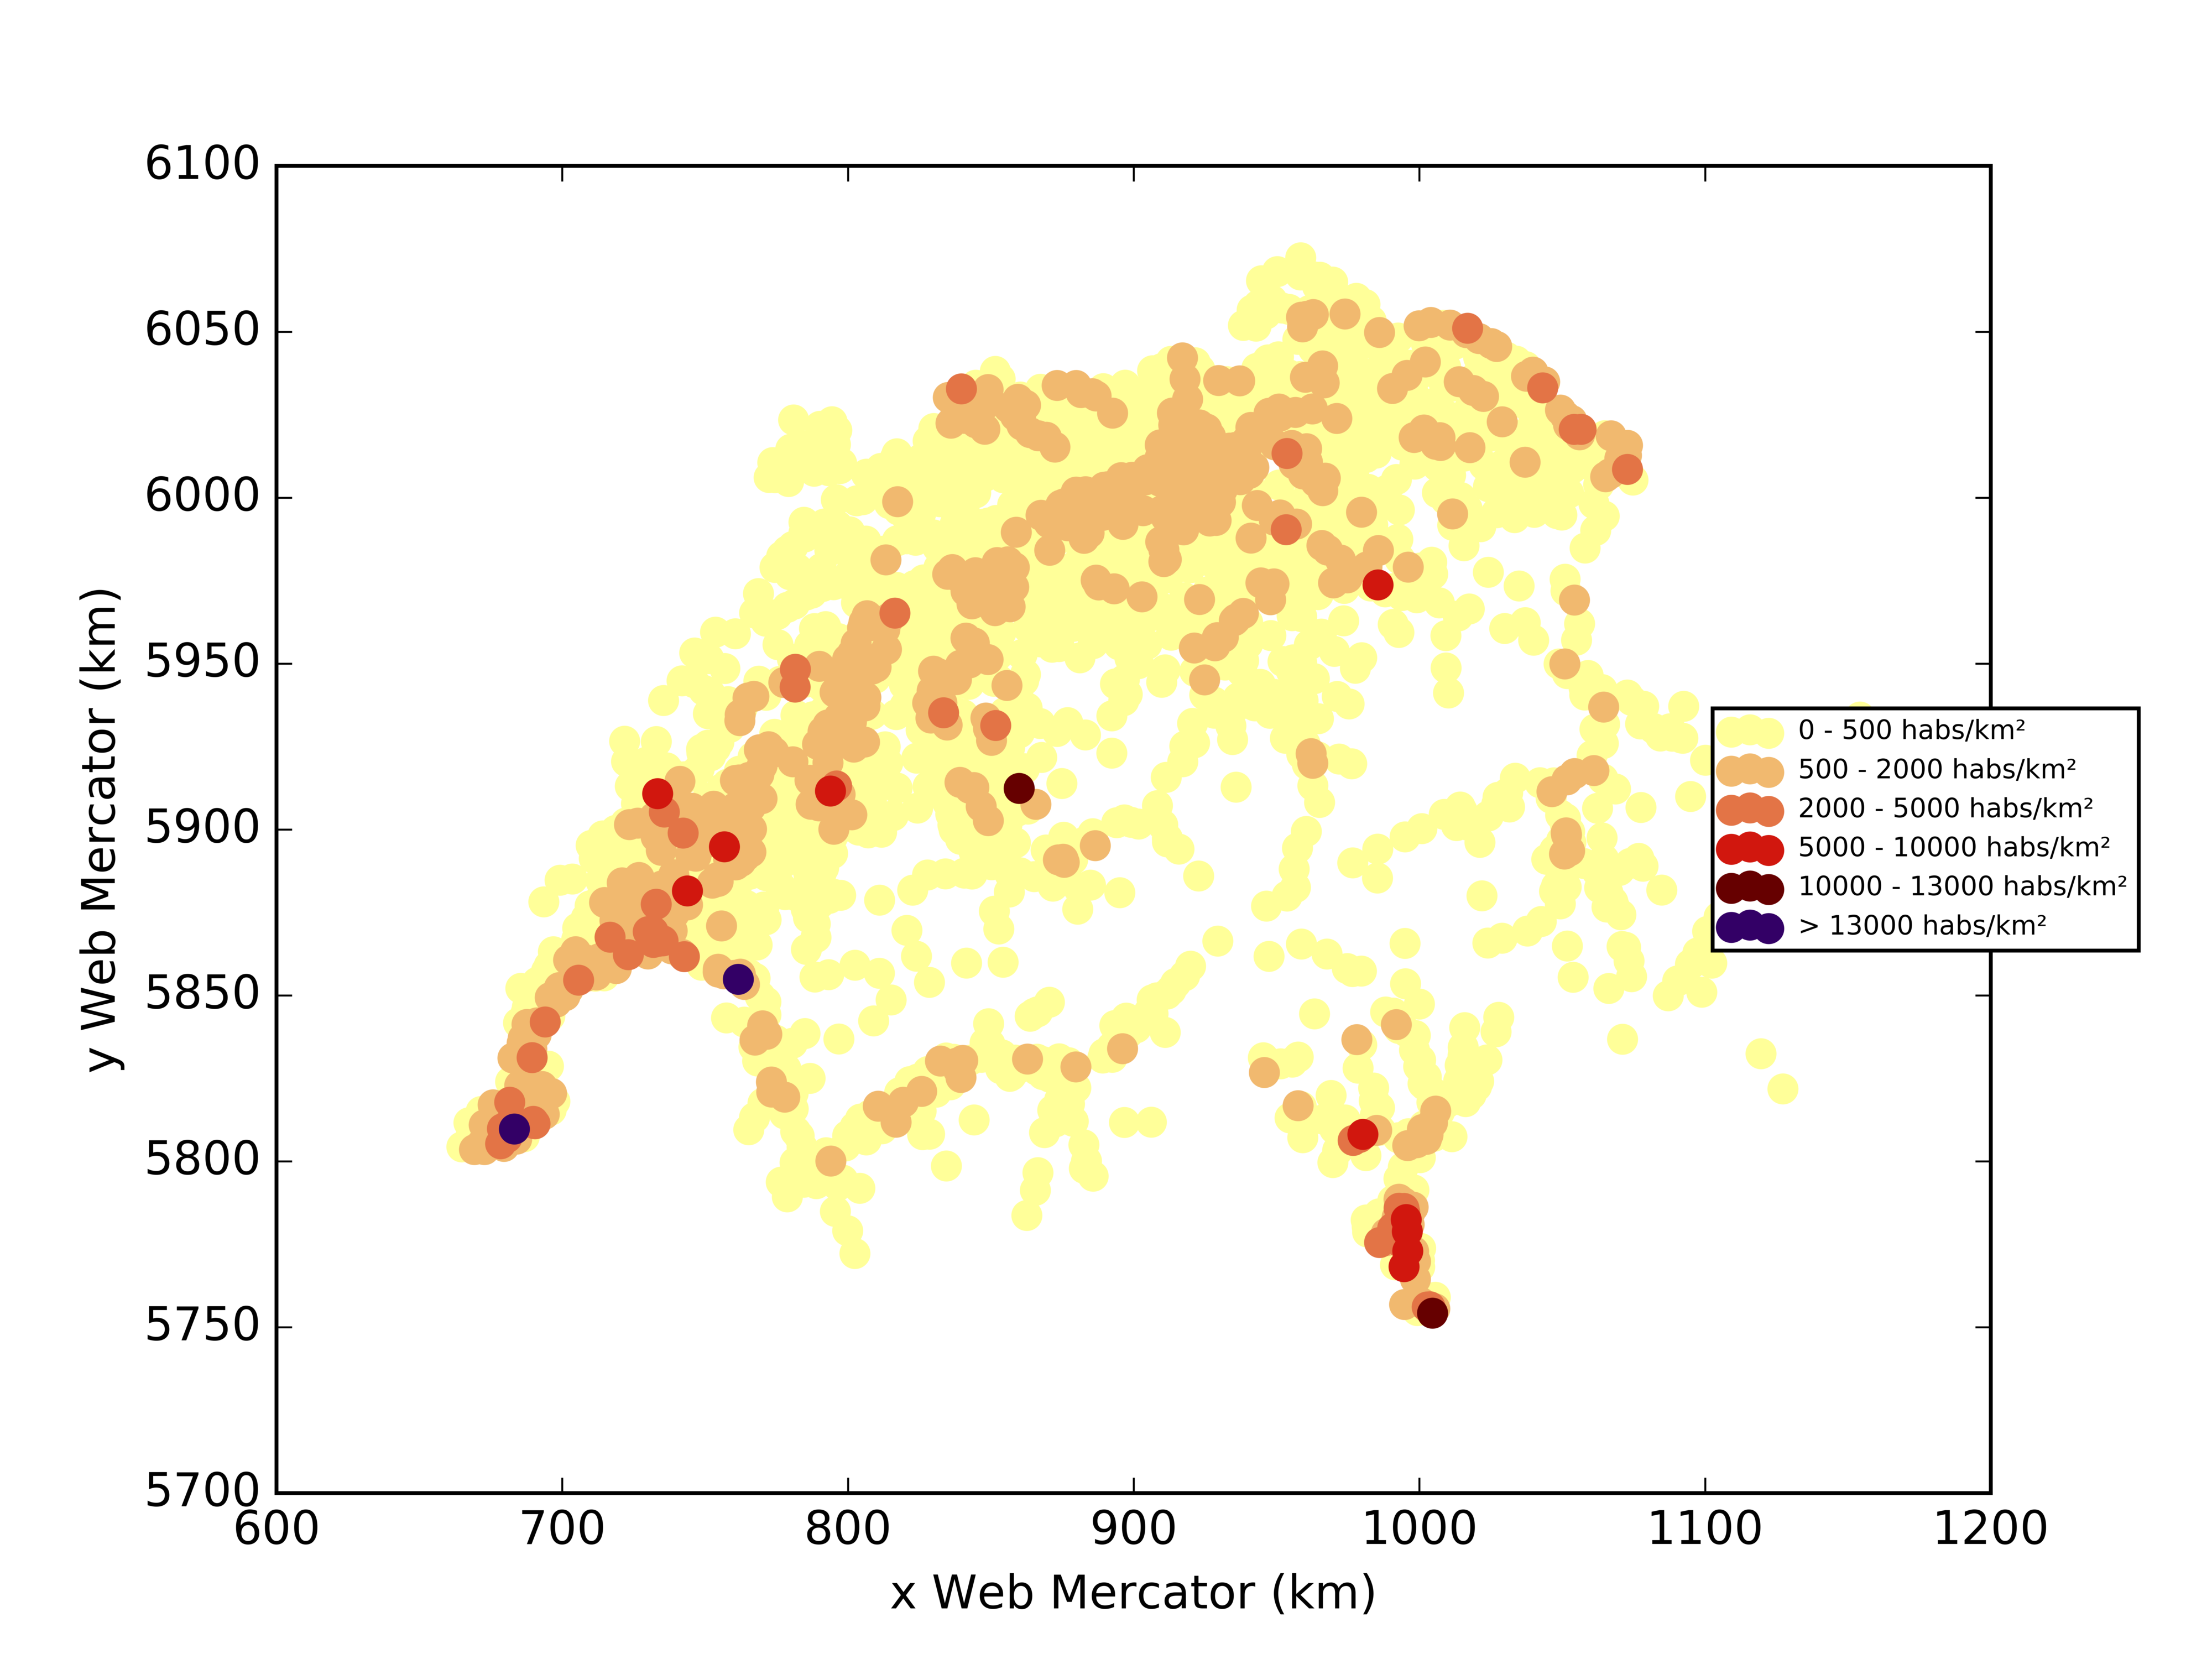
\includegraphics[scale=0.50]{images/Switzerland/nn/density_classification.png}
  \end{overlayarea}
  \begin{overlayarea}{\linewidth}{0.5cm}
    \centering
    \tiny Switzerland density category - prediction\par
  \end{overlayarea}
 \end{column}
\end{columns}
\begin{columns}
 \begin{column}{0.5\textwidth}
 \begin{overlayarea}{\linewidth}{2cm}
  \begin{table}
  \begin{center}
  \begin{adjustbox}{max width=0.7\textwidth}
  {\tiny
  \begin{tabular}{|c|c|c|c|c|c|c|}
    \hline
    \multicolumn{7}{|c|}{{\tiny \begin{bf}Confusion matrix\end{bf}}} \\
    \hline
     & \textbf{1} & \textbf{2} & \textbf{3} & \textbf{4} & \textbf{5} & \textbf{6}\\
    \hline
    \textbf{1} & 32533 & 0 & 0 & 0 & 0 & 0\\
    \hline
    \textbf{2} & 0 & 1252 & 0 & 0 & 0 & 0\\
    \hline
    \textbf{3} & 0 & 0 & 288 & 0 & 0 & 0\\
    \hline
    \textbf{4} & 0 & 0 & 0 & 78 & 0 & 0\\
    \hline
    \textbf{5} & 0 & 0 & 0 & 0 & 15 & 0\\
    \hline
    \textbf{6} & 0 & 0 & 0 & 0 & 0 & 24\\
    \hline
  \end{tabular}
  }
  \end{adjustbox}
  \end{center}
  \end{table}
 \end{overlayarea}
 \end{column}
 \begin{column}{0.5\textwidth}
 \begin{overlayarea}{\linewidth}{2cm}
  \begin{table}
    \begin{center}
    \begin{adjustbox}{max width=0.4\textwidth}
    {\tiny 
    \begin{tabular}{|c|c|}
      \hline
      \multicolumn{2}{|c|}{\begin{bf}Mean score per class\end{bf}} \\
      \hline
      \textbf{category} & \textbf{mean score}\\
      \hline
      \textbf{1} & 100\% \\
      \hline
      \textbf{2} & 100\% \\
      \hline
      \textbf{3} & 100\% \\
      \hline
      \textbf{4} & 100\% \\
      \hline
      \textbf{5} & 100\% \\
      \hline
      \textbf{6} & 100\% \\
      \hline
      \textbf{mean} & 100\% \\
      \hline
    \end{tabular}
    }
    \end{adjustbox}
    \end{center}
  \end{table}
  \end{overlayarea}
\end{column}
\end{columns}
\end{frame}

\begin{frame}
\begin{columns}
 \begin{column}{0.5\textwidth}
  \begin{overlayarea}{\linewidth}{4cm}
    \centering\vfill
    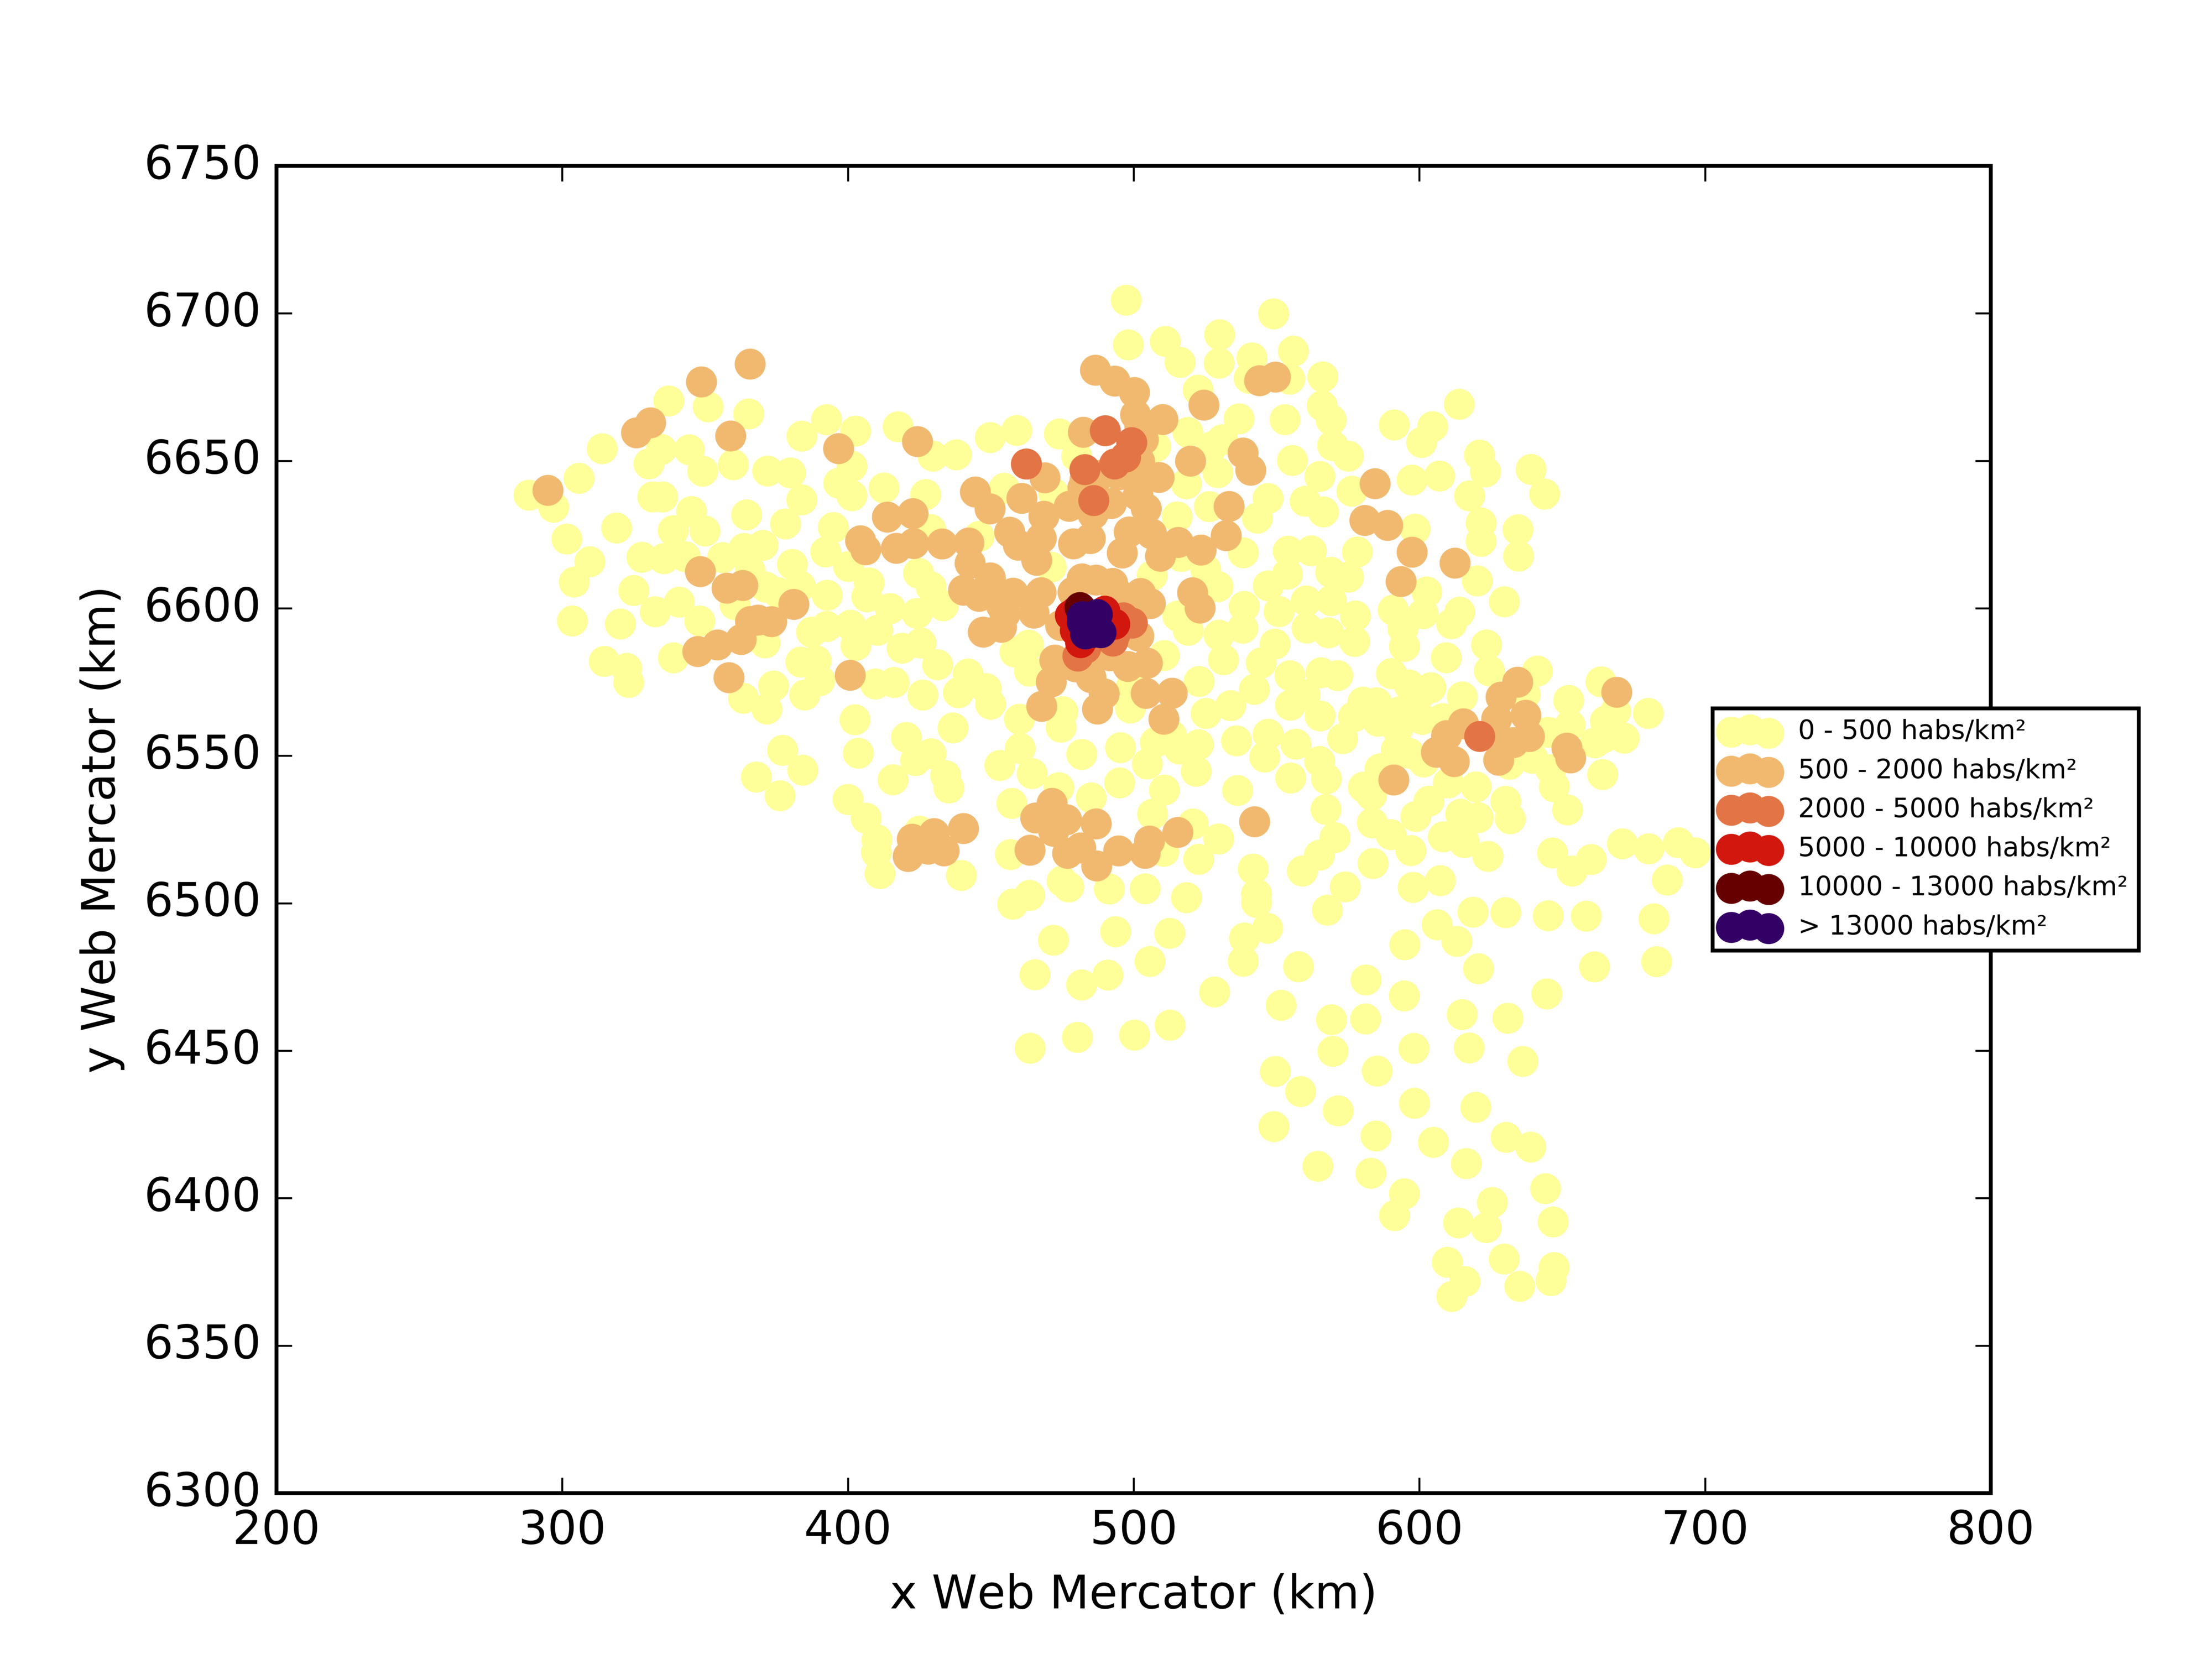
\includegraphics[scale=0.50]{images/Belgium/density_ground_truth.png}
  \end{overlayarea}
  \begin{overlayarea}{\linewidth}{0.5cm}
    \centering
    \tiny Switzerland density category - ground truth\par
  \end{overlayarea}
 \end{column}
 \begin{column}{0.5\textwidth}
  \begin{overlayarea}{\linewidth}{4cm}
    \centering\vfill
    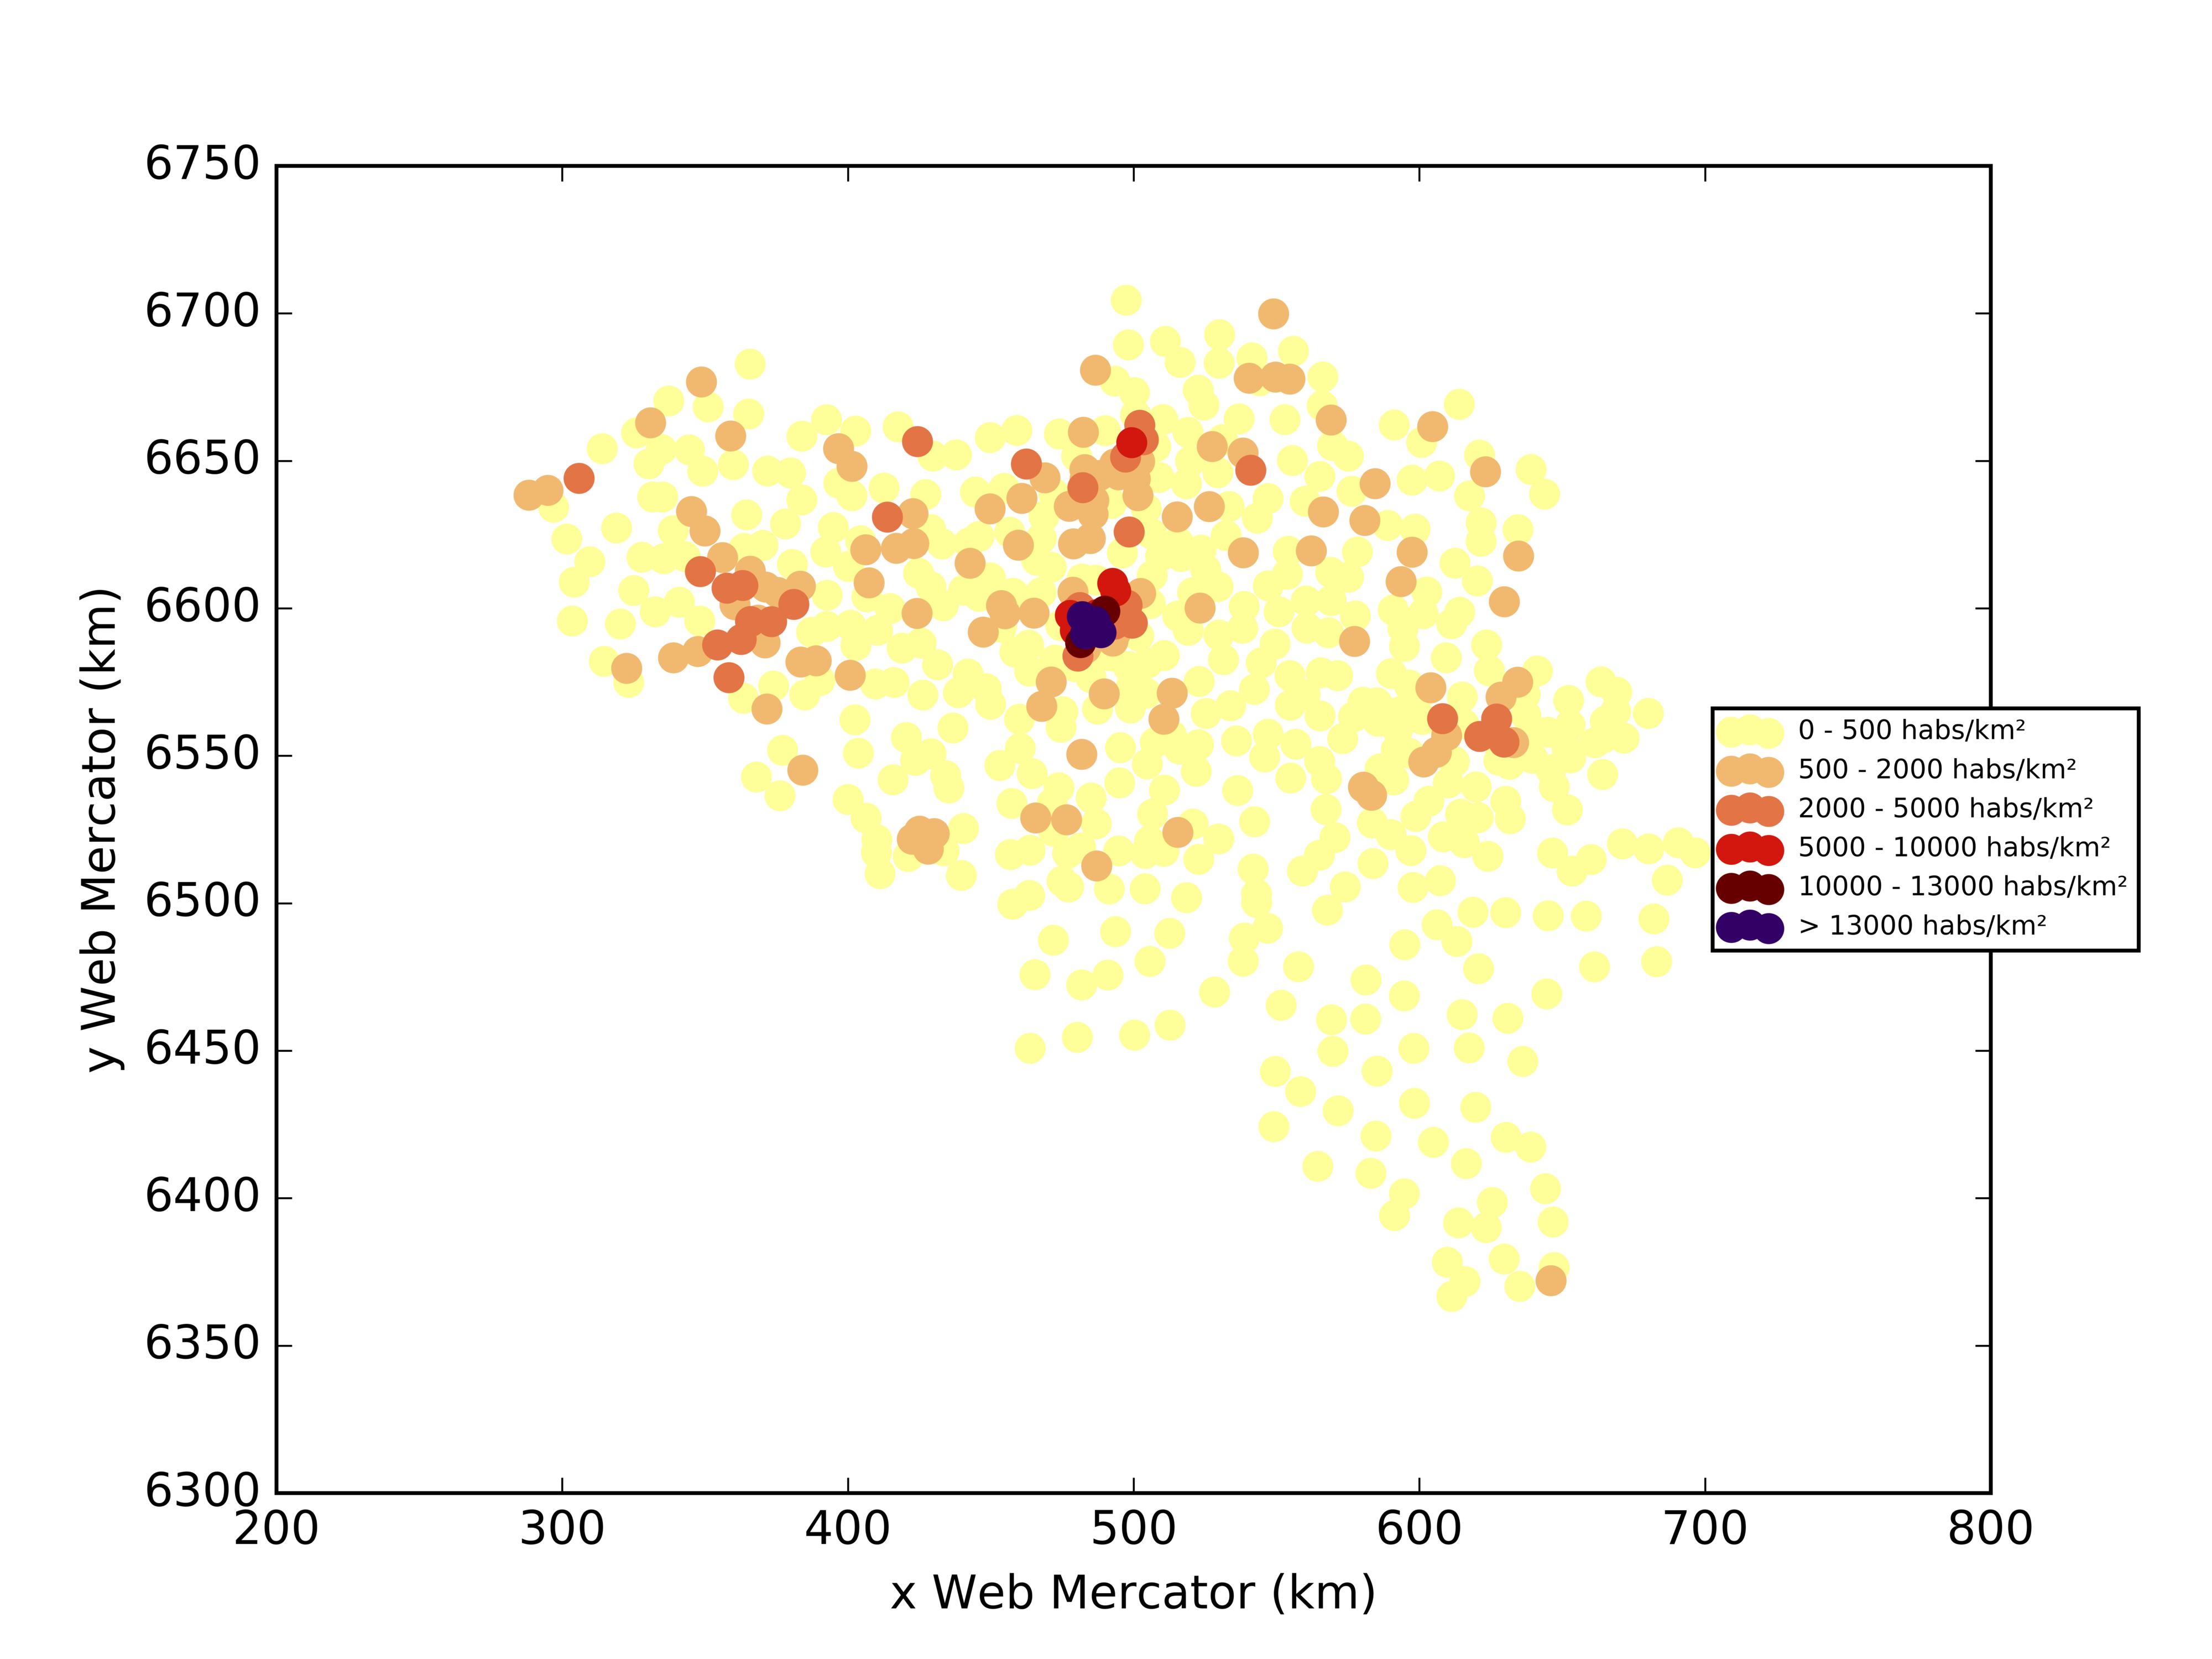
\includegraphics[scale=0.50]{images/Belgium/nn/density_classification.png}
  \end{overlayarea}
  \begin{overlayarea}{\linewidth}{0.5cm}
    \centering
    \tiny Switzerland density category - prediction\par
  \end{overlayarea}
 \end{column}
\end{columns}
\begin{columns}
 \begin{column}{0.5\textwidth}
 \begin{overlayarea}{\linewidth}{2cm}
  \begin{table}
  \begin{center}
  \begin{adjustbox}{max width=0.7\textwidth}
  {\tiny
  \begin{tabular}{|c|c|c|c|c|c|c|}
    \hline
    \multicolumn{7}{|c|}{{\tiny \begin{bf}Confusion matrix\end{bf}}} \\
    \hline
     & \textbf{1} & \textbf{2} & \textbf{3} & \textbf{4} & \textbf{5} & \textbf{6}\\
    \hline
    \textbf{1} & 32533 & 0 & 0 & 0 & 0 & 0\\
    \hline
    \textbf{2} & 0 & 1252 & 0 & 0 & 0 & 0\\
    \hline
    \textbf{3} & 0 & 0 & 288 & 0 & 0 & 0\\
    \hline
    \textbf{4} & 0 & 0 & 0 & 78 & 0 & 0\\
    \hline
    \textbf{5} & 0 & 0 & 0 & 0 & 15 & 0\\
    \hline
    \textbf{6} & 0 & 0 & 0 & 0 & 0 & 24\\
    \hline
  \end{tabular}
  }
  \end{adjustbox}
  \end{center}
  \end{table}
 \end{overlayarea}
 \end{column}
 \begin{column}{0.5\textwidth}
 \begin{overlayarea}{\linewidth}{2cm}
  \begin{table}
    \begin{center}
    \begin{adjustbox}{max width=0.4\textwidth}
    {\tiny 
    \begin{tabular}{|c|c|}
      \hline
      \multicolumn{2}{|c|}{\begin{bf}Mean score per class\end{bf}} \\
      \hline
      \textbf{category} & \textbf{mean score}\\
      \hline
      \textbf{1} & 100\% \\
      \hline
      \textbf{2} & 100\% \\
      \hline
      \textbf{3} & 100\% \\
      \hline
      \textbf{4} & 100\% \\
      \hline
      \textbf{5} & 100\% \\
      \hline
      \textbf{6} & 100\% \\
      \hline
      \textbf{mean} & 100\% \\
      \hline
    \end{tabular}
    }
    \end{adjustbox}
    \end{center}
  \end{table}
  \end{overlayarea}
\end{column}
\end{columns}
\end{frame}

\begin{frame}
\begin{columns}
 \begin{column}{0.5\textwidth}
  \begin{overlayarea}{\linewidth}{4cm}
    \centering\vfill
    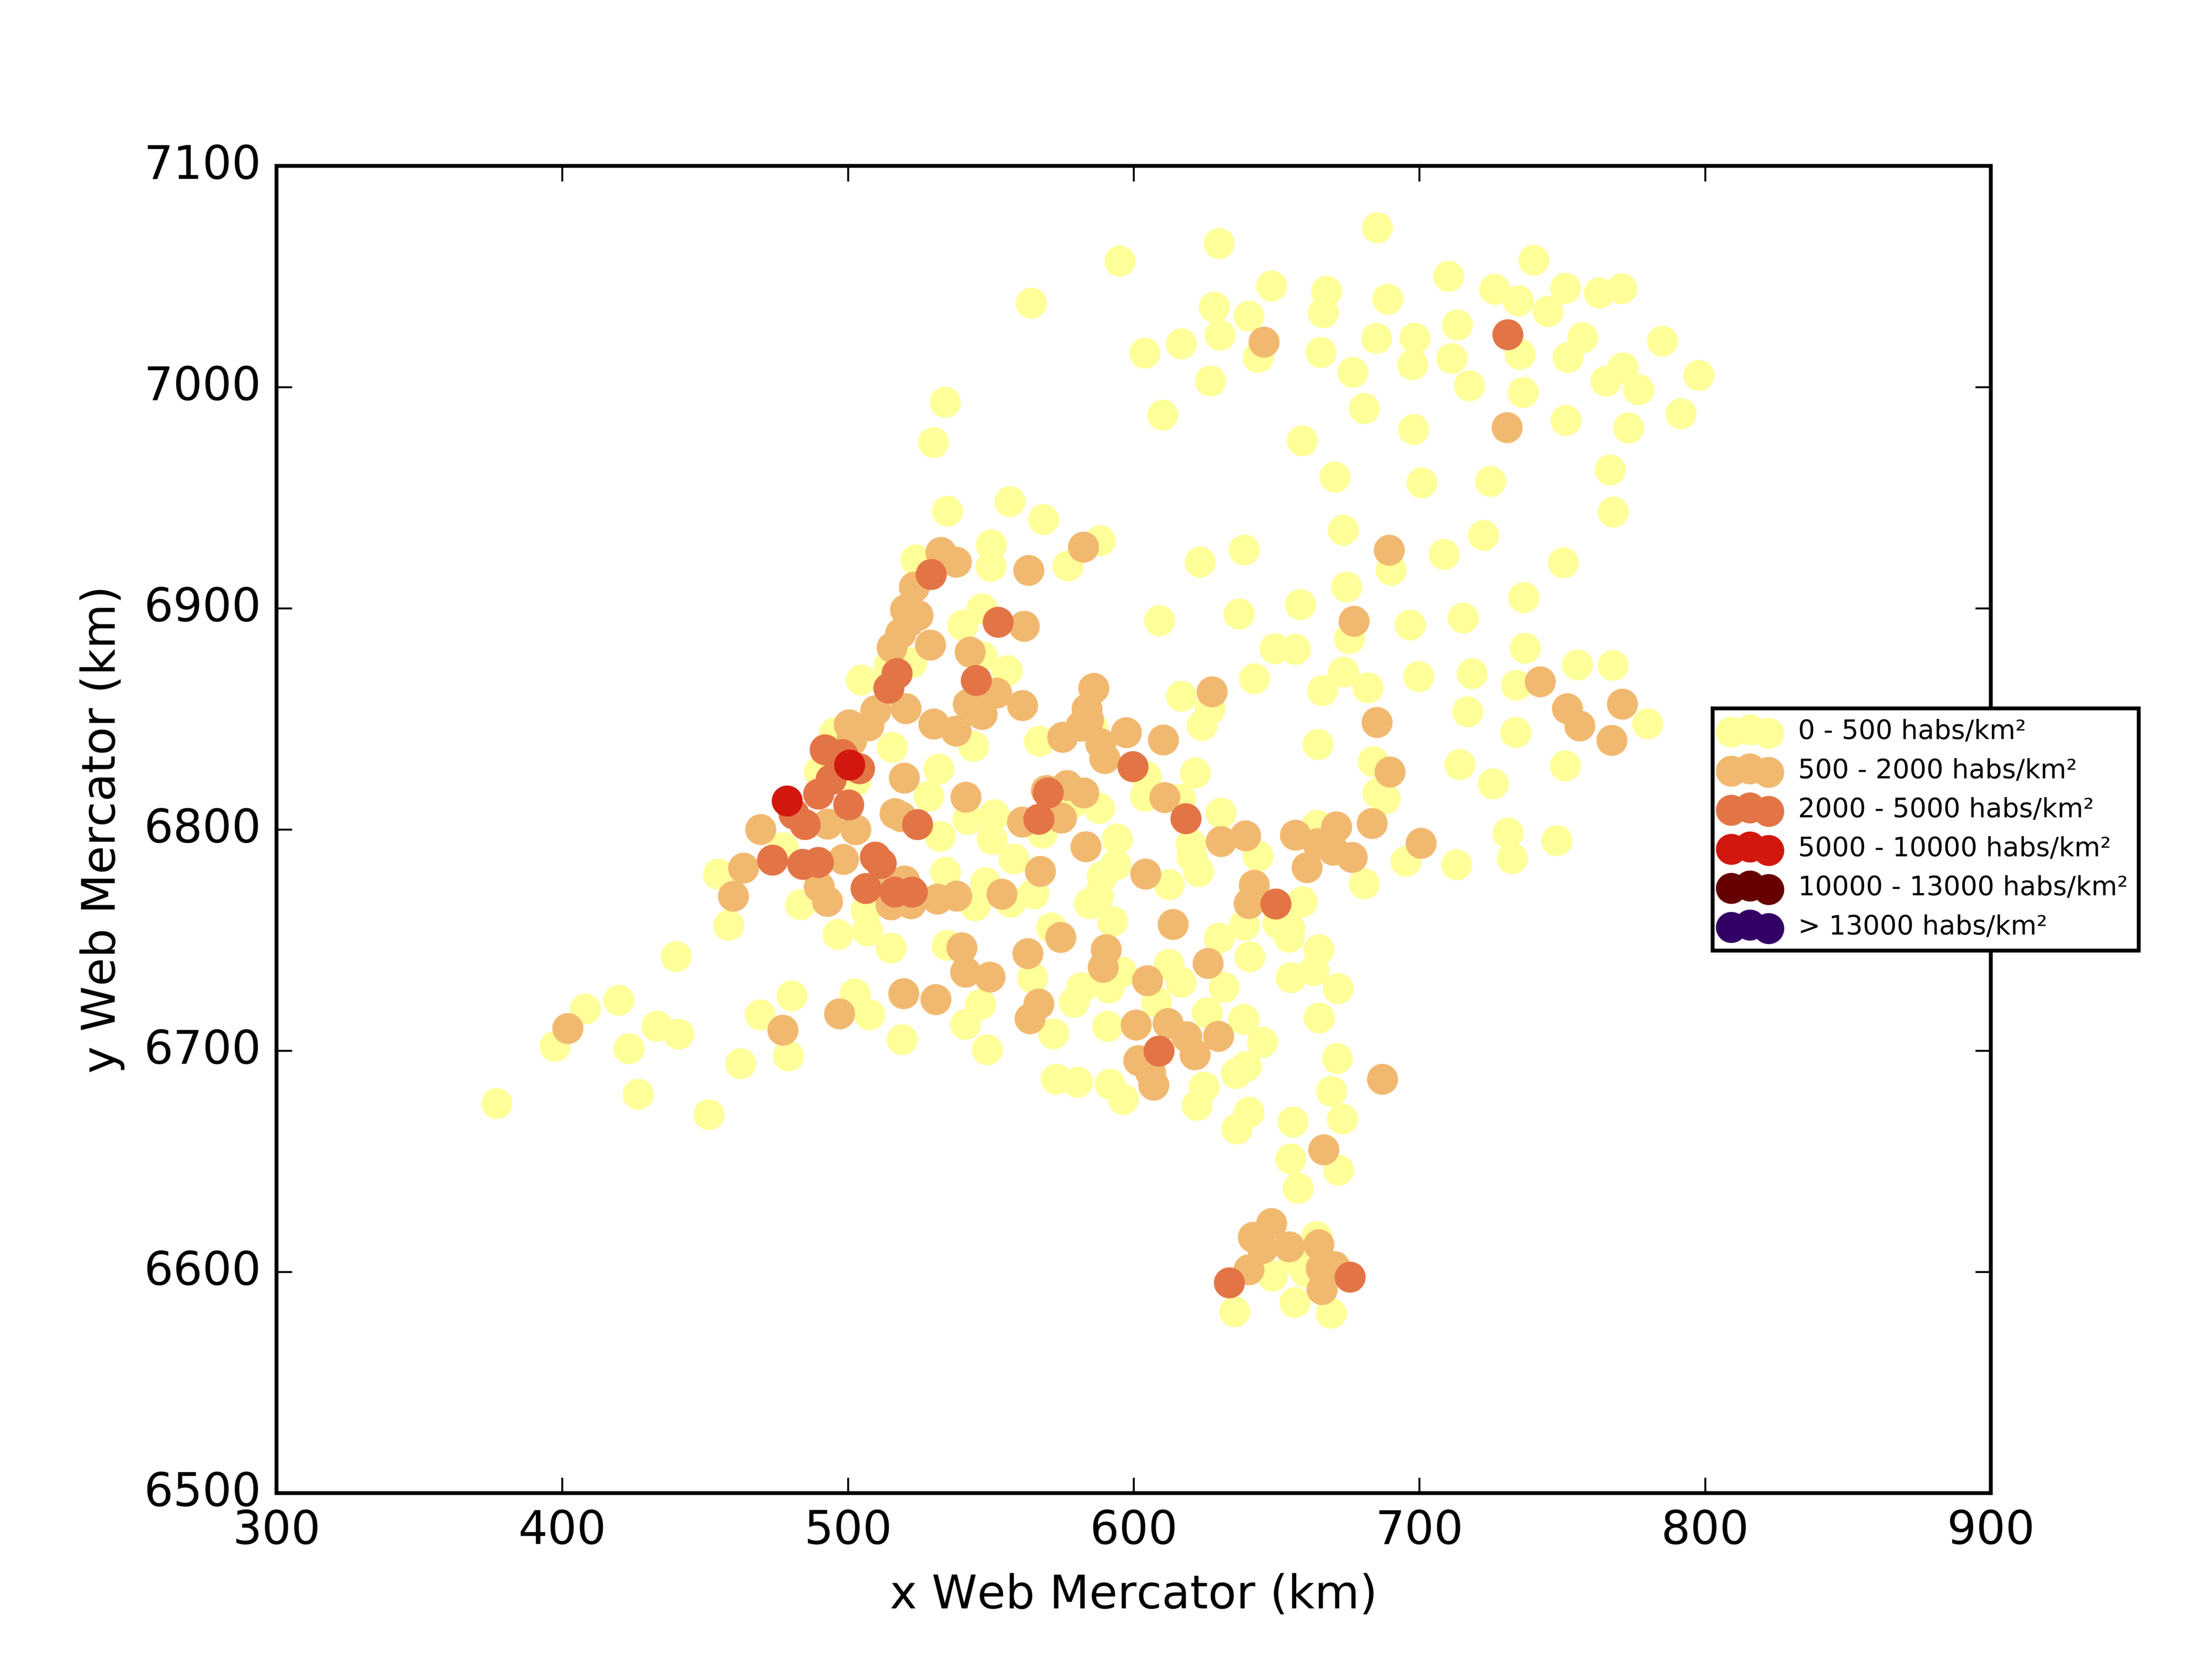
\includegraphics[scale=0.50]{images/Netherlands/density_ground_truth.png}
  \end{overlayarea}
  \begin{overlayarea}{\linewidth}{0.5cm}
    \centering
    \tiny Switzerland density category - ground truth\par
  \end{overlayarea}
 \end{column}
 \begin{column}{0.5\textwidth}
  \begin{overlayarea}{\linewidth}{4cm}
    \centering\vfill
    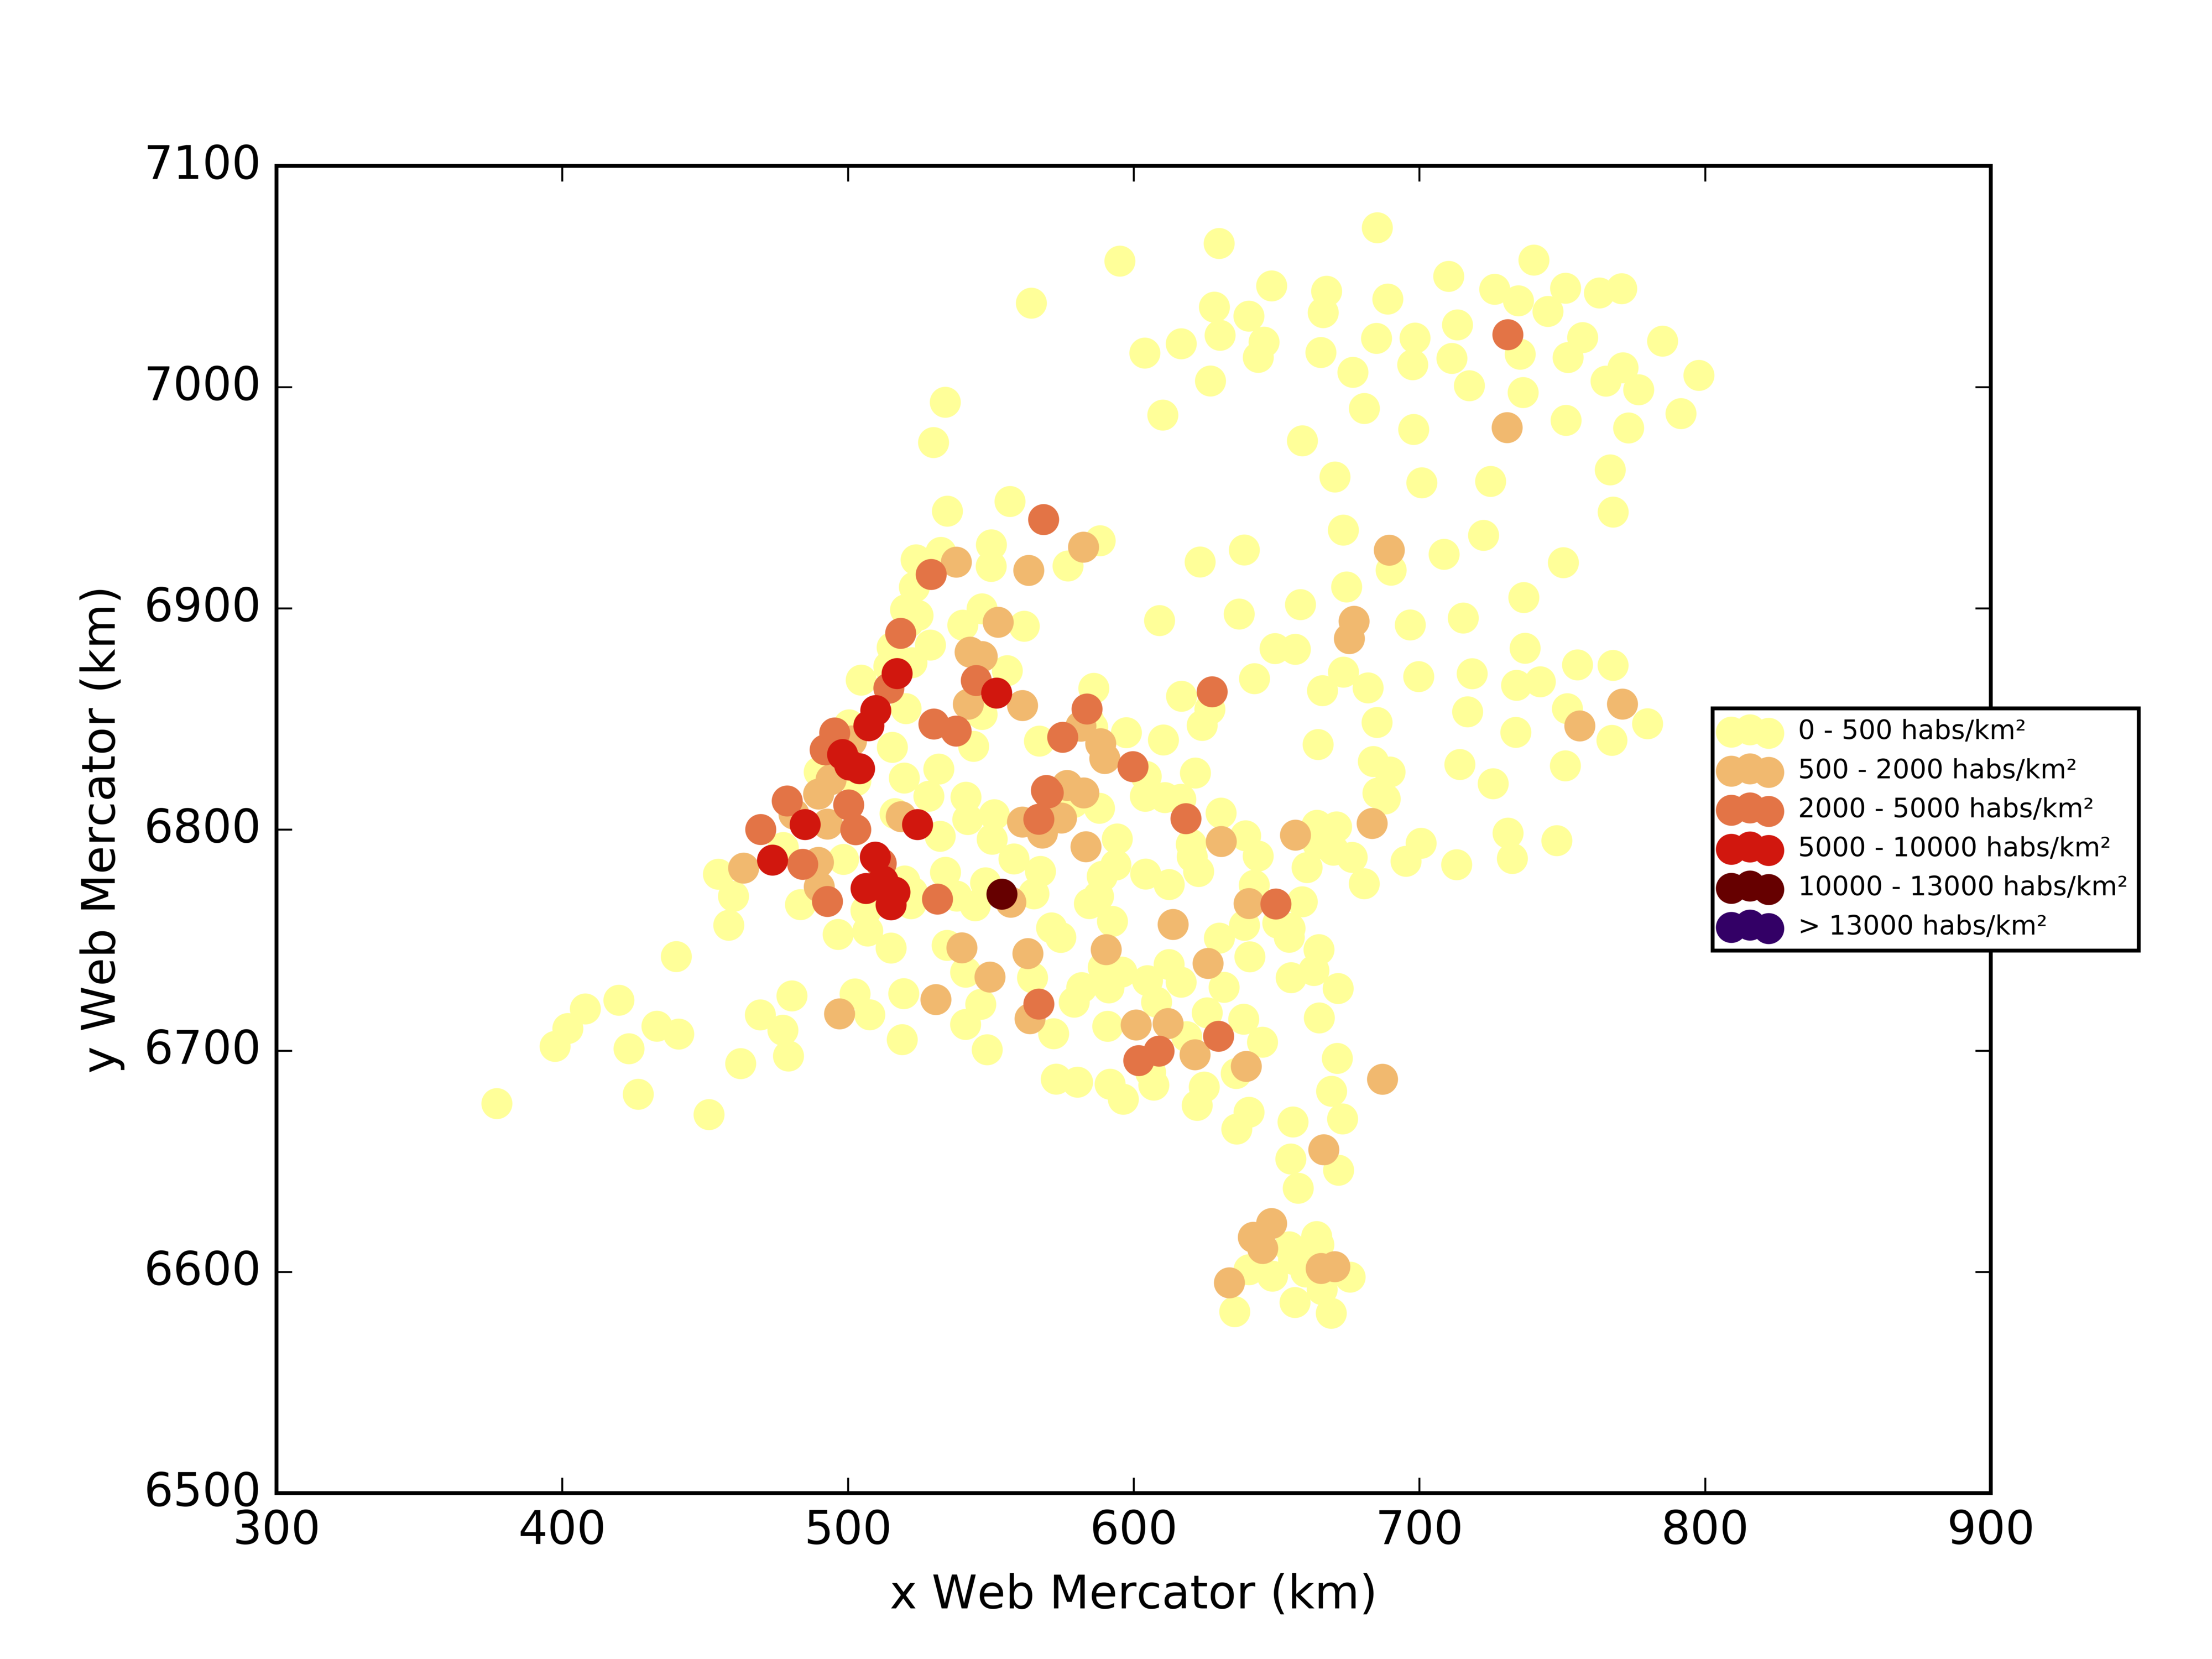
\includegraphics[scale=0.50]{images/Netherlands/nn/density_classification.png}
  \end{overlayarea}
  \begin{overlayarea}{\linewidth}{0.5cm}
    \centering
    \tiny Switzerland density category - prediction\par
  \end{overlayarea}
 \end{column}
\end{columns}
\begin{columns}
 \begin{column}{0.5\textwidth}
 \begin{overlayarea}{\linewidth}{2cm}
  \begin{table}
  \begin{center}
  \begin{adjustbox}{max width=0.7\textwidth}
  {\tiny
  \begin{tabular}{|c|c|c|c|c|c|c|}
    \hline
    \multicolumn{7}{|c|}{{\tiny \begin{bf}Confusion matrix\end{bf}}} \\
    \hline
     & \textbf{1} & \textbf{2} & \textbf{3} & \textbf{4} & \textbf{5} & \textbf{6}\\
    \hline
    \textbf{1} & 32533 & 0 & 0 & 0 & 0 & 0\\
    \hline
    \textbf{2} & 0 & 1252 & 0 & 0 & 0 & 0\\
    \hline
    \textbf{3} & 0 & 0 & 288 & 0 & 0 & 0\\
    \hline
    \textbf{4} & 0 & 0 & 0 & 78 & 0 & 0\\
    \hline
    \textbf{5} & 0 & 0 & 0 & 0 & 15 & 0\\
    \hline
    \textbf{6} & 0 & 0 & 0 & 0 & 0 & 24\\
    \hline
  \end{tabular}
  }
  \end{adjustbox}
  \end{center}
  \end{table}
 \end{overlayarea}
 \end{column}
 \begin{column}{0.5\textwidth}
 \begin{overlayarea}{\linewidth}{2cm}
  \begin{table}
    \begin{center}
    \begin{adjustbox}{max width=0.4\textwidth}
    {\tiny 
    \begin{tabular}{|c|c|}
      \hline
      \multicolumn{2}{|c|}{\begin{bf}Mean score per class\end{bf}} \\
      \hline
      \textbf{category} & \textbf{mean score}\\
      \hline
      \textbf{1} & 100\% \\
      \hline
      \textbf{2} & 100\% \\
      \hline
      \textbf{3} & 100\% \\
      \hline
      \textbf{4} & 100\% \\
      \hline
      \textbf{5} & 100\% \\
      \hline
      \textbf{6} & 100\% \\
      \hline
      \textbf{mean} & 100\% \\
      \hline
    \end{tabular}
    }
    \end{adjustbox}
    \end{center}
  \end{table}
  \end{overlayarea}
\end{column}
\end{columns}
\end{frame}

\subsection{Support-Vector Machine (Gaussian Kernel)}

\subsection{Convolutional Neura Networks}
\end{document}
